\chapter{Pixels Detectors for the new ATLAS Inner Tracker}
\label{chap:ITk}

In this Chapter the Pixel Detector of the new ATLAS Inner Tracker (ITk) of the ATLAS detector will be discussed. It is intended to be ready 
for  the data taking in 2026, in time for the beginning of the High Luminosity phase of the LHC (HL-LHC). 
The plans for the upgrades of the LHC are presented in Section~\ref{sec:HL-LHC}, along with the 
physics case and the list of ATLAS sub detector upgrades for the Phase-II; 
Section~\ref{sec:NewTracker} will cover the performance and specifications for the new ATLAS ITk. 
After describing the R\&D efforts for ITk pixels detectors in general (Section~\ref{sec:ITkPixels}), 
in Section~\ref{sec:radhardpixels} results for radiation hard pixel sensors will be presented. 
The concept of slim edge, already applied to IBL pixel sensors (Section~\ref{sec:IBLoverview}) will be 
pushed to its limits for the ITk pixels sensors; this topic will be discussed in details in 
Section~\ref{sec:edgeless}, together with results from beam tests. 
Finally conclusions and perspectives will be drawn in Section~\ref{sec:itksummary}.



\section{High Luminosity LHC and the Phase-II of the LHC experiments}
\label{sec:HL-LHC}

The timeline of the CERN LHC is presented in Figure~\ref{fig:HL-LHC-plan-2016-01}, together 
with the future plans. The High Luminosity LHC (HL-LHC)~\cite{HL_LHC} is a project, recently 
approved~\cite{HL-LHCApproval},  to upgrade the existing LHC to a high luminosity machine, 
capable to deliver an instantaneous luminosity of $L=7.5\times10^{34}$/cm$^{2}$/s; as a 
reminder the design luminosity of LHC is of $L=1.0\times10^{34}$/cm$^{2}$/s.
\begin{figure}[!htpb]
\centering
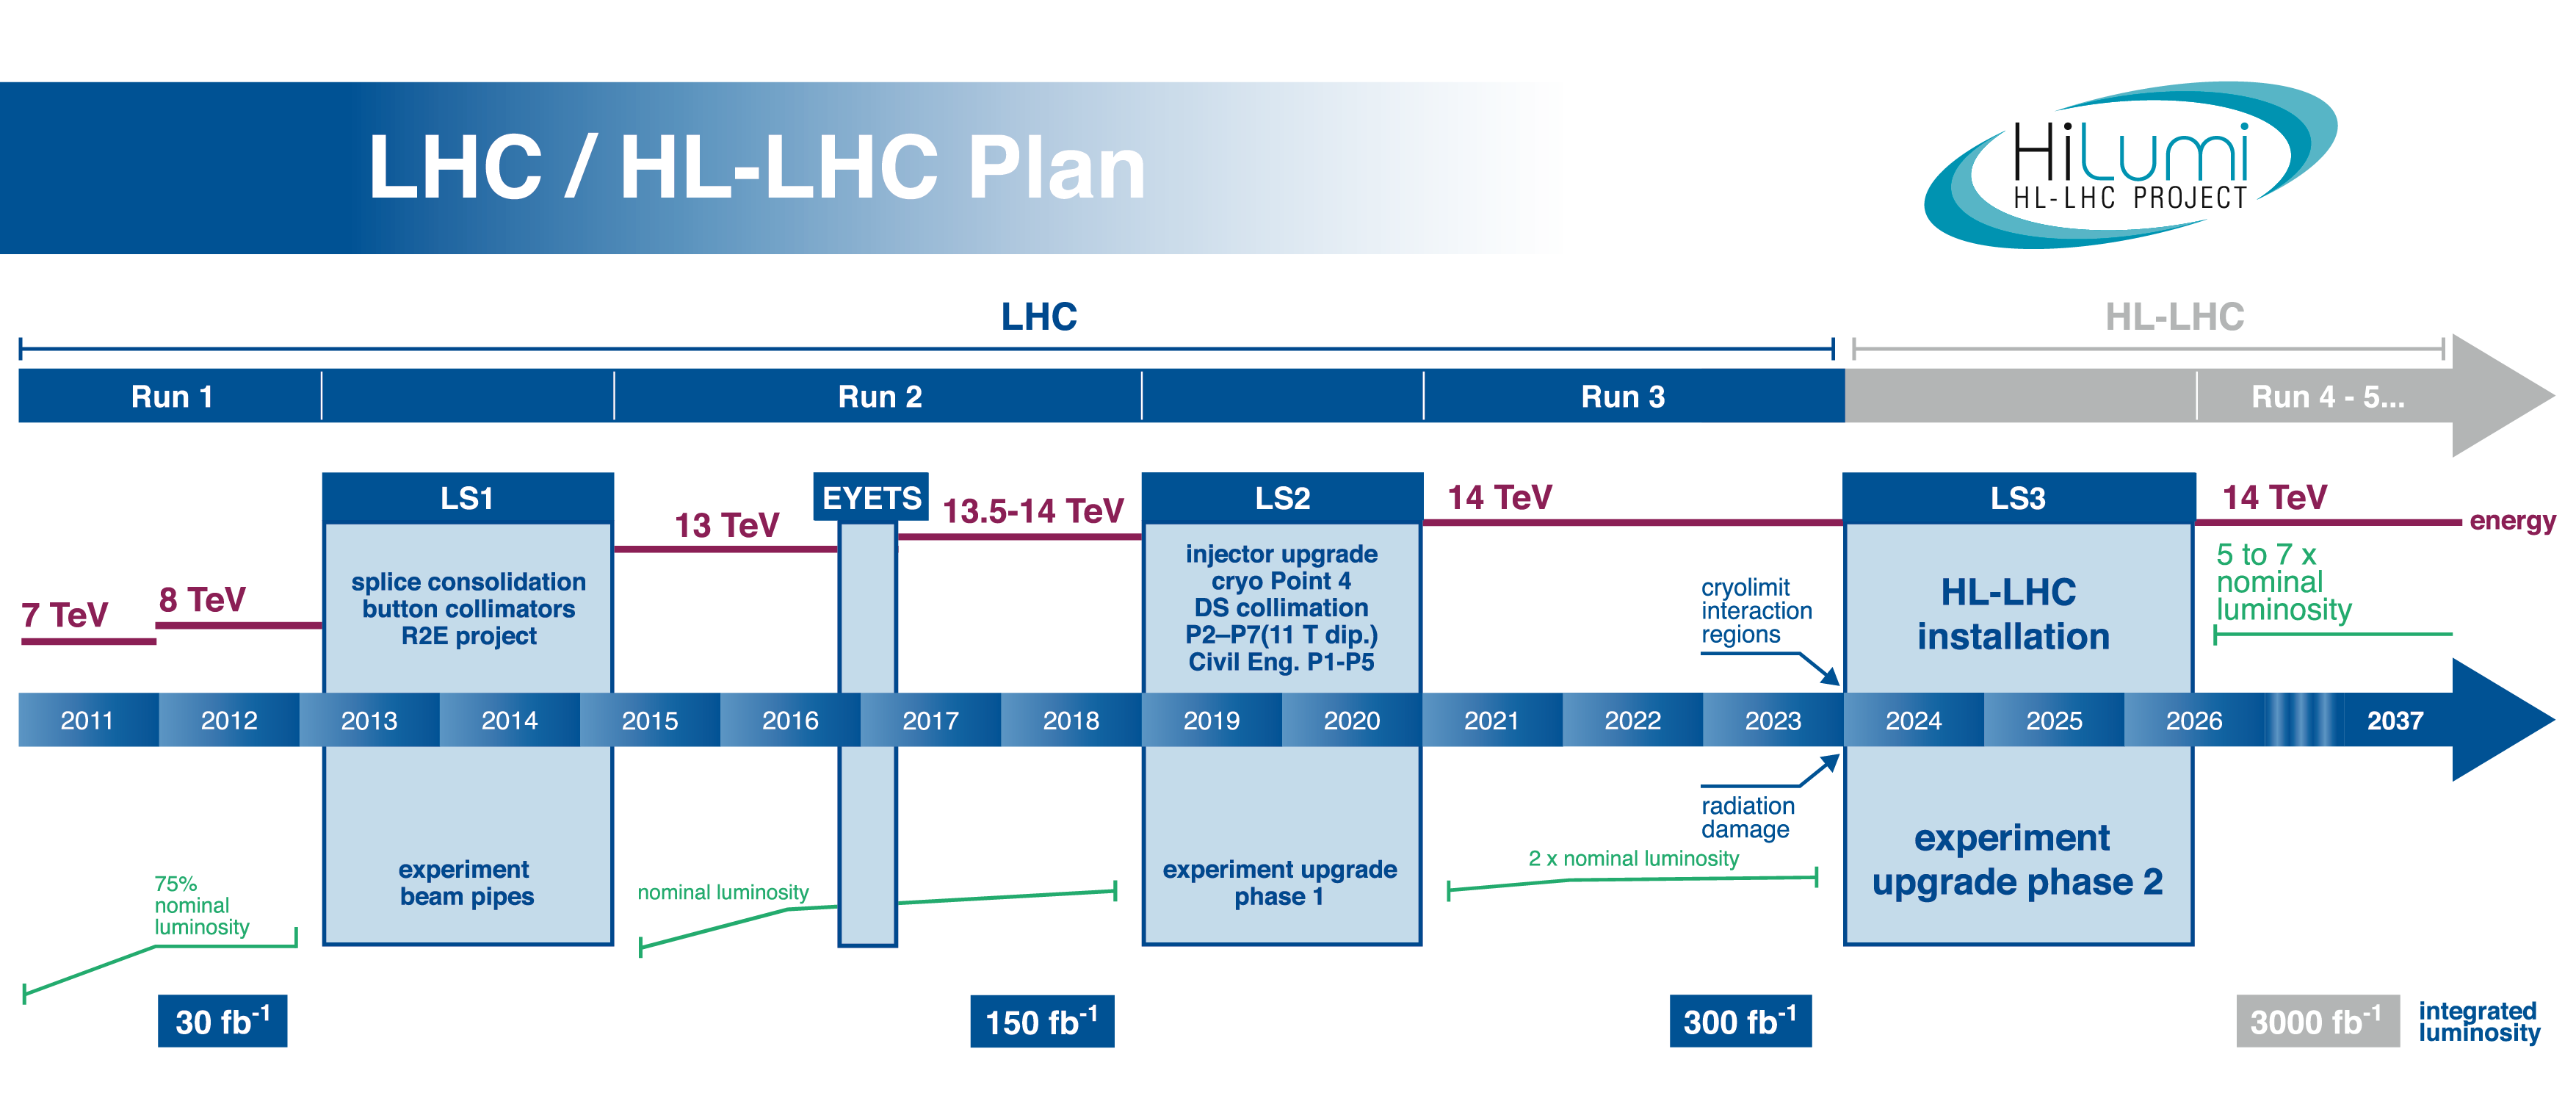
\includegraphics[width=1.0\textwidth]{HL-LHC-plan-2016-01.png}
\caption{\label{fig:HL-LHC-plan-2016-01}LHC/ HL-LHC Plan (last update 22.02.2016, after~\cite{HL_LHC})}
\end{figure}
After the HL-LHC upgrade completion the data taking  is expected to restart in 2026; the goal 
is to integrate a dataset of 3000~\invfb by 2037; there is an option to extend this program to arrive 
at 4000~\invfb.

As it can be seen in Figure~\ref{fig:HL-LHC-plan-2016-01} the upgrade plans don't include any increase 
of the center-of-mass energy $\sqrt{s}$: the main motivation for the HL-LHC project is 
reducing the error halving time. Indeed, taking data beyond 2023 at the same instantaneous luminosity of 
Run~3 would imply  to take data for more than 15 years to reduce the statistical error by a factor of 2.

The large dataset at the end of the so-called Phase 2 (or {\it} Phase-II) for the experiments should enable 
a  large program of precision measurements of the Higgs boson and New Physics (NP) discoveries. 
As an example of the potential of the HL-LHC dataset, the projected precision on coupling of the Higgs
 boson to muons is of about 7\% with  3000~\invfb; the Higgs 
trilinear self coupling parameter $\lambda_{HHH}$ can be probed at about 1 $\sigma$ significance 
in the range $-0.8<\lambda_{HHH}/\lambda_{SM}<7.7$ ($\lambda_{SM}$ is the SM predicted value) 
in the final state $HH\to\b\bbar\gamma\gamma$~\cite{ATL-PHYS-PUB-2014-016}. 
For what concerns NP potential discoveries, as an example, with the expected HL-LHC dataset the 
supersymmetric top quark partner $\widetilde{t}$ discovery mass range extends up to 480~GeV, and the exclusion one to 700~GeV~\cite{ATL-PHYS-PUB-2016-022};
for the electroweak SUSY particles a factor of ten increase in luminosity translates into a 30-40\% increase in mass reach. Other than SUSY the physics program 
during the Phase-II of the LHC experiments include searches of   vector bosons resonances like 
$W',Z'$, 
extra dimensions and more~\cite{ATLASLoIPhaseII}.

The high luminosity foreseen for the Phase-II implies a much harsher environment than in Run~2 
for the ATLAS sub-detectors; indeed high luminosity means higher event rate, more pileup events 
and higher radiation doses and fluences. 
To cope with the severe data taking conditions expected at the HL-LHC it is planned to 
upgrade the  ATLAS detector~\cite{ATLASLoIPhaseII,ATLASITkScopingDocument}. Upgrades include:

\begin{itemize}
\item a longer latency trigger system, to cope with higher event rates,
\item new inner muon barrel trigger chambers, to assure redundancy and improve efficiency,
\item upgrading the tile calorimeter electronics, since the actual system will not survive the doses expected by the time of HL-LHC and
\item a complete new silicon only tracker, with coverage down to pseudorapidity $|\eta|=4$, the {\it Inner Tracker} (ITk)
\end{itemize} 

The constraints, requirements, layout and expected performance of the proposed ATLAS ITk will 
be discussed in the next Section.

\section{The Quest for a New ATLAS Inner Tracker}
\label{sec:NewTracker}

The new ATLAS  Inner Tracker will have to face unprecedented levels of radiation doses and fluences, 
pileup events and events rate. Table~\ref{tab:ITkConditions} summarises some of the most important figures.

\begin{table}[!htpb]
\centering
\caption{\label{tab:ITkConditions}Environment conditions for the inner detector at the LHC and HL-LHC}
\begin{tabular}{lcc}
\hline
Parameter & LHC & HL-LHC \\
\hline
\hline
instantaneous luminosity $L$	 [cm$^{-2}$s$^{-1}$] & $1.0\times10^{34}$ &  $7.5\times10^{34}$ \\
average number of pileup events $\mu$ & 25 & 200\\
track rate density for the innermost pixel layer $\mathcal{N}$ [MHz~cm$^{-2}$] & 0.25 & 2 \\ 
fluence to the innermost pixel layer $\Phi$ [ 1 MeV $n_\text{eq}/\text{cm}^2$] & 5$\times10^{15}$ & 2$\times10^{16}$ \\
total ionising dose to the innermost pixel layer TID [MRad] & 160  & 1700 \\
\hline
\end{tabular}
\end{table}

Within this hostile environment the ITk will have to guarantee the same level of performance  or better 
of the ATLAS Inner Detector (ID).
The project is presented  in a series of documents, from the ``Letter of Intent for the Phase-II Upgrade of the ATLAS Experiment''~\cite{ATLASLoIPhaseII} to the ``ATLAS Phase-II Upgrade Scoping Document''~\cite{ATLASITkScopingDocument}. Technical Design Report (TDR) for strip detector of the 
ITk was recently published~\cite{ITkStripsTDR}; the ITk pixel detector TDR is due by the end of 2017.
This Section is built on those documents.




\subsection{Performance Requirements of the ITk}
In what follows a short list of performance requirements of the ITk.

\paragraph{Track Reconstruction Efficiency}
The required 
track reconstruction efficiency in the central part ($|\eta|<2.7$) has to be above 99\% for muons with 
$p_T$ above 3~GeV/c, above 85\% for pions (electrons) with 
$p_T$ above 1(5)~GeV/c.  Fake tracks rate has to be kept below 1\% to avoid degrading resolution of 
objects built using tracks, like tracks jets.

\paragraph{Track Resolution and Vertex Reconstrucion}
The resolution on transverse momentum will be better than 0.5\% up $|\eta|=1$ for muons of 100~GeV/c 
$p_T$ and will degrade moderately till $|\eta|=2$. For $|\eta|\ge2.7$ the solenoid field diminishes, 
particularly at low radius, leading to poorer $p_T$ resolution. 
Resolution on longitudinal (transverse) parameter $d_0(z_0)$ are required to be better than 100~$\mu$m 
in the very central region $|\eta|<0.5$ for tracks with $p_T$~=~1GeV/c and better than 8 (50)~$\mu$m  
in the limit of very large transverse momentum.  
 
 With 200 pile-up events, the mean separation of primary vertices is typically less than 1~mm.
 It is therefore not possible for all vertices in a triggered event to be reconstructed individually. However, it is important that high transverse momentum objects (muons, electrons and tracks in high transverse energy jets) coming from a common vertex can all be correctly associated to the same vertex with good efficiency.
  This requirement corresponds, in the case of $\t\tbar$ events, to the probability of the $\t\tbar$  vertex being among the reconstructed vertices having to be greater than 0.95. In addition, the probability that the 
$\t\tbar$  decay is associated to the correct reconstructed vertex should be greater than 0.90.
 
 
 Tracking-reconstruction efficiency and minimisation of multiple scattering effects requirements impose a 
 low material budget. For the ITk, generally it is required to be in total <1 $\X_0$ up to $|\eta|\le2.7$.
 In Figure~\ref{fig:ITk_X0}.
  The ITk material budget is around 30\% lower in the region $|\eta|\le4.0$, compared to the Run~2 detector.
\begin{figure}[!htpb]
\centering
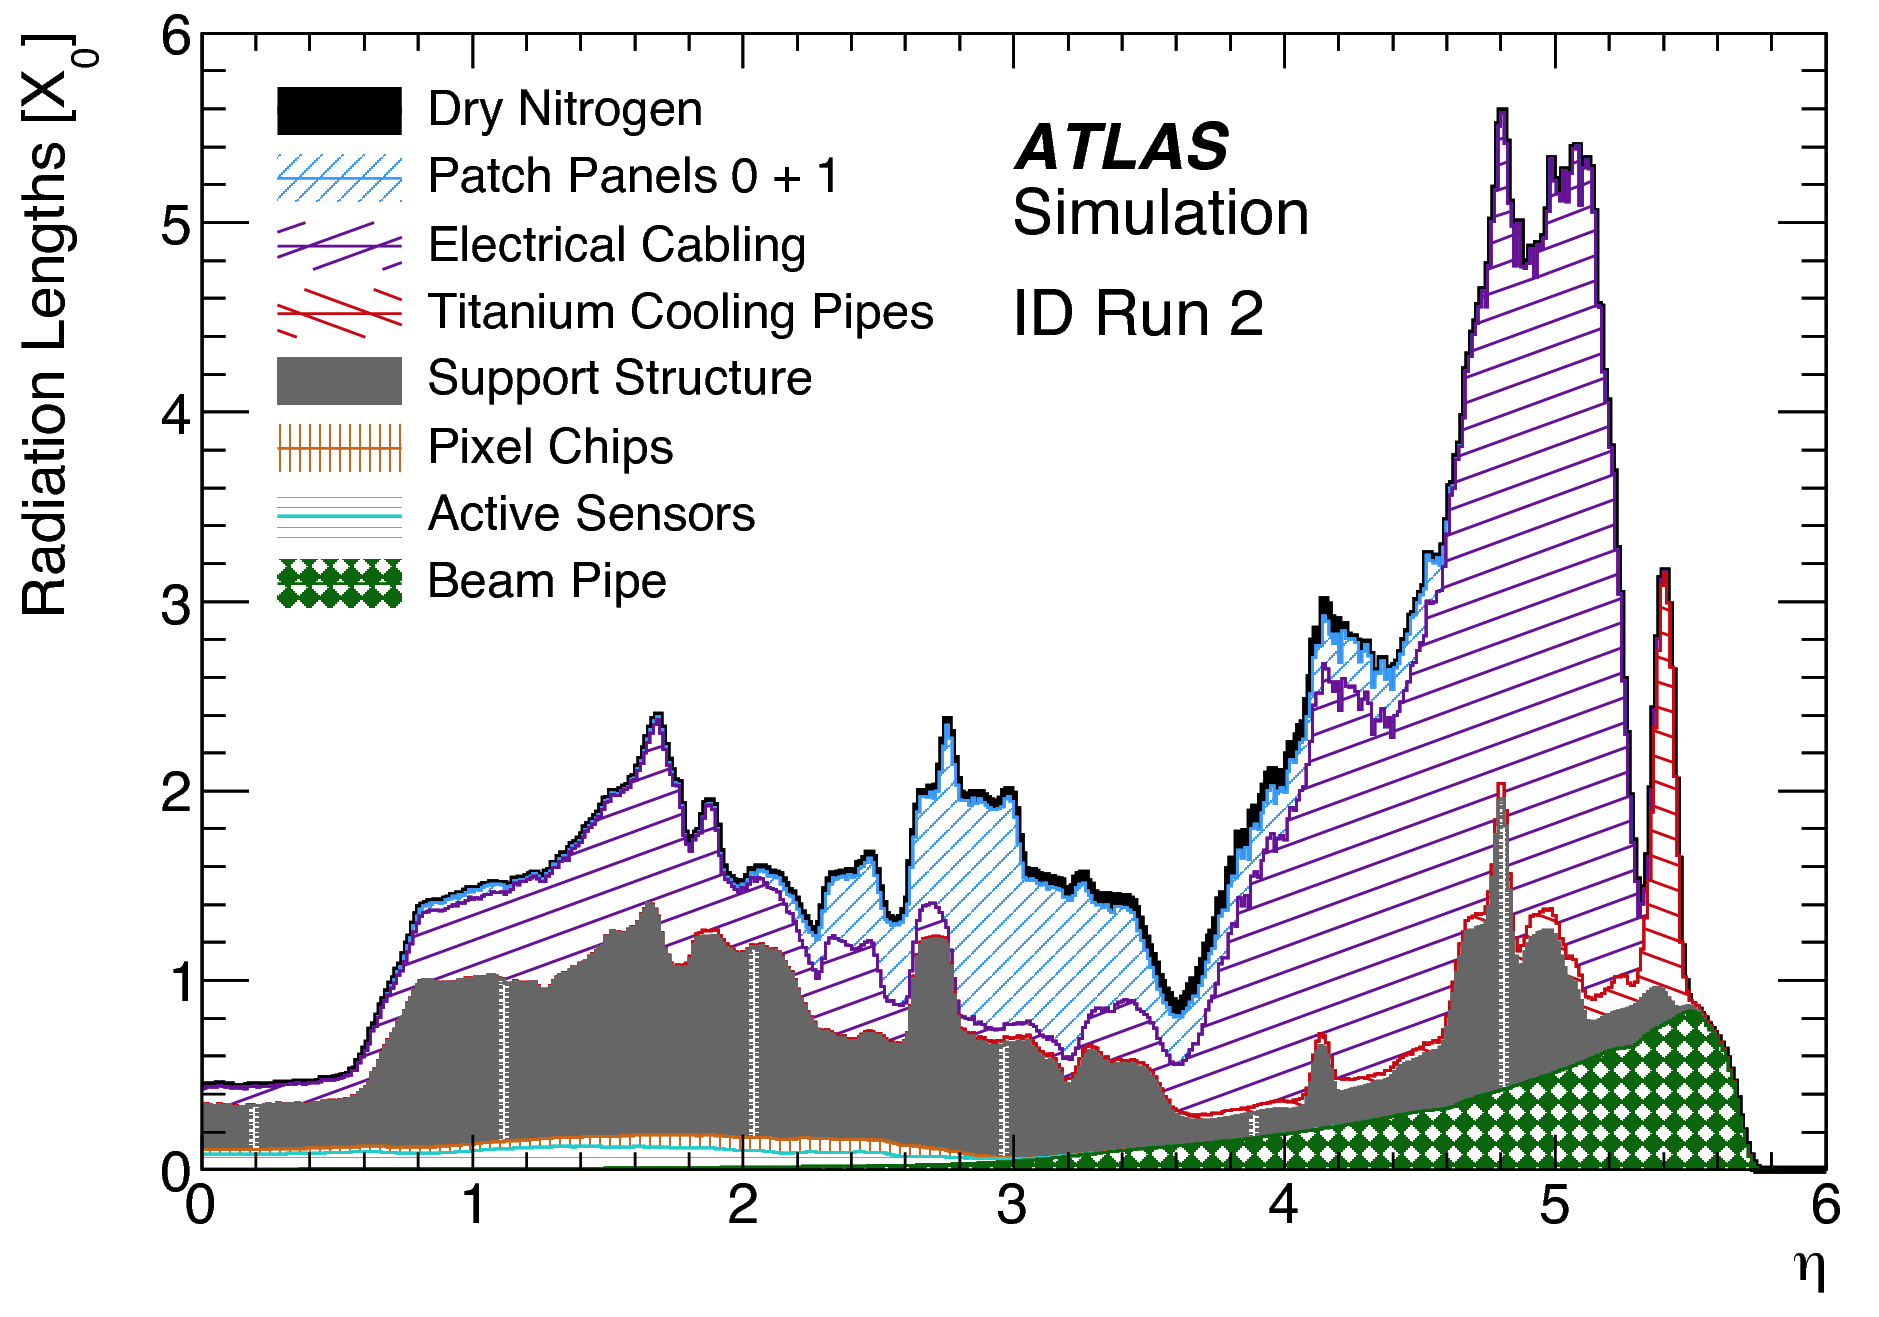
\includegraphics[width=0.49\textwidth]{ID_X0.png}
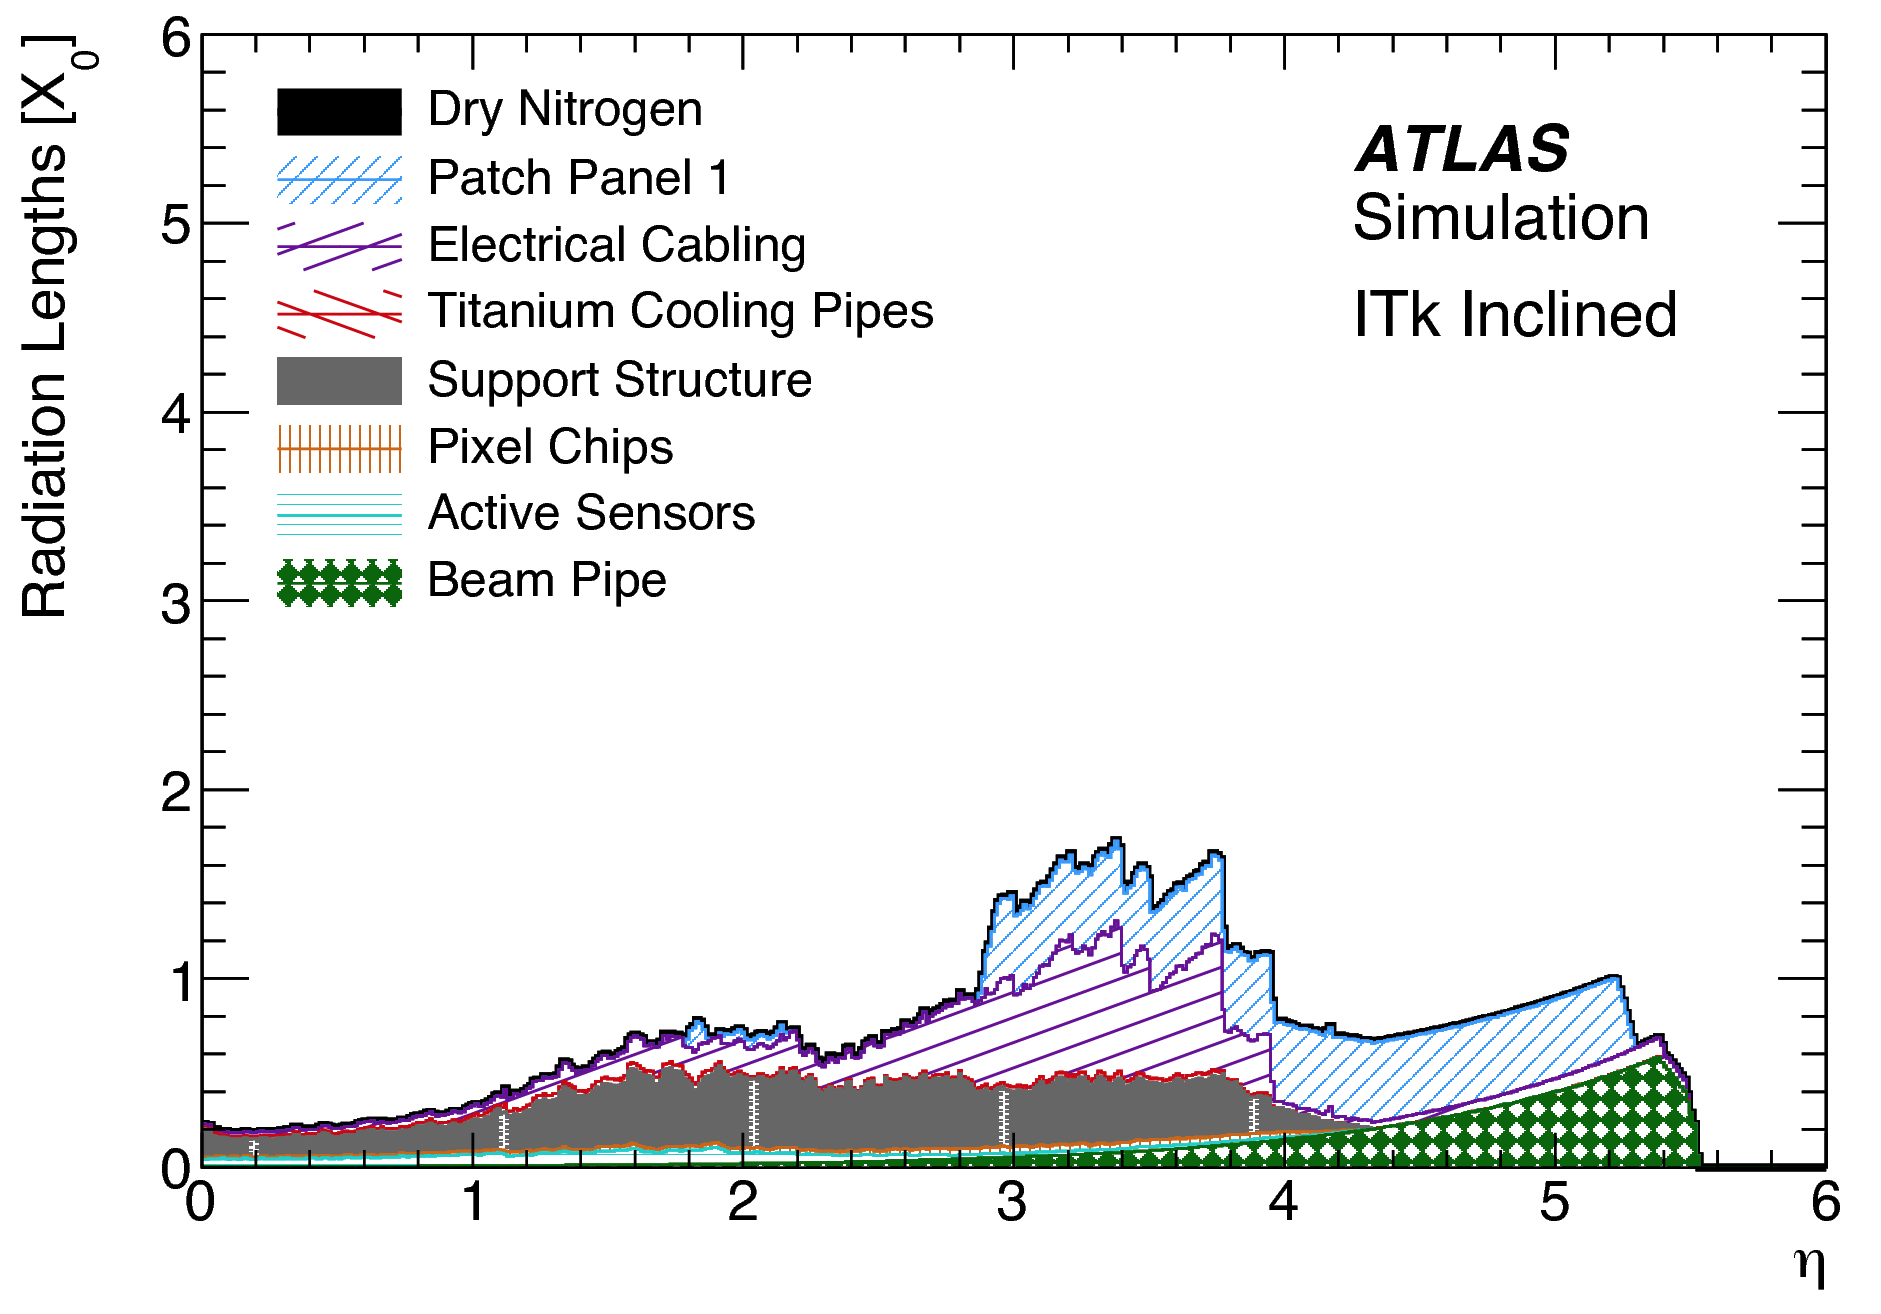
\includegraphics[width=0.49\textwidth]{ITk_X0.png}
\caption{\label{fig:ITk_X0}Material budget expressed as fraction of radiation lengths as a function of the 
pseudorapidity. (left) ATLAS ID (right) ATLAS ITk. (After~\cite{ITkStripsTDR})}
\end{figure}
  
\subsection{ITk detector layout}

The ITk will be an all silicon tracker; the main reason for abandoning the TRT is the projected occupancy 
in its straw tubes, which is about 100\% at $L=5.0\times10^{34}$cm$^{-2}$s$^{-1}$. 
The ITk will consist of an inner detector made of pixel modules and an outer one made of strips. 
In the central region of the ITk Detector, sensors are arranged in cylinders around the beam axis, with (starting from inside) five pixel layers followed by two short-strip layers of paired stereo modules then two long-strip layers of paired stereo modules. The forward regions will be covered by six strip disks and a number of pixel rings leading to one or more hits depending on the ring layer and $\eta$ position. 
The proposed ITk layout is presented in Figure~\ref{fig:ITk_Layout}. The new tracker will cover a pseudorapidity range down to $|\eta|=4$. 

\begin{figure}[!htpb]
\centering
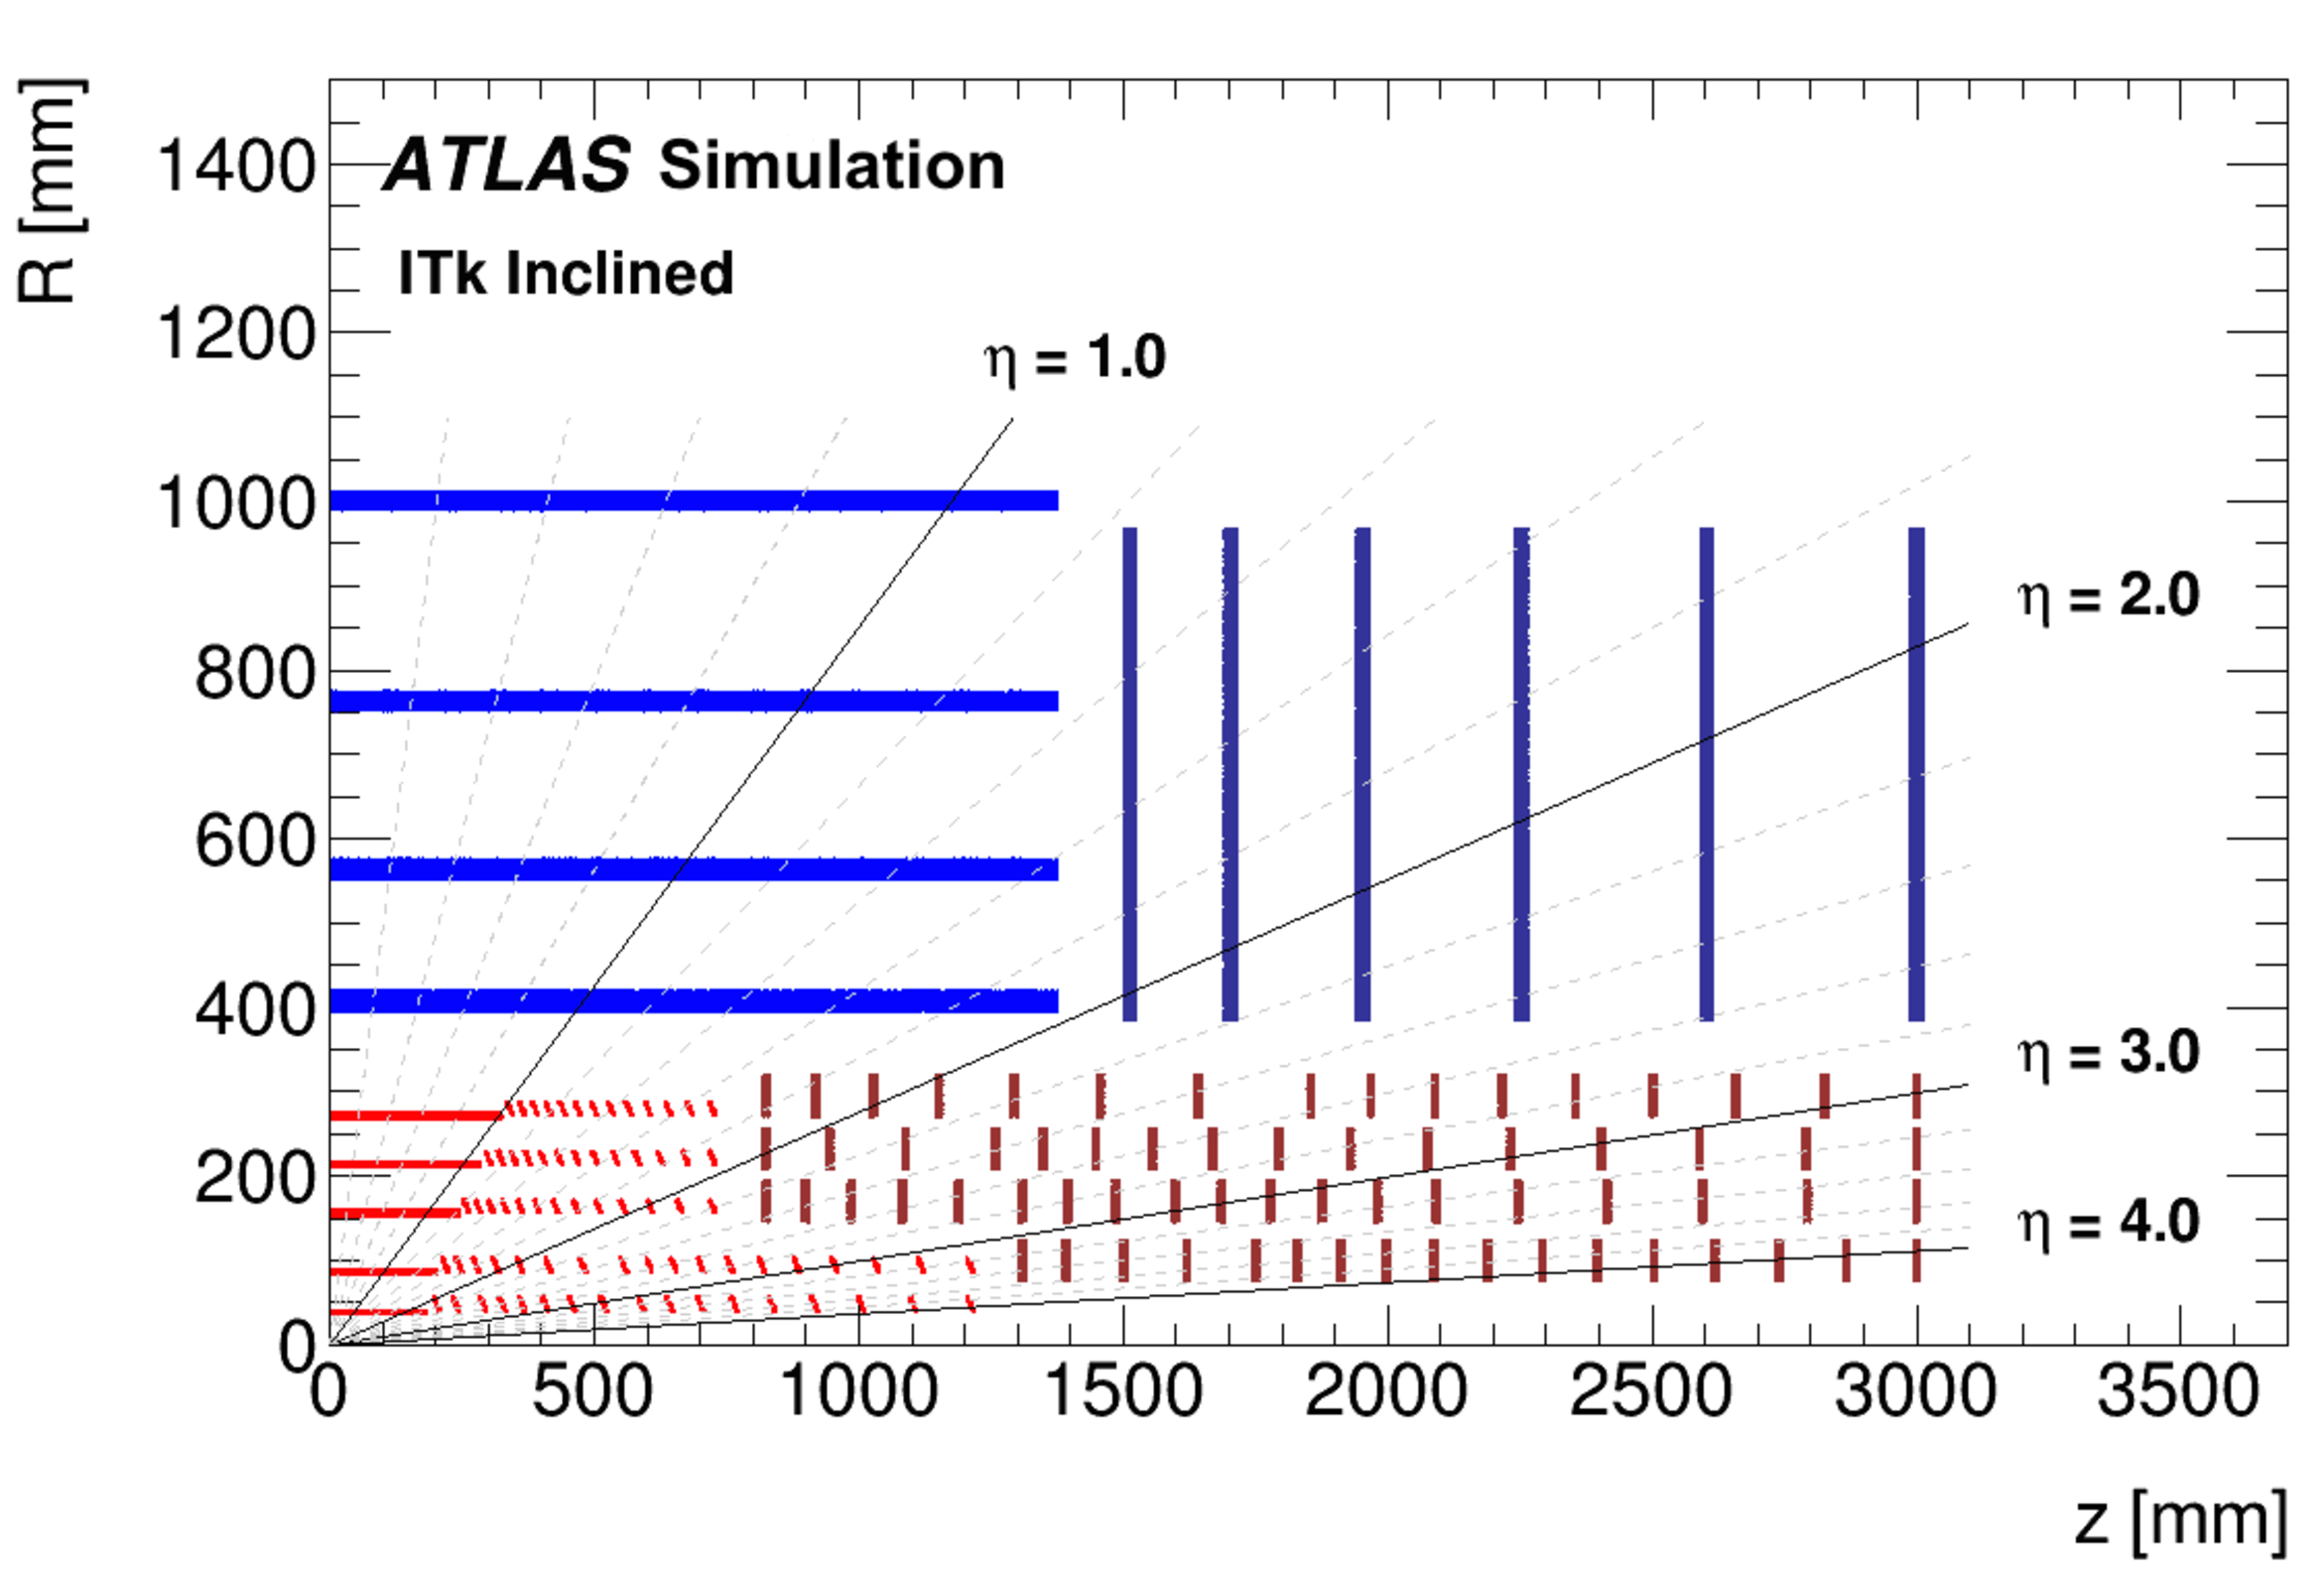
\includegraphics[width=0.65\textwidth]{ITk_Layout.pdf}
\caption{\label{fig:ITk_Layout}Schematic layout of the ITk for the HL-LHC phase of ATLAS. Here only one quadrant and only active detector elements are shown. The horizontal axis is the axis along the beam line with zero being the interaction point. The vertical axis is the radius measured from the interaction point. The outer radius is set by the bore of the solenoid. (After~\cite{ITkStripsTDR})}
\end{figure}

The peculiarity of the chosen ITk baseline layout, the so called ``Inclined'' layout, is the presence of 
inclined sensors in the forward part of the barrel layers; the inlined sensor hangs from  long 
barrel staves.
   This allows the material transversed by particles at 
large  $\eta$ to be minimised and at the same time requires less silicon surface to cover the full  $\eta$  
range. In addition, these inclined sensors provide two or more hits in the first layer, providing redundancy for the local track finding close to the interaction point even at large pseudorapidity.
One possible  support design of the Inclined layout is called ALPINE; a detail of the ALPINE stave 
prototype is shown in Figure~\ref{fig:ALPINE}.
\begin{figure}[!htpb]
\centering
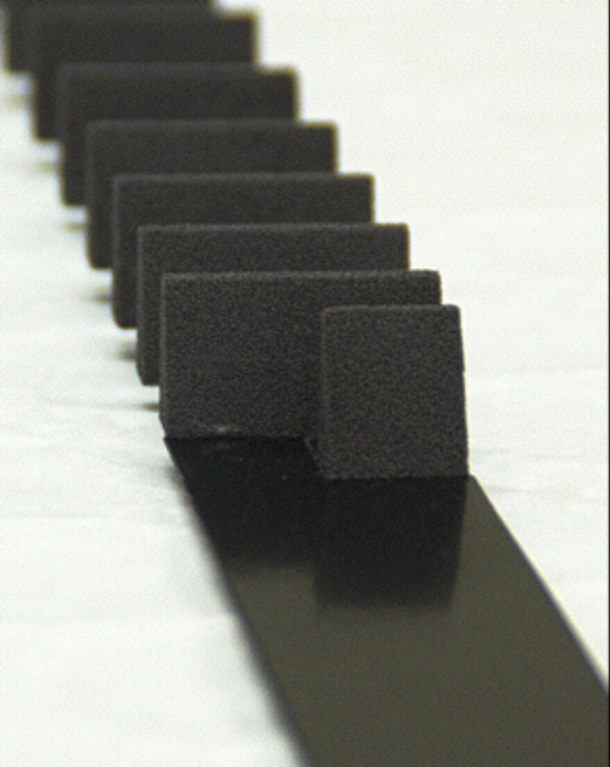
\includegraphics[height=0.25\textheight]{ALPINE.pdf}
\caption{\label{fig:ALPINE}ALPINE design for the inclined layout (After~\cite{ITkStripsTDR})}
\end{figure}
The sensor modules are located on the stave face closer to the interaction point so that incoming particles 
are detected by a pixel sensor before crossing the inactive material (local support structure, cooling tubes 
and electrical services).

\section{Pixels Detectors for ITK}
\label{sec:ITkPixels}

The innermost pixel barrel layer, Layer 0, of the ITk will be at a radius of  40~mm from the interaction 
point; the Layer 1 at 85~mm. 
Layer 2, 3 and 4 will be placed respectively at 155, 213 and 271~mm from the beam axis. 
The expected fluences for the ITk are reported in Figure~\ref{fig:ITk_Fluence}.

\begin{figure}[!htpb]
\centering
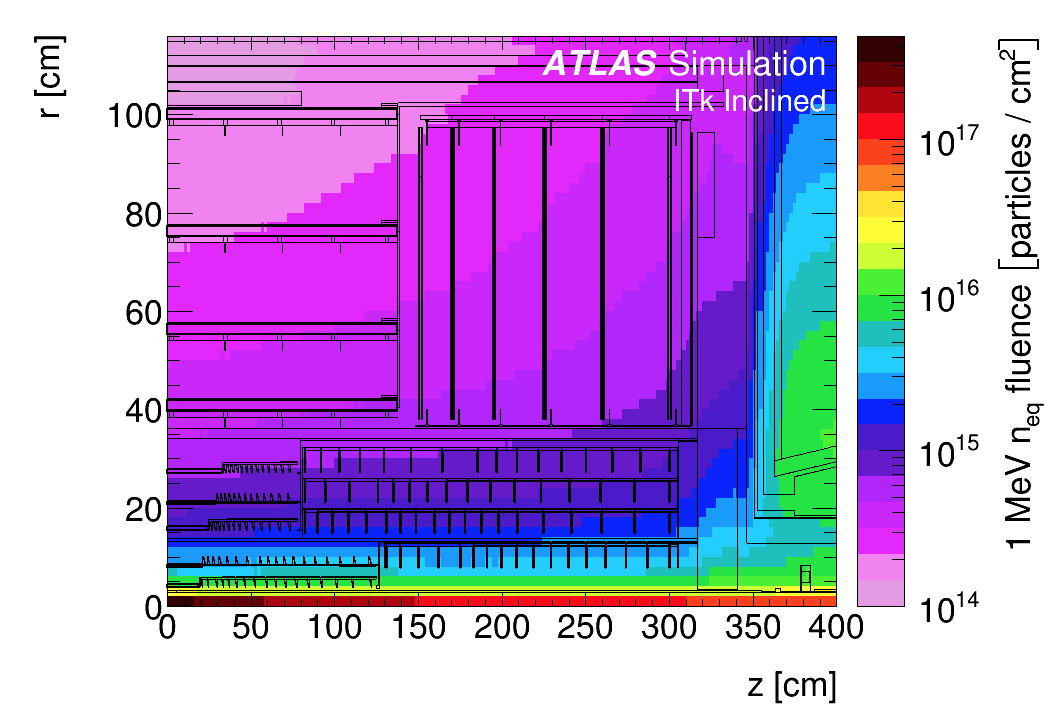
\includegraphics[width=0.65\textwidth]{ITk_Fluence.png}
\caption{\label{fig:ITk_Fluence} The 1 MeV neutron equivalent fluence  for the ITk layout 
(After~\cite{ITkStripsTDR})}
\end{figure}

The maximum fluence predicted for the Layer 0 at the end of the Phase-II program is about 1.5-2$\times10^{16}$~n$_{\rm eq}$/cm$^2$; for the pixel end-cap the largest fluence will be  of about 
5$\times10^{15}$~n$_{\rm eq}$/cm$^2$, similar to what it is expected for the Layer 1 of the barrel section.

Pixels will have a smaller pitch than today ATLAS pixel and IBL detectors; this is mandatory to keep  the 
occupancy below 1\%, in order to assure a good two particle separation and limit dead time. 
The proposed ITk layouts are designed to meet this requirement, thus the pixel pitches 
are dictated by this constraint. 
Moreover physics and performance simulations indicated that   50~$\mu$m~$\times$~50~$\mu$m pitch 
pixels, or 25~$\mu$m~$\times$~100~$\mu$m are suited (the smaller pitch is to achieve better 
momentum resolution).
Small pixel cells imply also less leakage current fed into and small capacitance coupled to the front end 
electronics, hence less noise. 


The basic  unit of the ITk pixel detector is a module. The baseline module concept for the ITk pixel detector is the well proven hybrid pixel detector in which modules are composed of a sensor and the read-out chip (ROIC) bump bonded to each other on a pixel level. In addition other concepts are also investigated such as monolithic CMOS pixel detectors, especially for the outer layers.





The choice of sensors depends mainly on the requirement that the detector has to withstand the integration of an expected dataset  of 3000\invfb.  This is particularly challenging for the innermost layer, which after the high-luminosity running will have integrated, as it was said above,  an estimated fluence $\Phi$ of 1.5-2$\times10^{16}$~n$_{\rm eq}$/cm$^2$ for the innermost pixel layer. 

There will be two main types of modules: dual-modules (two chips bump bonded to a sensor, around 
4~$\times$~2~cm$^2$) for the the innermost layer to accommodate the limited space, quad-modules (four 
chips bump bonded to a sensor, around 4 $\times$~4~cm$^2$ for the outer layers and in the rings. 
The pixel read-out chip is presently under development within the RD53 collaboration~\cite{RD53}, 
which will produce an RD53 prototype chip. Following this chip an ATLAS ITk pixel chip will be developed 
using the basic blocks designed by RD53 while integrating additional functionality to meet ATLAS 
specifications.

At this stage three possible sensor types are considered for the pixels modules:

\begin{itemize}
\item planar sensors, for an hybrid detector
\item 3D sensors, again for an hybrid detector,
\item monolithic CMOS sensors
\end{itemize}

\paragraph{3D sensors}
3D silicon detectors are candidates to be used for the inner most layer(s) of the barrel pixel system and 
some of the inner end-cap rings due to their excellent radiation hardness at low operational voltages and 
moderate temperatures with low power dissipation compared to planar sensors.
The 3D sensors will be produced on either 4" or 6" high resistivity $p-$type wafers. 
The total thickness of the sensors will be 200~$\mu$m, and and the active thickness\footnote{sensors can be realised in thin high resistivity wafers bonded to thick low resistivity ones; at the end of the fabrication process the latter can be lapped, completely or not. This approach is used to realise thin planar sensors too} will be between 
150 and 200~$\mu$m, with 150~$\mu$m being the baseline. 
The 3D sensors shall be produced by etching the $p-$ and $n-$columns from the same side (single side process). At the moment the pixel geometry will have a single readout column in the centre of the pixel (1E), surrounded by four ohmic columns. Figure~\ref{fig:3D_design} shows the proposed design of the pixel 
cell for the ITk 3D pixel modules. 

\begin{figure}[!htpb]
\centering
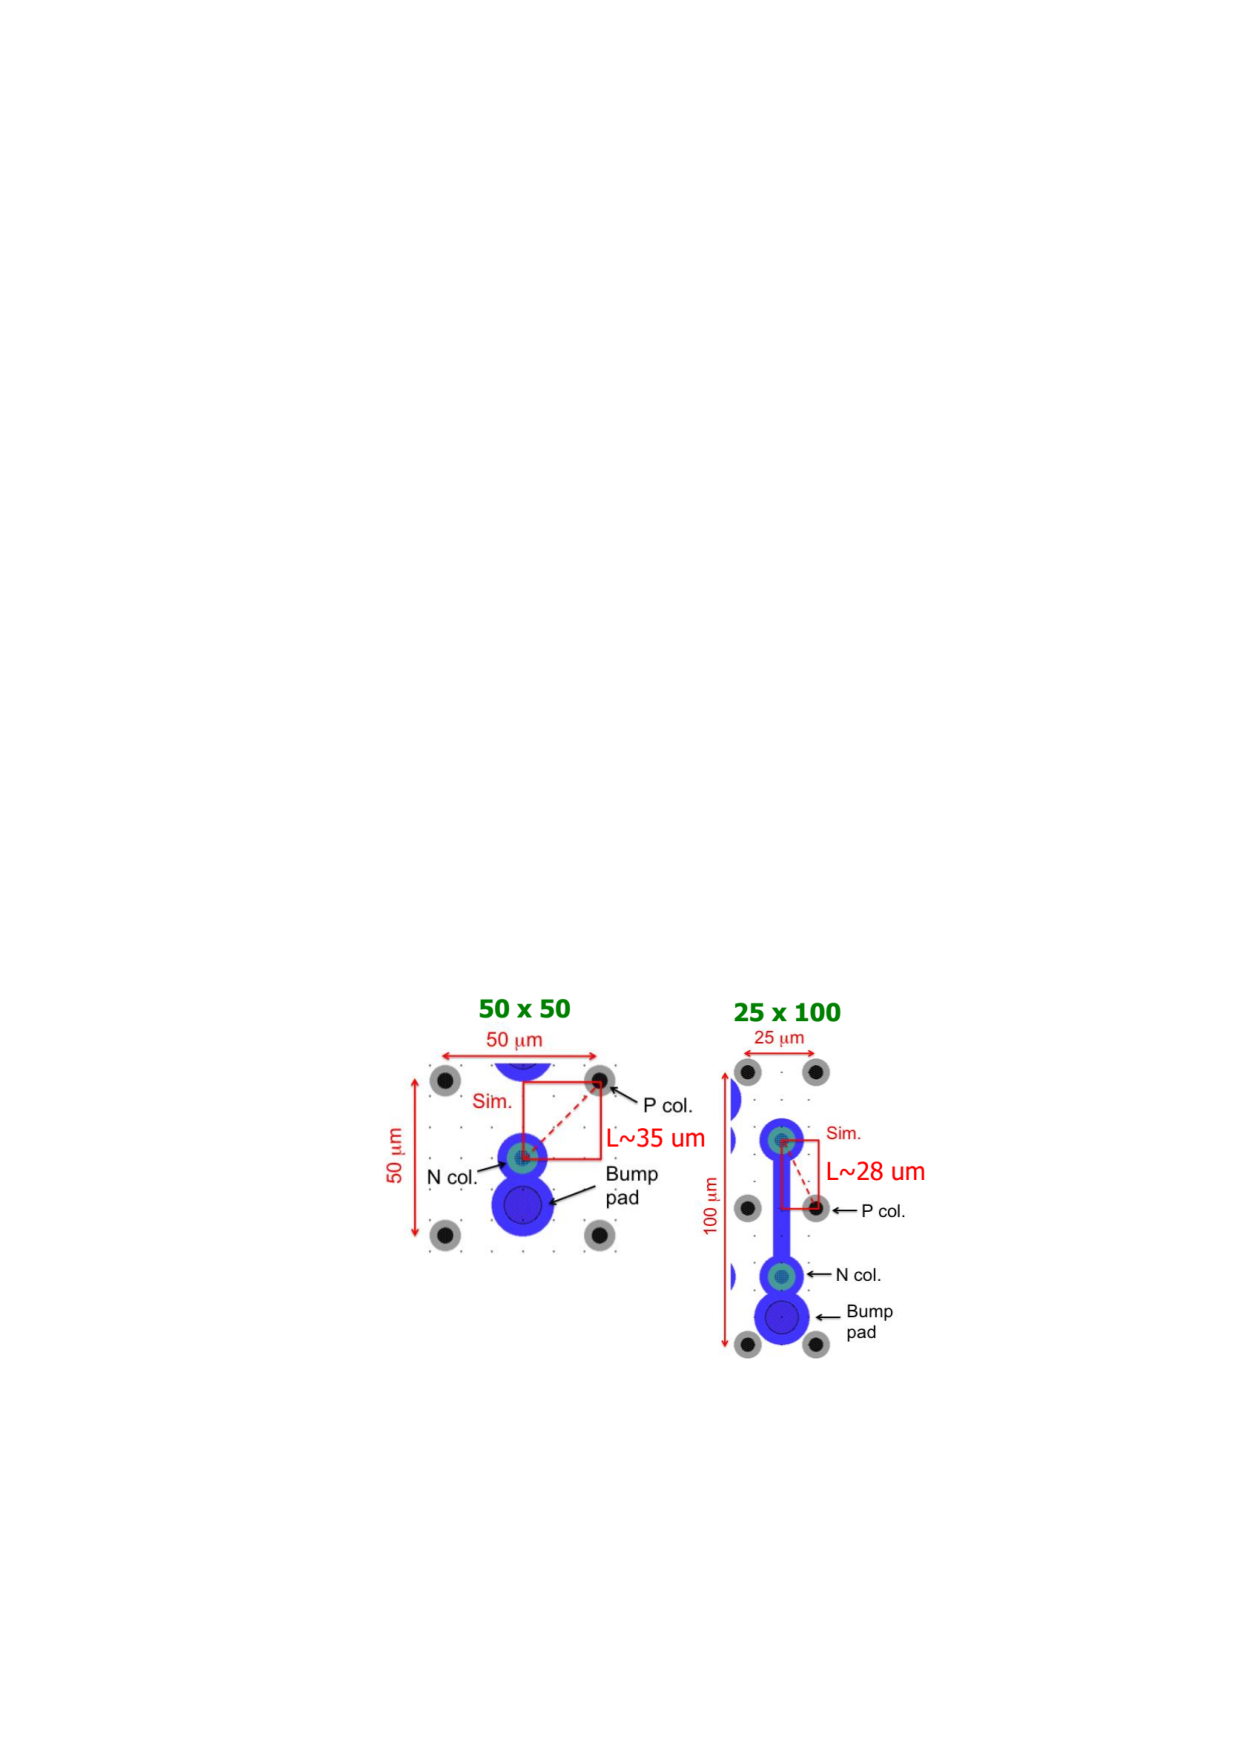
\includegraphics[width=0.55\textwidth]{3D_design.pdf}
\caption{\label{fig:3D_design} Design of 3D pixel cells with 50~$\mu$m~$\times$~50~$\mu$m  and 25~$\mu$m~$\times$~100~$\mu$m pitch pixels. (After~\cite{ITkStripsTDR})}
\end{figure}

The column diameter will be $\le$~8~$\mu$m, while the depth of the junction (ohmic) columns will be 
slightly shorter (longer) than the nominal  150~$\mu$m active thickness. Thus ohmic columns will 
be in contact with the sensor backside, while junction columns termination will be away from it, to 
avoid too early junction break down.

IBL-generation 3D pixel detectors coupled to FE-I4 pixel electronics have been found to have hit efficiencies 
in test beam measurements larger than 97\% at 170 V after irradiation to $\Phi$ of 
1.0$\times10^{16}$~n$_{\rm eq}$/cm$^2$ for normally incident minimum ionizing particles with a power 
dissipation of 15 mW/cm$^2$ at a temperature of -25$^{\circ}$~C~\cite{1748-0221-11-11-C11024}.

\paragraph{Planar sensors}
In this Paragraph only a short description of the planar sensors specification and performance 
for the ITk will be given as they will be discussed more in depth in the next two Sections. 
A new generation of planar pixel sensors are under development for the ATLAS ITk pixel system. The main 
differences with respect to the planar sensors implemented in the present detector are the different 
electrode arrangement ($n-on-p$ versus the traditional $n-on-n$) and the reduced thickness in the range of 
100-150~$\mu$m with respect to the 200~$\mu$m for the sensors used in IBL and 250~$\mu$m 
in the three outer ATLAS pixel layers. 

The $n-on-p$ technology allows for cost reduction given the single side processing and the reduced 
complexity in handling and testing. The guard ring structure is implemented on the front side, leaving the 
edges of the sensor at a potential close to the one of the backside. This arrangement potentially induces the 
risk of electrical sparks between the sensor periphery and the chip. Isolation techniques, like the deposition 
of a layer of Benzocyclobutene (BCB) on the sensor surface at wafer level or of parylene after module 
	assembly have been successfully employed to prevent this problem~\cite{Stefano,UNNO201372}.

\paragraph{Monolithic CMOS sensors}
Recent developments of CMOS pixel detectors, originally designed for charge collection in an epitaxial layer 
of 10-20~$\mu$m thickness, use new approaches to cope with the rate and radiation environment expected 
at the HL-LHC~\cite{PERIC2007876,1748-0221-11-02-C02045,HEMPEREK20158} 
based on the following enabling technology features:
HV add-ons that allow to use high depletion voltages; high resistivity wafers for large depletion depths; 
radiation hard processed with multiple nested wells to allow CMOS electronics embedded with sufficient 
shielding into the sensor substrate; and backside processing and
thinning for material minimisation and backside voltage application.

A typical CMOS sensor pixel cell with sensing substrate and a CMOS electronics layer
embedded in multiple cells is shown in Figure~\ref{fig:DMAPS}.

\begin{figure}[!htbp]
   \centering
   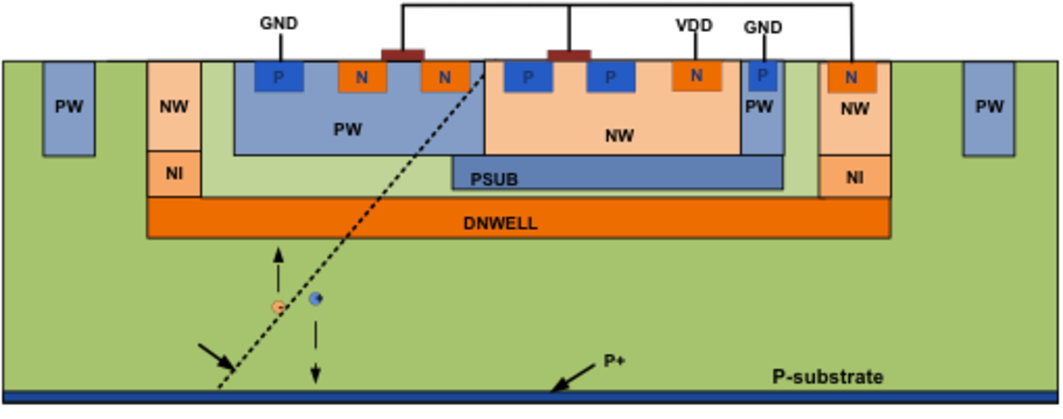
\includegraphics[width=0.65\textwidth]{DMAPS.pdf} 
   \caption{\label{fig:DMAPS}DMAPS schematic showing fully or partially depleted bulk, multiple nested wells for CMOS electronics and charge collection node. (After~\cite{ITkStripsTDR})}
   \end{figure}

Since 2014 a demonstrator programme is carried on, to prove 
DMAPS that are suited for high rate and high radiation 
operation at LHC. For this a number of technologies have been explored and characterised 
(AMS 350 nm and 180 nm, Global Foundry 130 nm, ESPROS 150 nm, LFoundry 130nm, TowerJazz 
180nm, etc.); the designs have been characterised as stand-alone sensors as well as bonded to the FE-I4 
pixel chip (as a hybrid) either via bump bonds or via glue bonding (capacitively coupled pixel detector, 
CCPD).

The results within the demonstrator programme can be summarised as follows:
\begin{itemize}
\item Technologies complying with the above list of enabling technology are principally suited to fabricate depleted monolithic sensors that can cope with the HL-LHC running condition, at least at distances larger than 20-25~cm away from the interaction point (outer layers).
\item DMAPS pixel sensors detect mips with integrated efficiencies above 98\% 
and with spatial resolutions similar to those as hybrid pixels 
\item DMAPS pixel sensors can stand radiation fluences of more than 1.0$\times10^{15}$~n$_{\rm eq}$/cm$^2$ when properly designed. This is demonstrated in Figure~\ref{fig:Eff_DMAPS} showing the 
collection width obtained after irradiation to a neutron fluence of 8.0$\times10^{15}$~n$_{\rm eq}$/cm$^2$ 
determined using
edge TCT measurements~\cite{1748-0221-12-02-P02021,5402213}.
\item  Beam test measurements have shown high rate capability as detectors bonded to the FE-I4 chip.
\item Fully monolithic DMAPS pixel sensors have been designed incorporating read-out architectures suitable to cope with the expected rates at the HL-LHC (such as column- drain architectures and direct hit transfer architectures). Such designs have been submitted for fabrication in 2016 and are currently being evaluated.
\end{itemize}

\begin{figure}[!htbp]
   \centering
   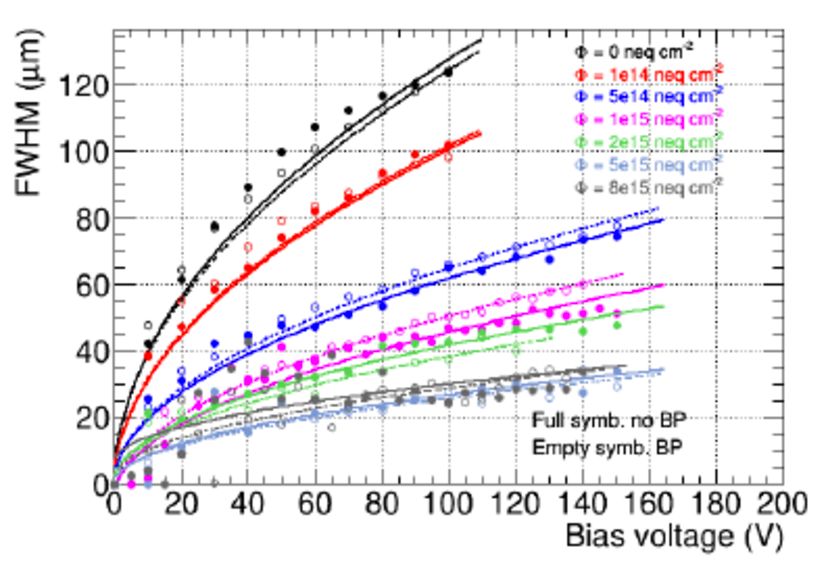
\includegraphics[width=0.6\textwidth]{Eff_DMAPS.pdf}
   \caption{\label{fig:Eff_DMAPS}FWHM of the charge collection profile measures using the edge TCT 
   technique  as a function of bias voltage after 
   different irradiation fluences up to 8.0$\times10^{15}$~n$_{\rm eq}$/cm$^2$ for un-thinned detector 
   (700~$\mu$m thick) without back plane (full symbols) and 300~$\mu$m
    sample with back plane
(empty symbols). 
(After~\cite{1748-0221-12-02-P02021})}
\end{figure}

\section{Radiation Hard Planar Pixel Sensors}
\label{sec:radhardpixels}

The ATLAS Upgrade Planar Pixel Sensor (PPS) R\&D Project~\cite{PPS:proj} carried out the optimisation of the 
well-known technology of planar silicon pixel sensors for the Phase-II of the ATLAS experiment. 
The PPS R\&D project existed from 2009 to 2014 and investigated the radiation hardness of 
pixels sensors realised in planar technology. The main research directions were: optimisation 
of the $n-$bulk material; exploration of $p-$bulk sensors; reduction of thickness; novel biasing 
structures.  
Reduction of the dead are at the detector periphery was investigated too, and it will be discussed in the 
next Section. 
These efforts   continued then within the ITk pixel forming collaboration. 

In what follows some results from the PPS activities.

\subsection{Radiation hardness of $n-on-n$ FE-I3 samples.}
In~\cite{BOMBEN2012940,1748-0221-7-10-P10028} examples of the searches within the PPS group 
are reported. Using pixel modules based on the ATLAS Pixel FE-I3 readout chip the charge collection 
efficiency (CCE) of $n-on-n$ modules was tested up to fluences 
$\Phi$=2.0$\times10^{16}$~n$_{\rm eq}$/cm$^2$. Table~\ref{tab:n-in-n} summarizes the fluences to which 
the sensors were irradiated.

\begin{table}[!htb]
\caption{\label{tab:n-in-n}Summary of irradiated n-in-n samples in the testbeams. KIT stands for 25\,MeV energy proton irradiation; reactor neutrons for the TRIGA reactor~\cite{SNOJ2011136}.
}
\begin{center}
\begin{tabular}{l|c|c|l}
name & thickness ($\mu$m)  & fluence ($10^{15}$\,n$_{\rm eq}$/cm$^2$) & irradiation type\\
\hline \hline
DO6 & 285 & 0 & -- \\
DO7 & 250 & 1 & protons (KIT)  \\
DO8 & 250 & 1 & reactor neutrons  \\
DO9 & 250 & 5 & reactor neutrons \\
DO10 & 250 & 20 & reactor neutrons \\
\hline
\end{tabular}
\end{center}
\end{table} 

These modules have been evaluated in several beam tests in 2009 and 2010.
Data presented in~\cite{1748-0221-7-10-P10028}  were taken in two different periods in 2010 at the CERN 
SPS beamline H6; in both periods pion beams of 120\,GeV/c were used.
Measurements on  samples have been carried out at temperatures well
below 0$^{\circ}$~C to reduce the large leakage current from irradiated
sensors. As an example, we measured a leakage current of 24~${\rm \mu A}$
 (10~${\rm \mu A}$) for DO10 (DO9), at a bias voltage of 1200~V and at
 -47$^{\circ}$~C.

\paragraph{Hit Efficiency}

Hit efficiency was studied as a function of the bias voltage, for the
module irradiated with $5\times 10^{15} n_{eq}/cm^{2}$.
Results are in table~\ref{tab:n-eff}.

\begin{table}[!htb]
\caption{\label{tab:n-eff}Hit efficiency of an irradiated (fluence = $5\times 10^{15} n_{eq}/cm^{2}$)
FEI3 $n-on-n$ 200~$\mu$m thick module at different bias voltages.}
\begin{center}
\begin{tabular}{|c|c|c|}
\hline
Bias voltage (V) & Hit efficiency (\%) \\
\hline
350 & 93.2 \\
\hline
500 & 97.3 \\
\hline
1000 & 99.6 \\
\hline
\end{tabular}
\end{center}

\end{table}

\begin{figure}[!htb]
\begin{center}
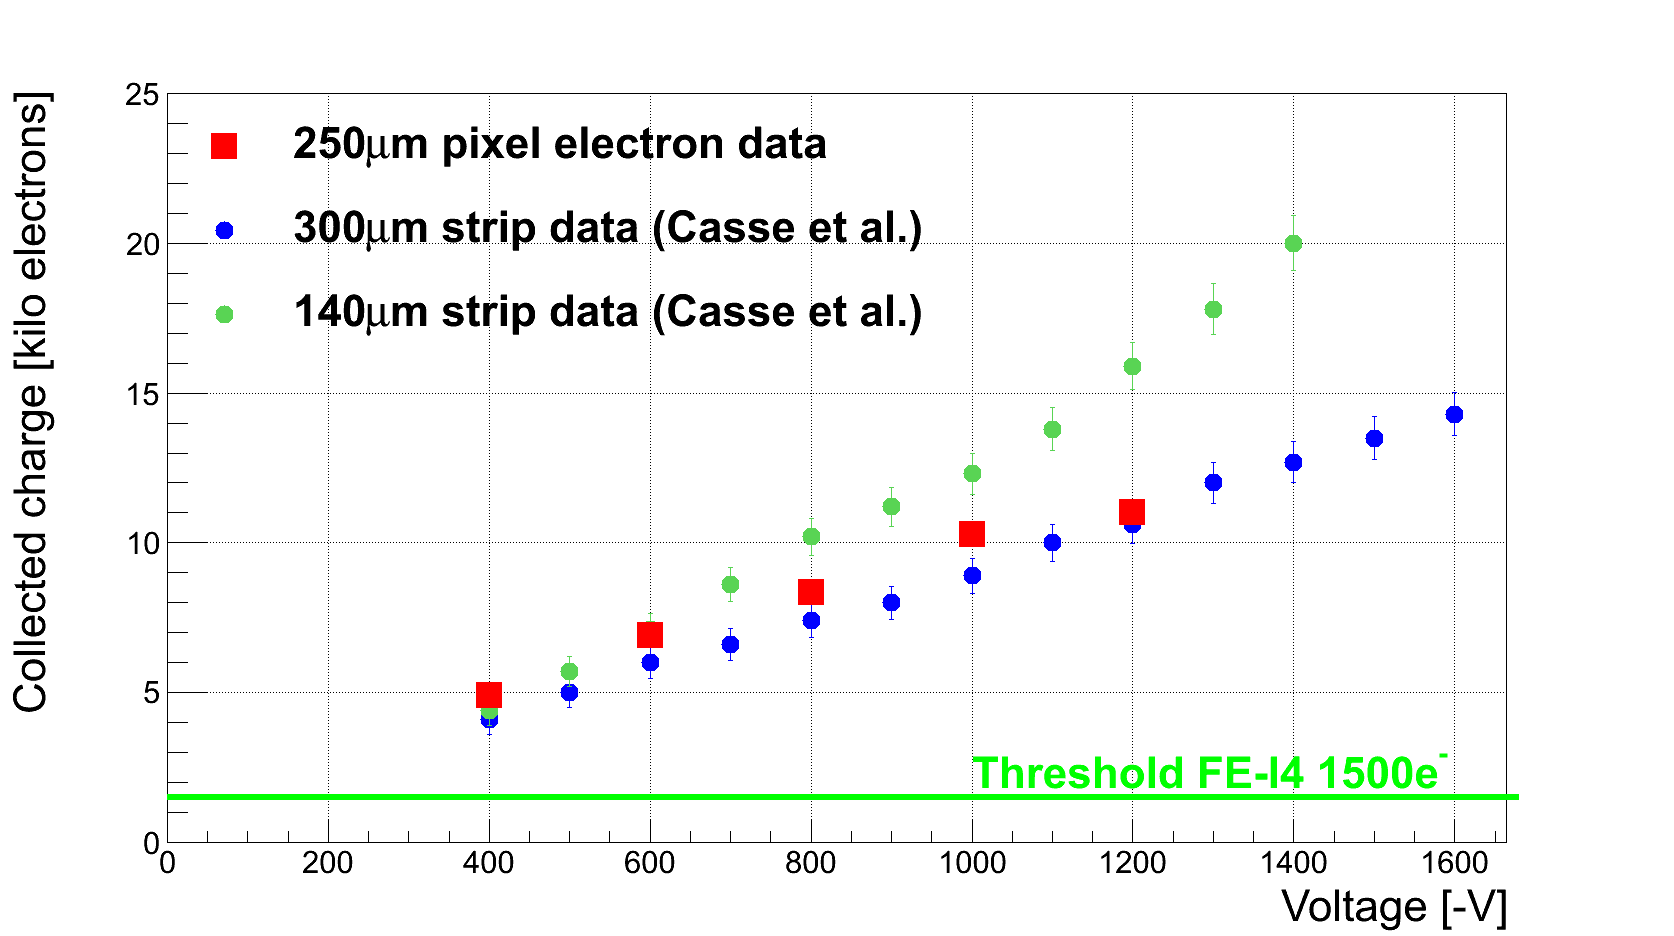
\includegraphics[width=0.49\textwidth]{5E15_onlyElectrons.png}
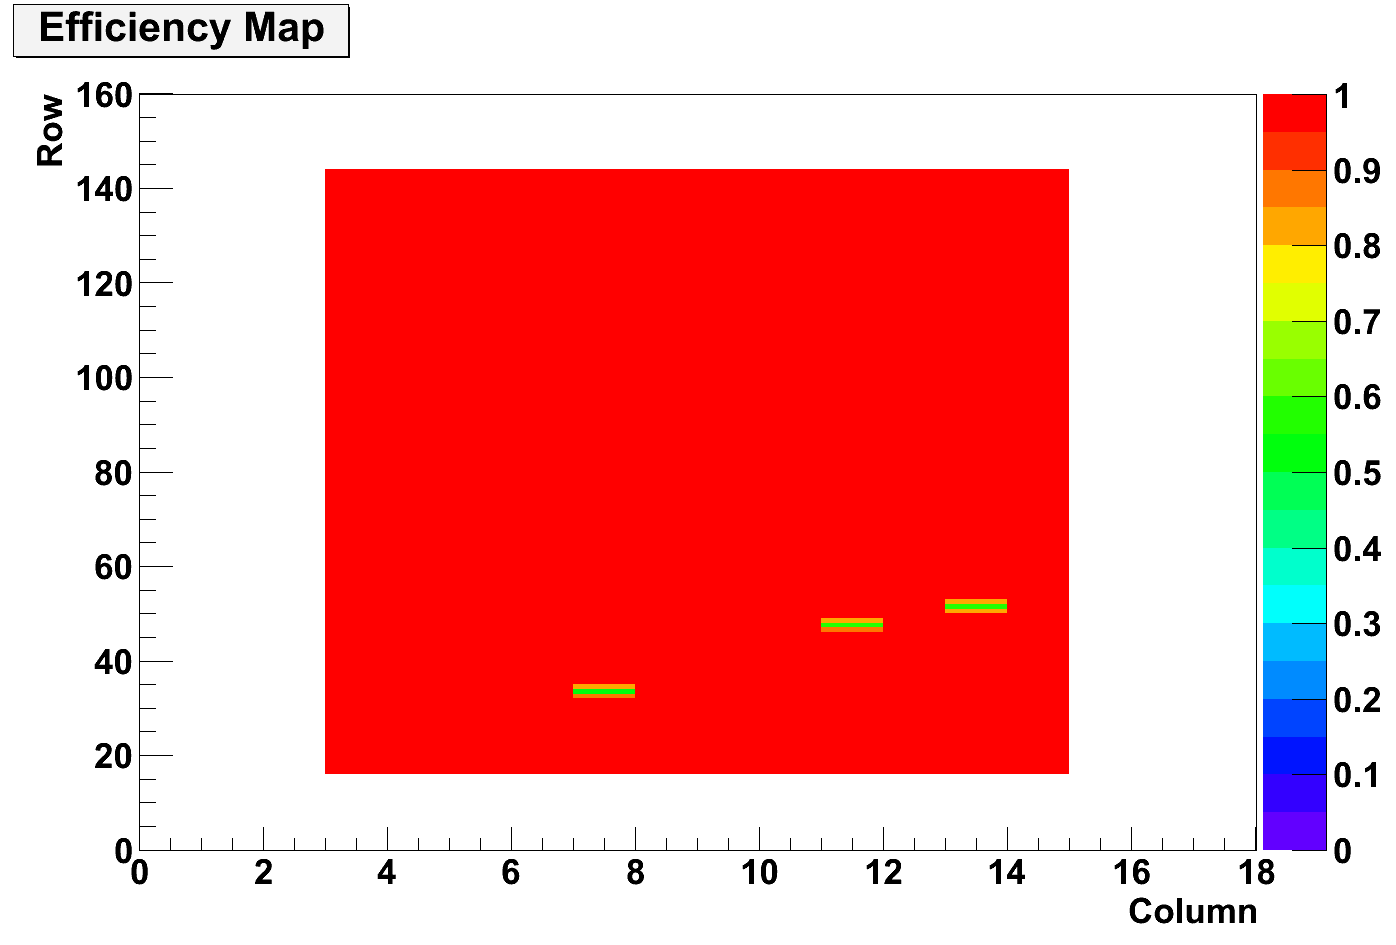
\includegraphics[width=0.44\textwidth]{EffMap_DO13_1000V.png}
\end{center}
\caption{\label{fig:5e15}left: Collected charge as a function of the bias for sensors irradiated
with fluence of $5\times 10^{15} n_{eq}/cm^{2}$; right: Hit efficiency map for the same assembly}
\end{figure}

In figure~\ref{fig:5e15}, on the left, a study of the collected charge vs bias voltage
 for a module irradiated with a fluence of $5\times 10^{15} n_{eq}/cm^{2}$ is shown\footnote{as
 a comparison data from strip detectors~\cite{Casse} are reported too.} (only data collected with the
 $^{90}$Sr  source are shown).  In the figure the expected threshold for the FE-I4
 chip is shows too. A signal of about 10 ke$^-$ is observed at 1000 V. This was very
 promising for the  ATLAS IBL~\cite{IBLTDR}, and
  the outer pixel layers at HL-LHC.

In figure~\ref{fig:5e15}, on the right, the hit-efficiency map for the module irradiated with a
fluence of $5\times 10^{15} n_{eq}/cm^{2}$, as measured at the testbeam for particles
at normal incidence. The pixel module was biased at 1000 V and the hit-efficiency was 99.6\%.


\paragraph{Charge Collection Efficiency}
One of the main effects of irradiation is the increased trapping, which leads to a reduced signal amplitude. 
As the trapping probability depends on the charge carrier velocity, the collected charge was measured as a 
function of the bias voltage. Figure~\ref{fig:DO_all_Save} shows the results for all irradiated $n-on-n$ 
samples in the two beam test periods; see also Table~\ref{tab:n-in-n}. A systematic error on the collected 
charge of 400\,e is assumed, due to the finite charge resolution of the ToT mechanism;  a 5\% systematic 
uncertainty is also taken into account, due to non-uniformity in the injection capacitances.\\
After $5\times 10^{15}$\,n$_{\rm eq}$/cm$^2$, the collected charge still exceeds 10~ke at a bias voltage of 
1000\,V. Even if the collected charge is shared equally between two neighboring pixels, this charge is 
sufficient to detect the hit with FE-I3.

\begin{figure}[!htpb]
 \begin{center}
  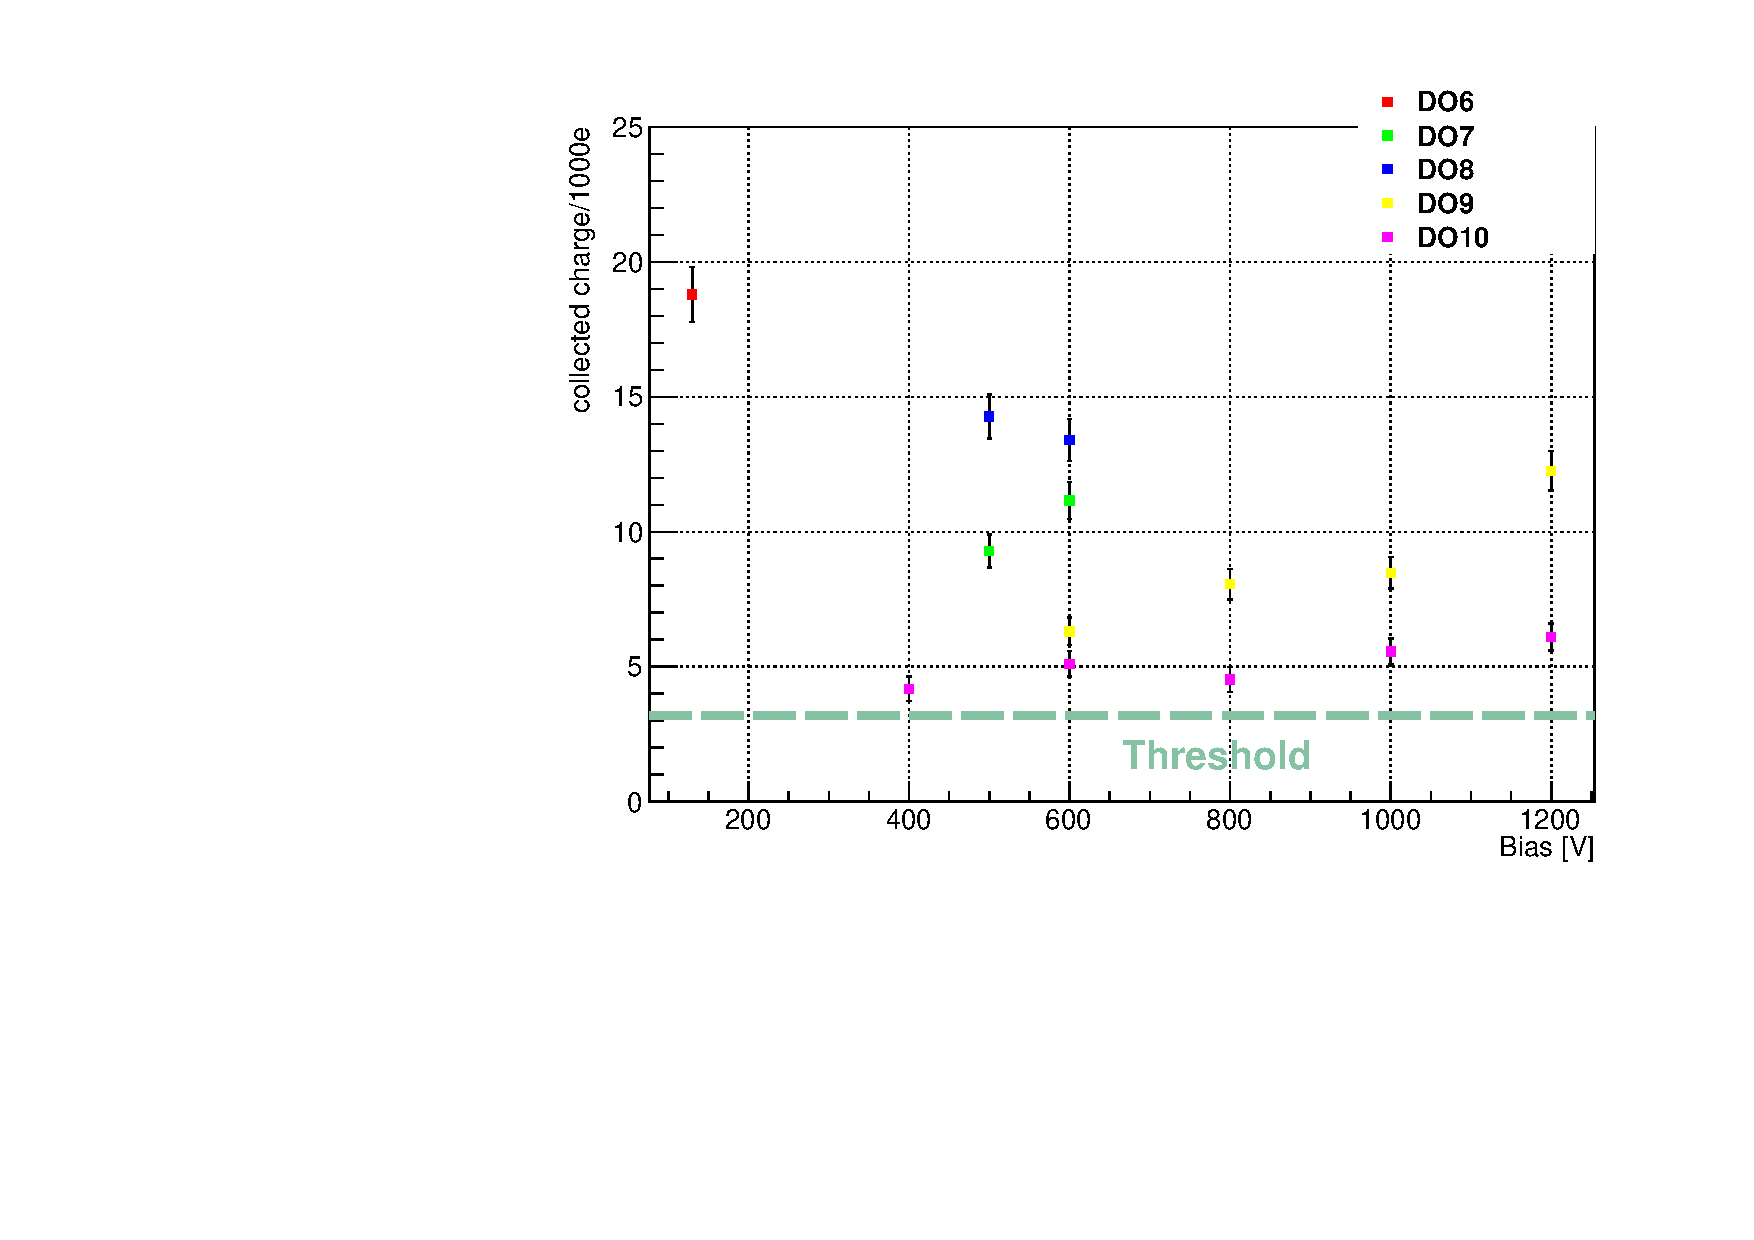
\includegraphics[width=0.65\textwidth]{DO_all_Save.pdf}
 \end{center}
 \caption{\label{fig:DO_all_Save}Collected charge as a function of bias voltage for $n-on-n$ samples irradiated to different fluences
 (see details in the text).
 A threshold of 3200~e is indicated.}
\end{figure}

Figure \ref{fig:n-in-n:Oct_P5_D11_qeff} top, shows that charge is predominantly
 lost in the region of the punch-through bias grid system.

 At very high fluences ($2\times 10^{16}$\,n$_{\rm eq}$/cm$^2$, DO10 sample)
 it is no longer possible to say which region is less efficient than the others, using the charge collection method
 (Figure \ref{fig:n-in-n:Oct_P5_D11_qeff}, bottom).
\begin{figure}[!htb]
 \begin{center}
  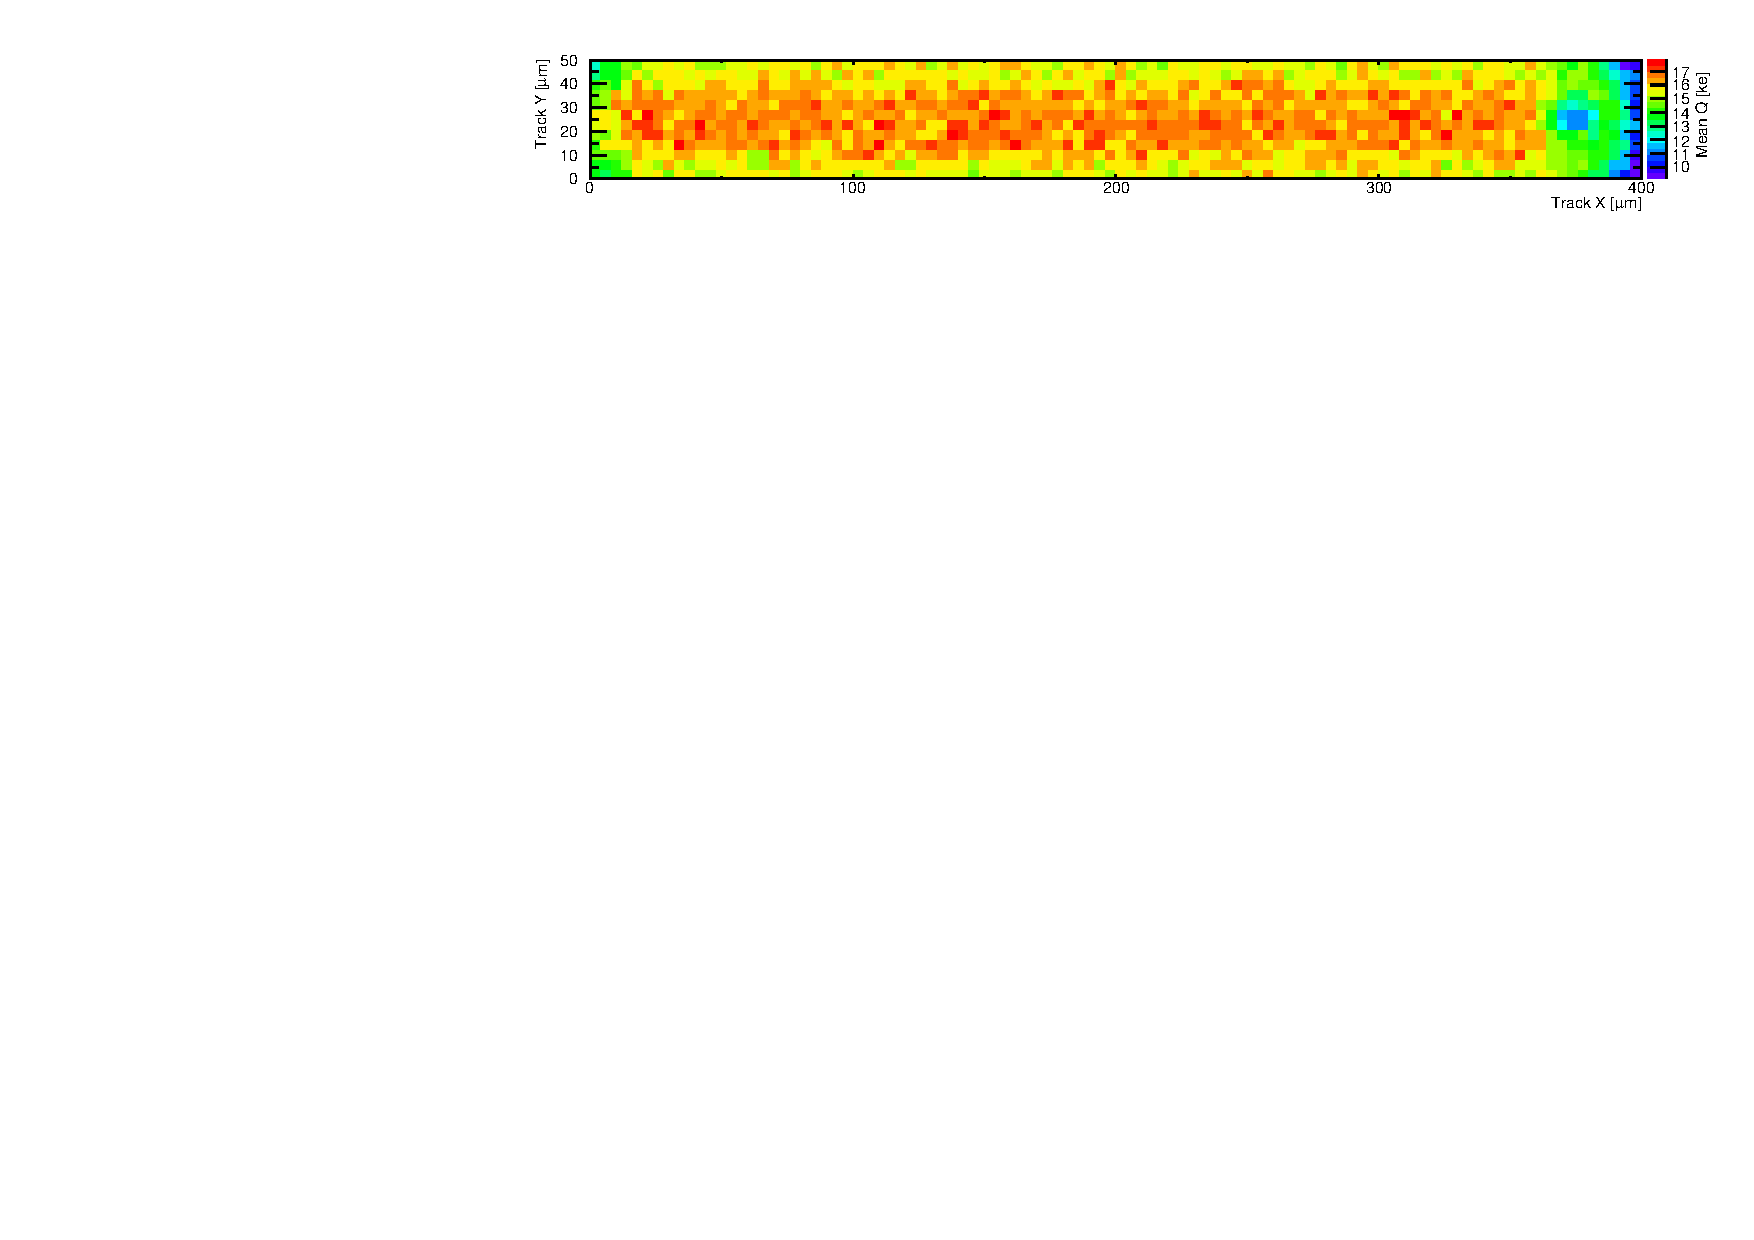
\includegraphics[width=1\textwidth]{Oct_P8_1_9_9_1_D10_qeff.pdf}
  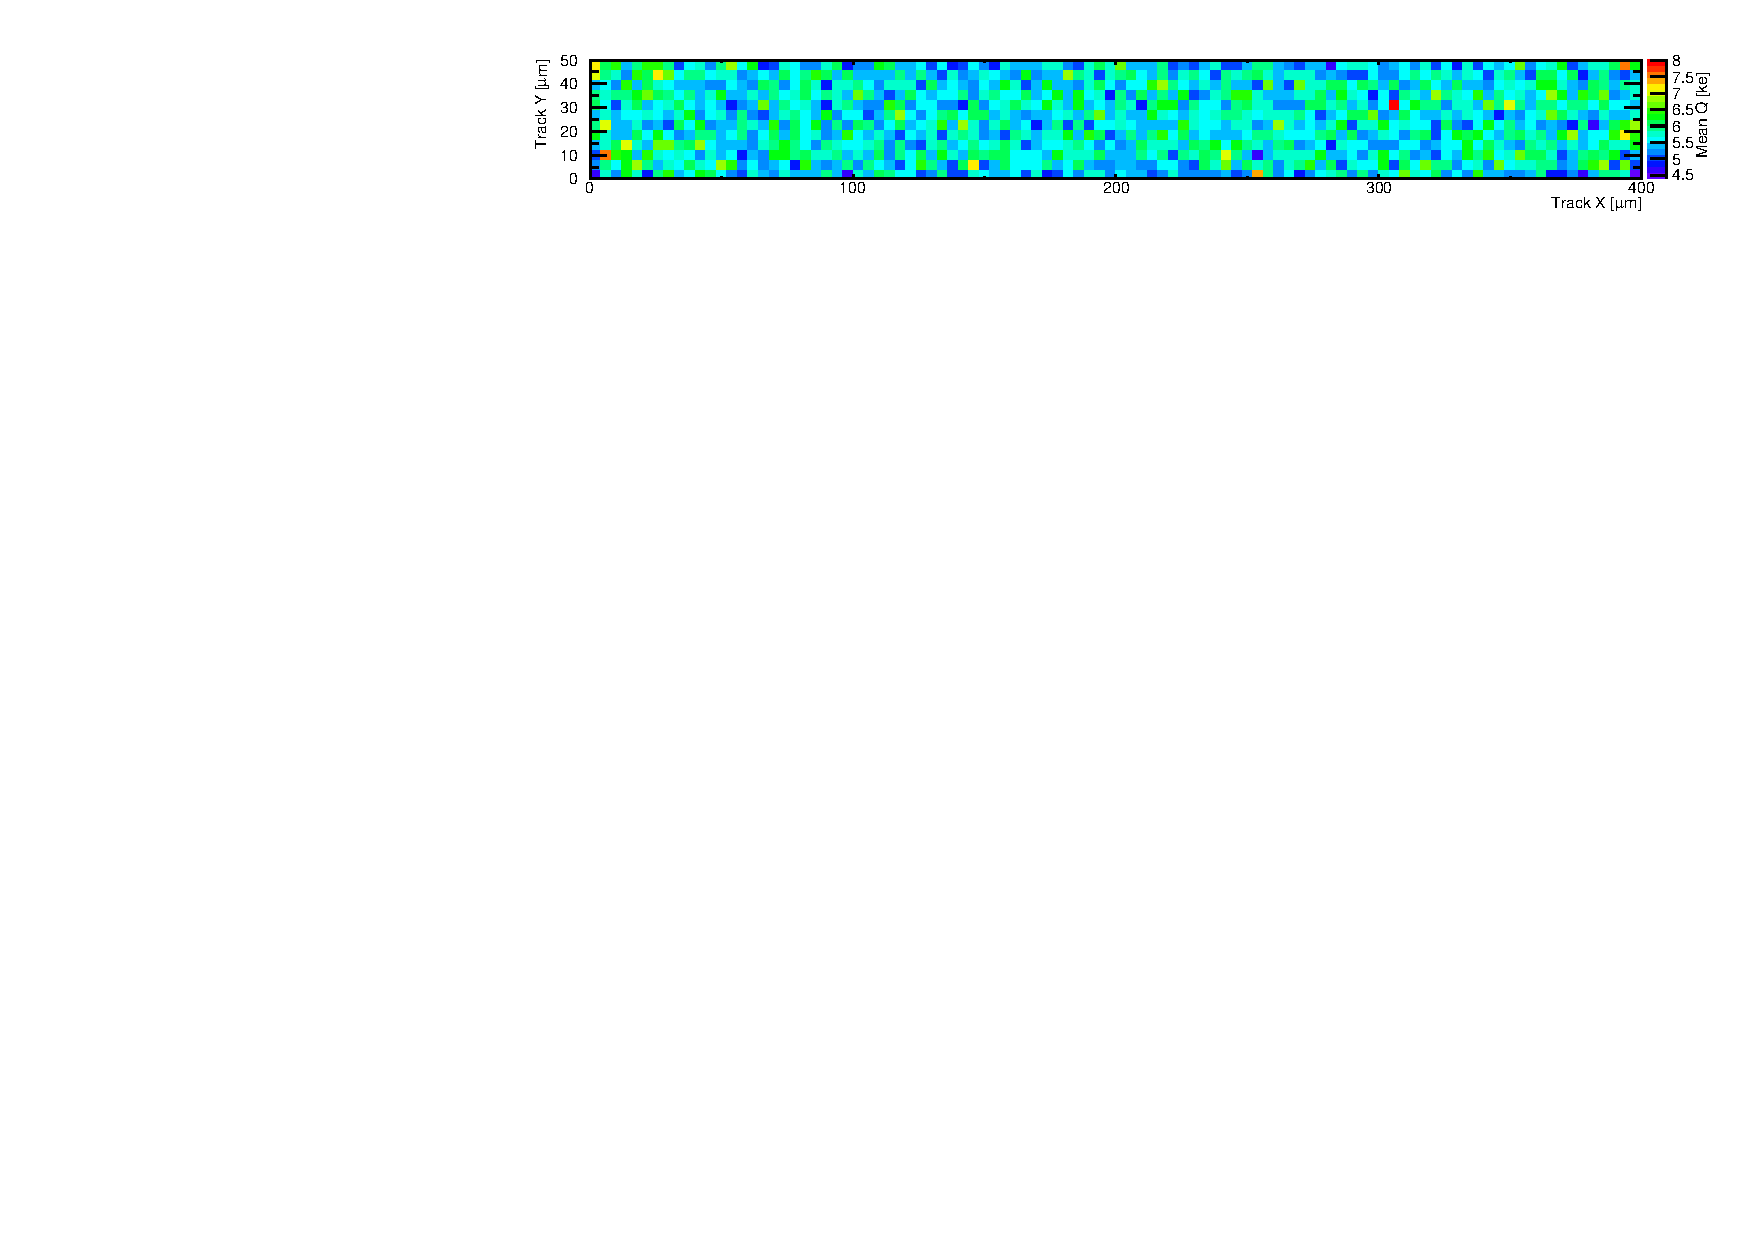
\includegraphics[width=1\textwidth]{Oct_P5_D11_qeff.pdf}
 \end{center}
 \caption{\label{fig:n-in-n:Oct_P5_D11_qeff}Charge collection within a pixel. Top: DO9 at V$_{bias}$=1200\,V. Bottom: DO10 at V$_{bias}$=1000\,V.}
\end{figure}

\paragraph{Charge Sharing Probability}

To calculate the charge sharing probability for each hit within a cluster, it is determined whether a hit is found in a pixel cell adjacent to the one matched to a track.
This probability increases towards the edge of the pixel since charge carriers are more likely to drift to the neighbouring pixel. The corresponding plot, referred to as a charge sharing map, is centred on one pixel, also showing half of the adjacent pixel in each direction.
The overall charge sharing is defined as the number of tracks with at least one hit in a neighbouring pixel divided by the number of all tracks.

Figure \ref{fig:n-in-n:DO9_qshare} shows the charge sharing probability for DO9 at a bias voltage of 1200\,V.
Reduced charge sharing probability is visible in the region of the bias dot
 and the bias grid network.\footnote{The bias grid network is an aluminum trace
 arranged on top of the intermediate pixel region connecting all bias dots.}
 Less charge is deposited here, so there is a higher probability for the second pixel in a two-pixel cluster to be below threshold.
As only the bias trace makes the difference between both pixel sides, it might cause the lower charge sharing probability. Furthermore, one can see that the region of the bias dot is not affected.

 While for DO9 a clear increase in charge sharing probability towards the edges of the pixel is visible, at higher fluence the collected charge becomes too small for any significant charge sharing to be observable. 
\begin{figure}[!htpb]
 \begin{center}
 \hspace{-.28cm}
  
\includegraphics[width=0.887\textwidth]{n_pixel_charge_share_v5_2.png}
  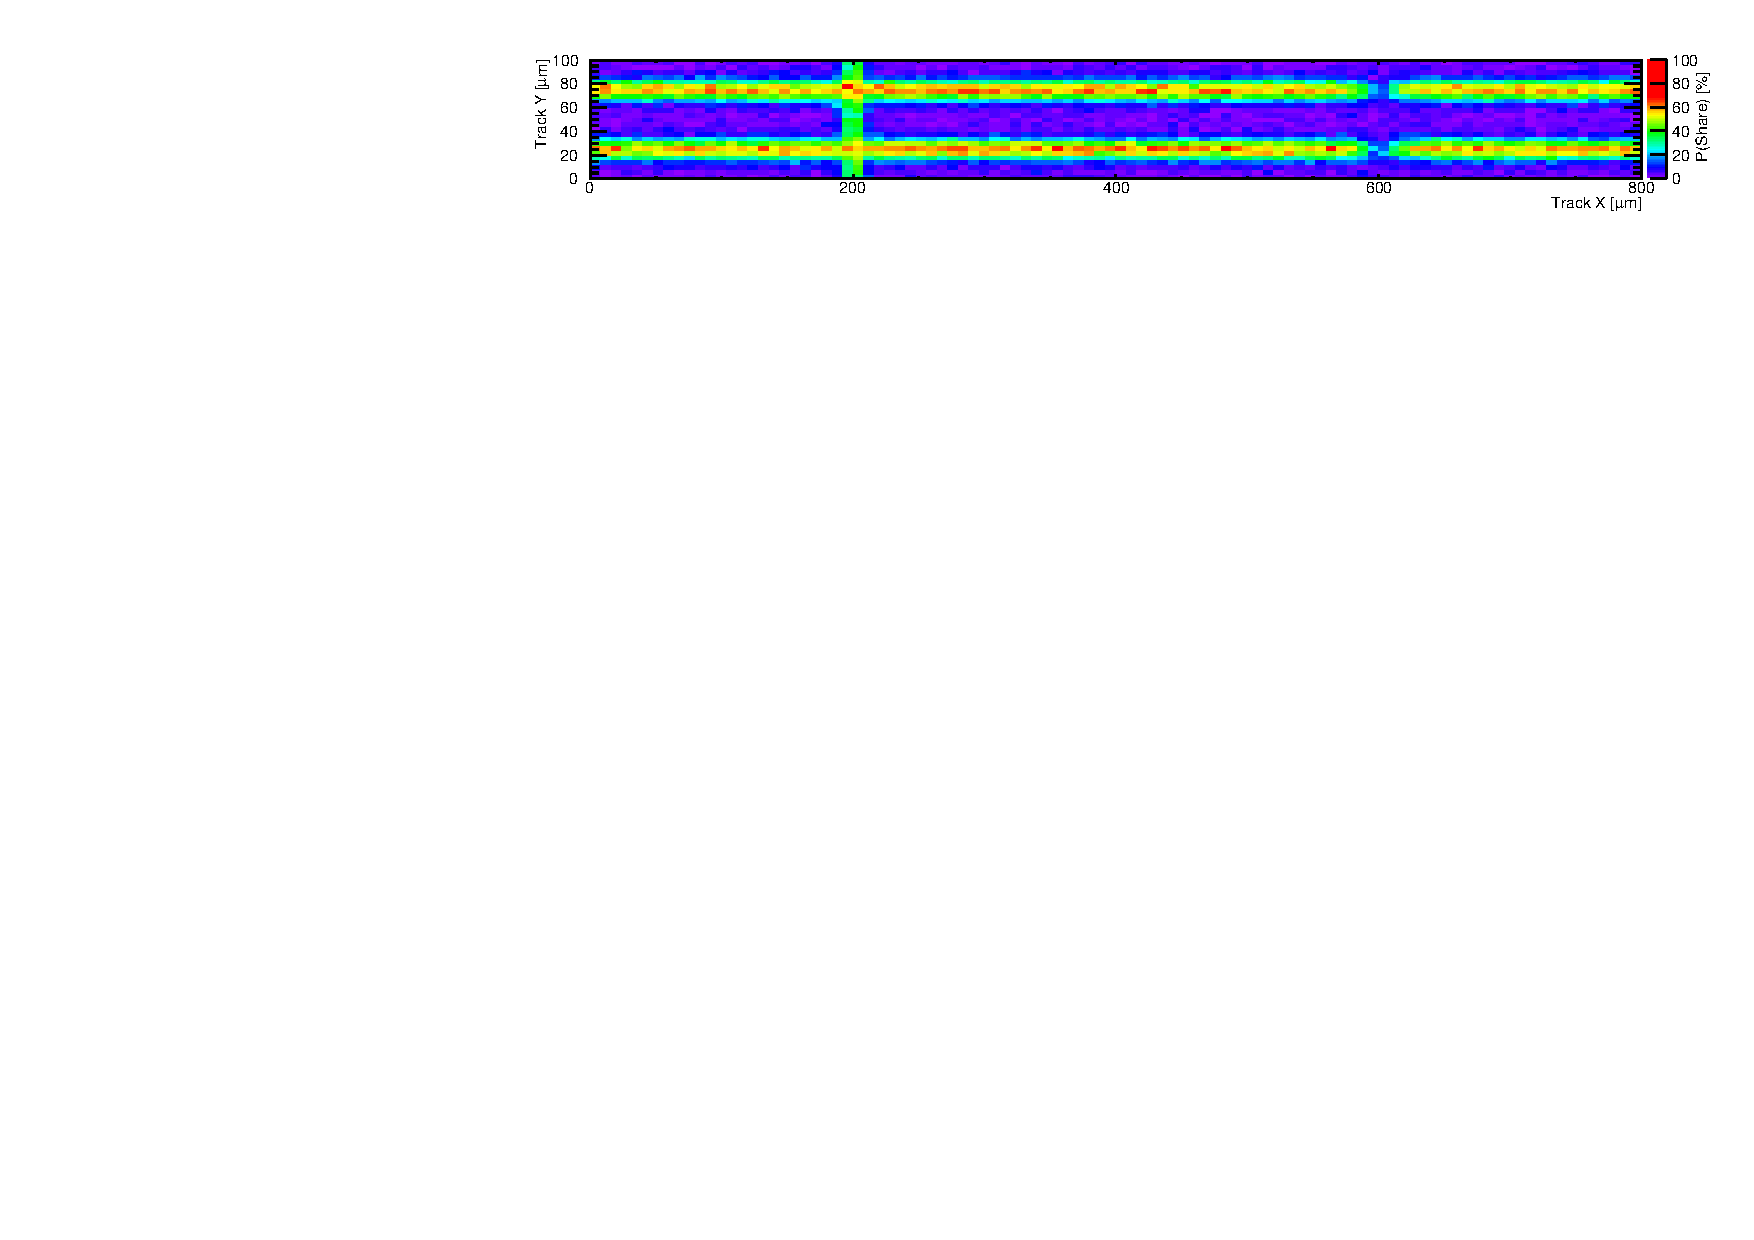
\includegraphics[width=\textwidth]{Oct_P8_1_9_9_1_D10_qshare.pdf}
 \end{center}
 \caption{Top: Design of the sample of the region shown in the plot below. Bottom: Charge sharing probability for DO9 at V$_{bias}$=1200V. Note the reduced charge sharing in the bias grid region on the right-hand side of the central pixel. \label{fig:n-in-n:DO9_qshare}}
\end{figure}

\paragraph{Residuals}
To estimate the intrinsic spatial resolution of the devices under test (DUTs),
 the distribution of hit residuals was studied. The intrinsic spatial resolution was estimated by the RMS of the 
 residual distribution for clusters of all sizes, while the residual distribution of 2-pixel clusters is used to 
 estimate the width of the area between pixels, where charge sharing occurs. The distribution is fitted with 
 the sum of two Gaussian functions, where one accounts for misreconstructed hits, resulting in large 
 residual values (equal to 2 times the pixel pitch or more), and the other for correctly reconstructed hits. The 
 width of this ``core'' Gaussian gives the width of the charge sharing region.
 
 Figure \ref{fig:n-in-n:residuals} shows the residual distributions in the 50\,$\mu$m pixel direction for the unirradiated sample (DO6) and the sample irradiated to
\mbox{$2\times10^{16}\,{\rm n_{eq}}/{\rm cm}^2$}, respectively. The widths of the distributions are 16\,$\mu$m and 15.4\,$\mu$m, comparable with the expected digital resolution of 14.4\,$\mu$m. Thus, no influence of radiation damage on the spatial resolution can be observed.

\begin{figure}[!htb]
 \begin{center}
  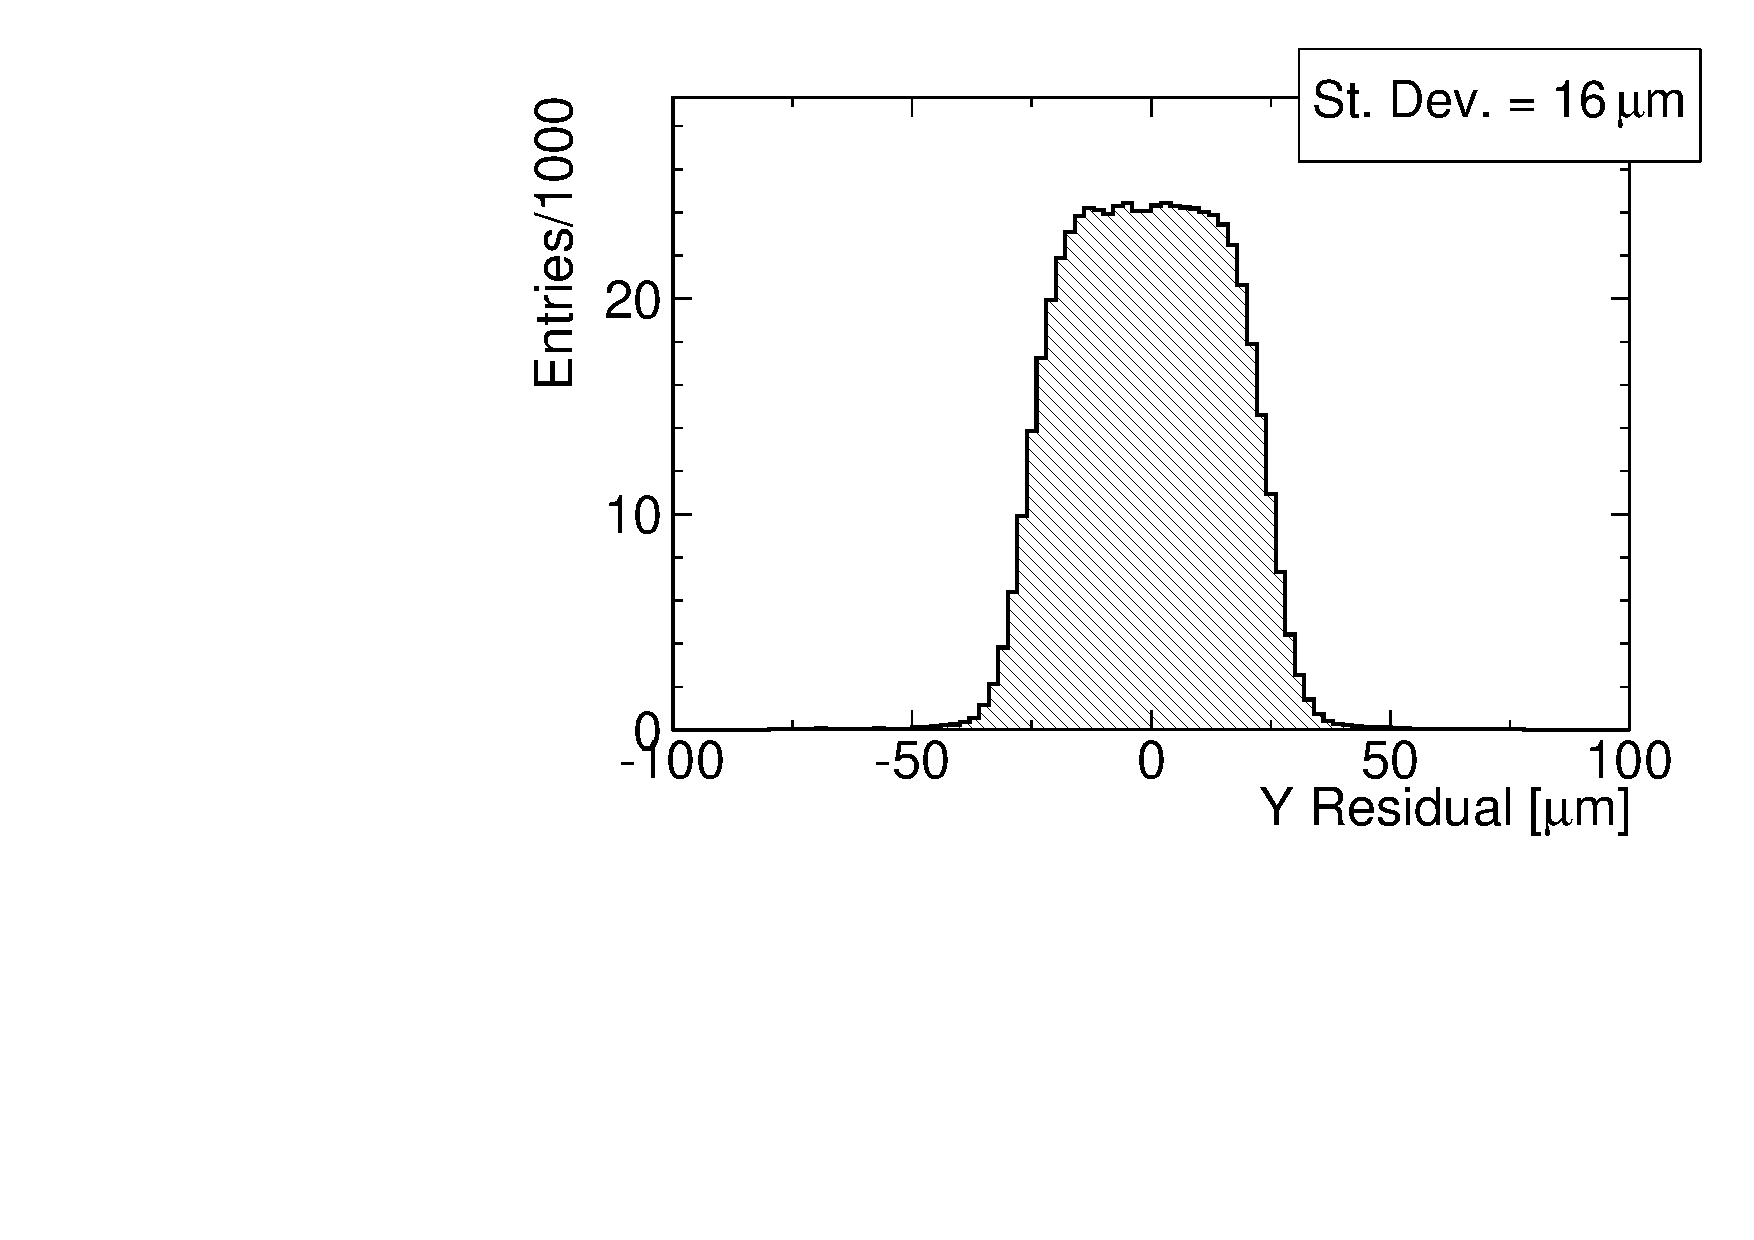
\includegraphics[width=.49\textwidth]{Oct_Period1-residuals2-11-fitResY.pdf}
  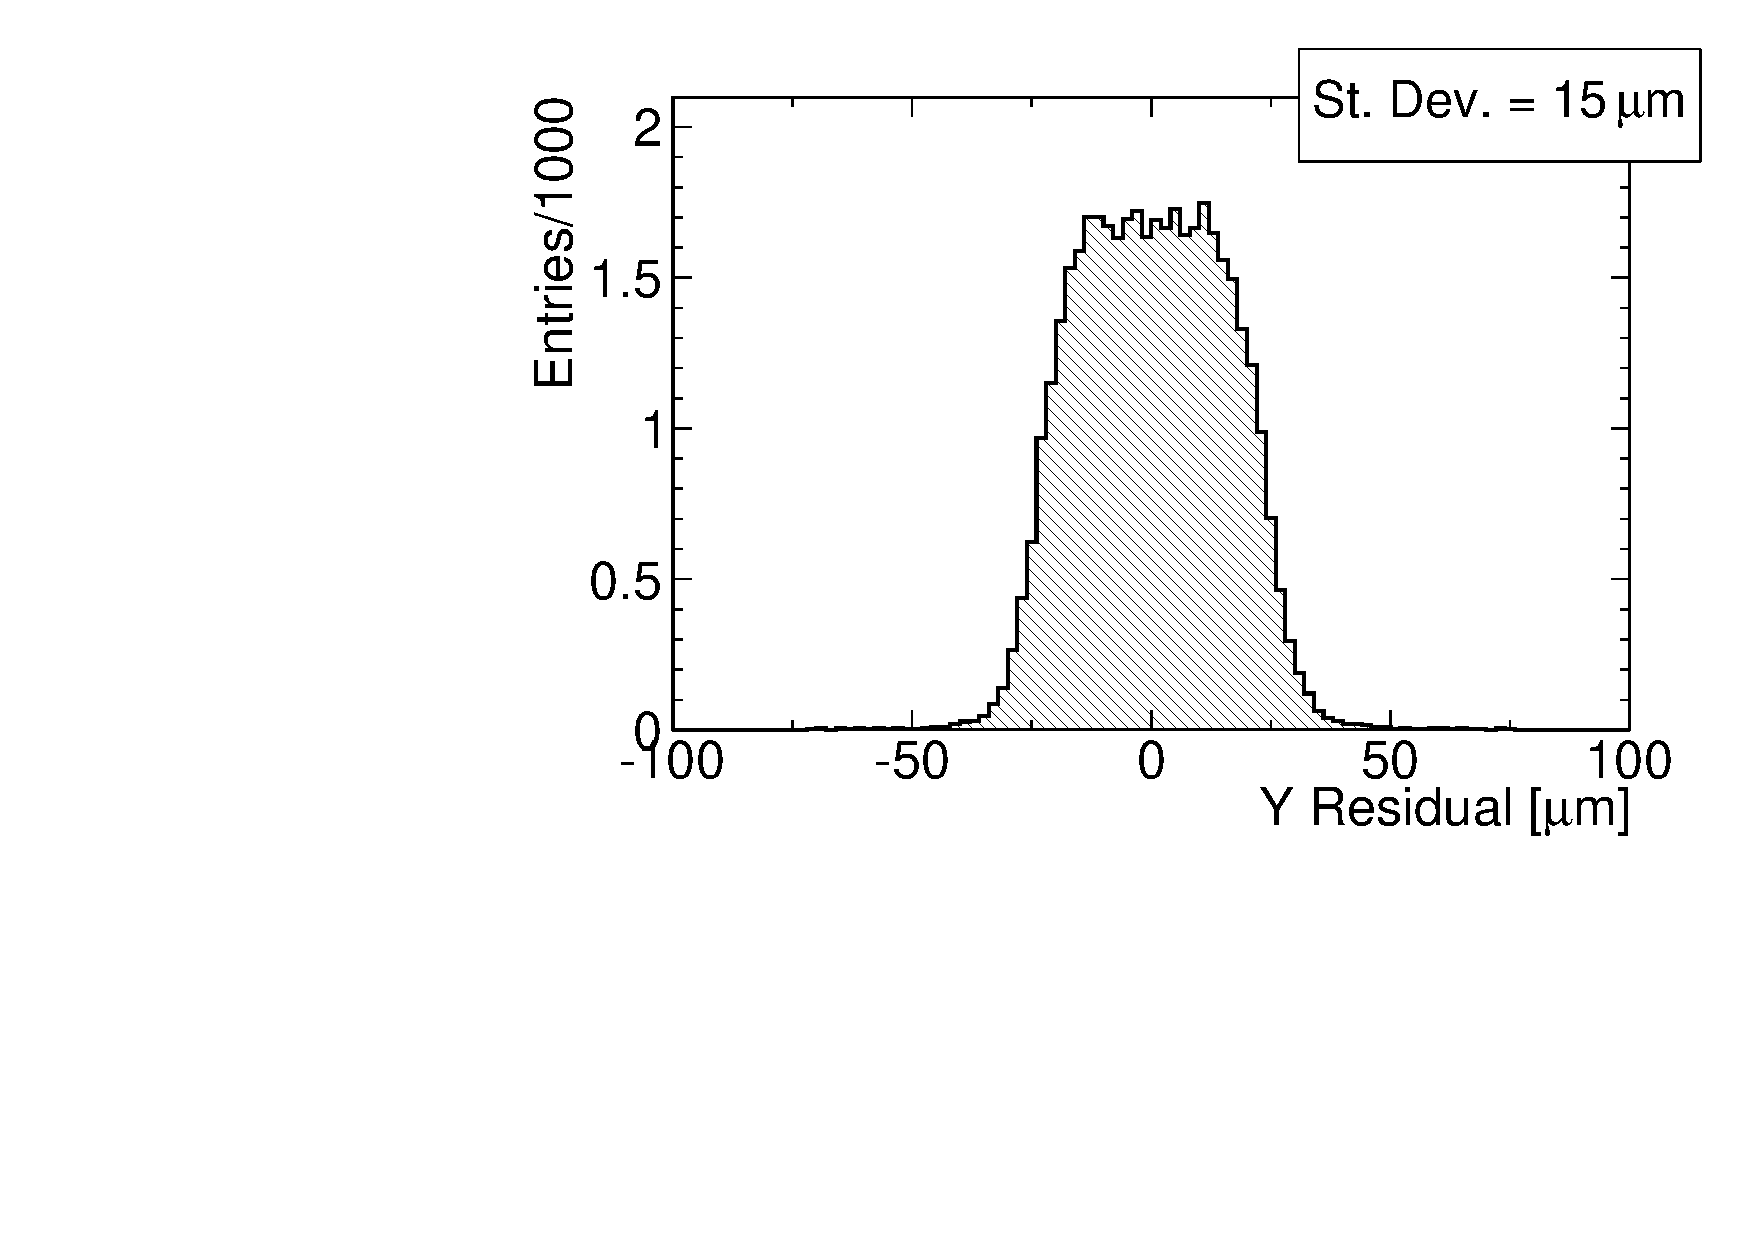
\includegraphics[width=.49\textwidth]{Oct_Period5-residuals2-11-fitResY.pdf}
 \end{center}
 \caption{Residual distributions in the short pixel direction for an unirradiated sample (DO6, left) and a sample irradiated to $2\times 10^{16}$\,n$_{\rm eq}$/cm$^2$ operated at a bias voltage of 1000\,V (DO10, right). No deterioration of the spatial distribution with irradiation is visible. \label{fig:n-in-n:residuals}}
\end{figure}


Plotting the residual distribution for two-pixel clusters only allows the width of the charge sharing region between pixels to be determined. Figure \ref{fig:n-in-n:CS2-residuals} shows the distributions for DO9 ($5\times 10^{15}$\,n$_{\rm eq}$/cm$^2$) and DO10 ($2\times 10^{16}$\,n$_{\rm eq}$/cm$^2$). After correcting for the telescope resolution, the widths of the charge sharing regions are 7.1\,$\mu$m and 7.7\,$\mu$m. These values correspond very well with the width found for an unirradiated sample of 6.4\,$\mu$m. This indicates that the lateral diffusion of the charge cloud does not change significantly with irradiation.

\begin{figure}[!hbt]
 \begin{center}
  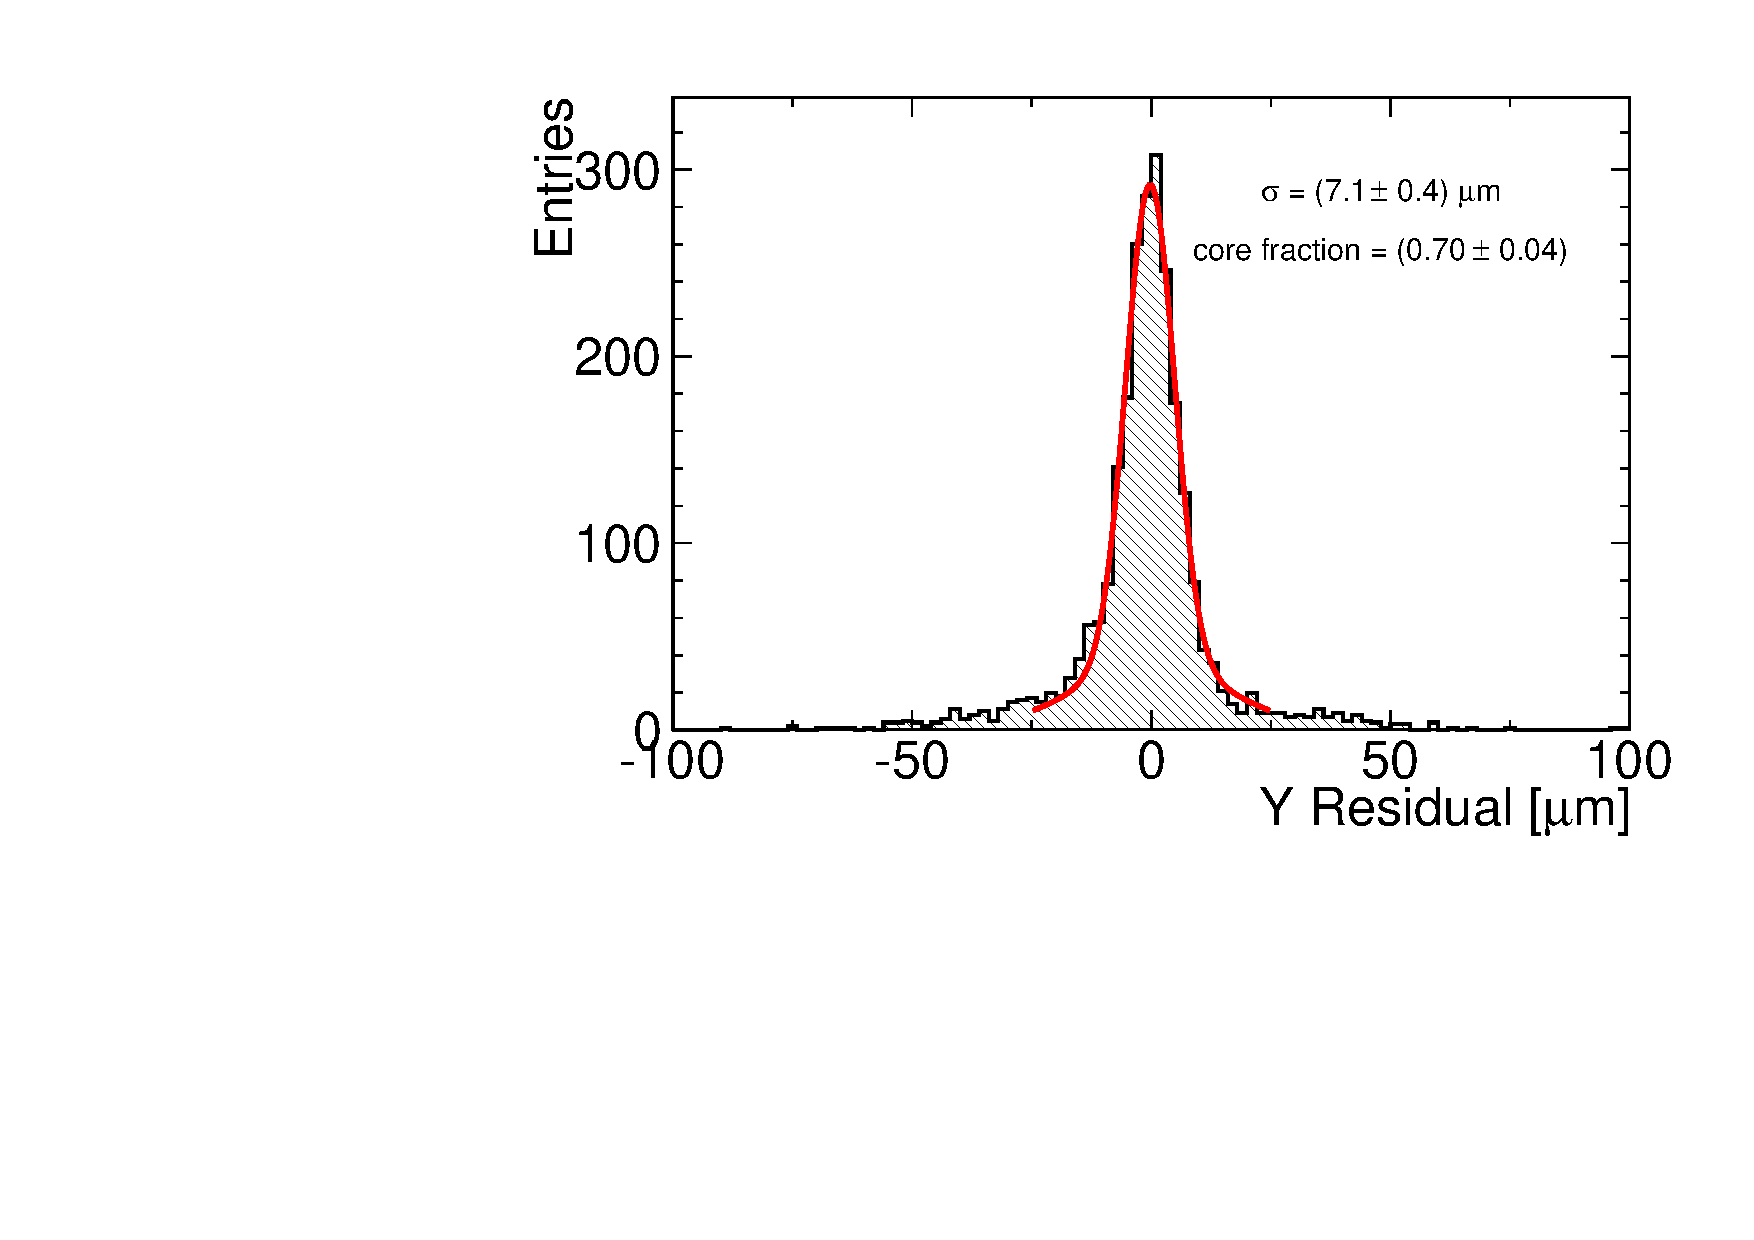
\includegraphics[width=.49\textwidth]{Oct_Period5_1-residuals2-10-cluSize2-multiG_resY.pdf}
  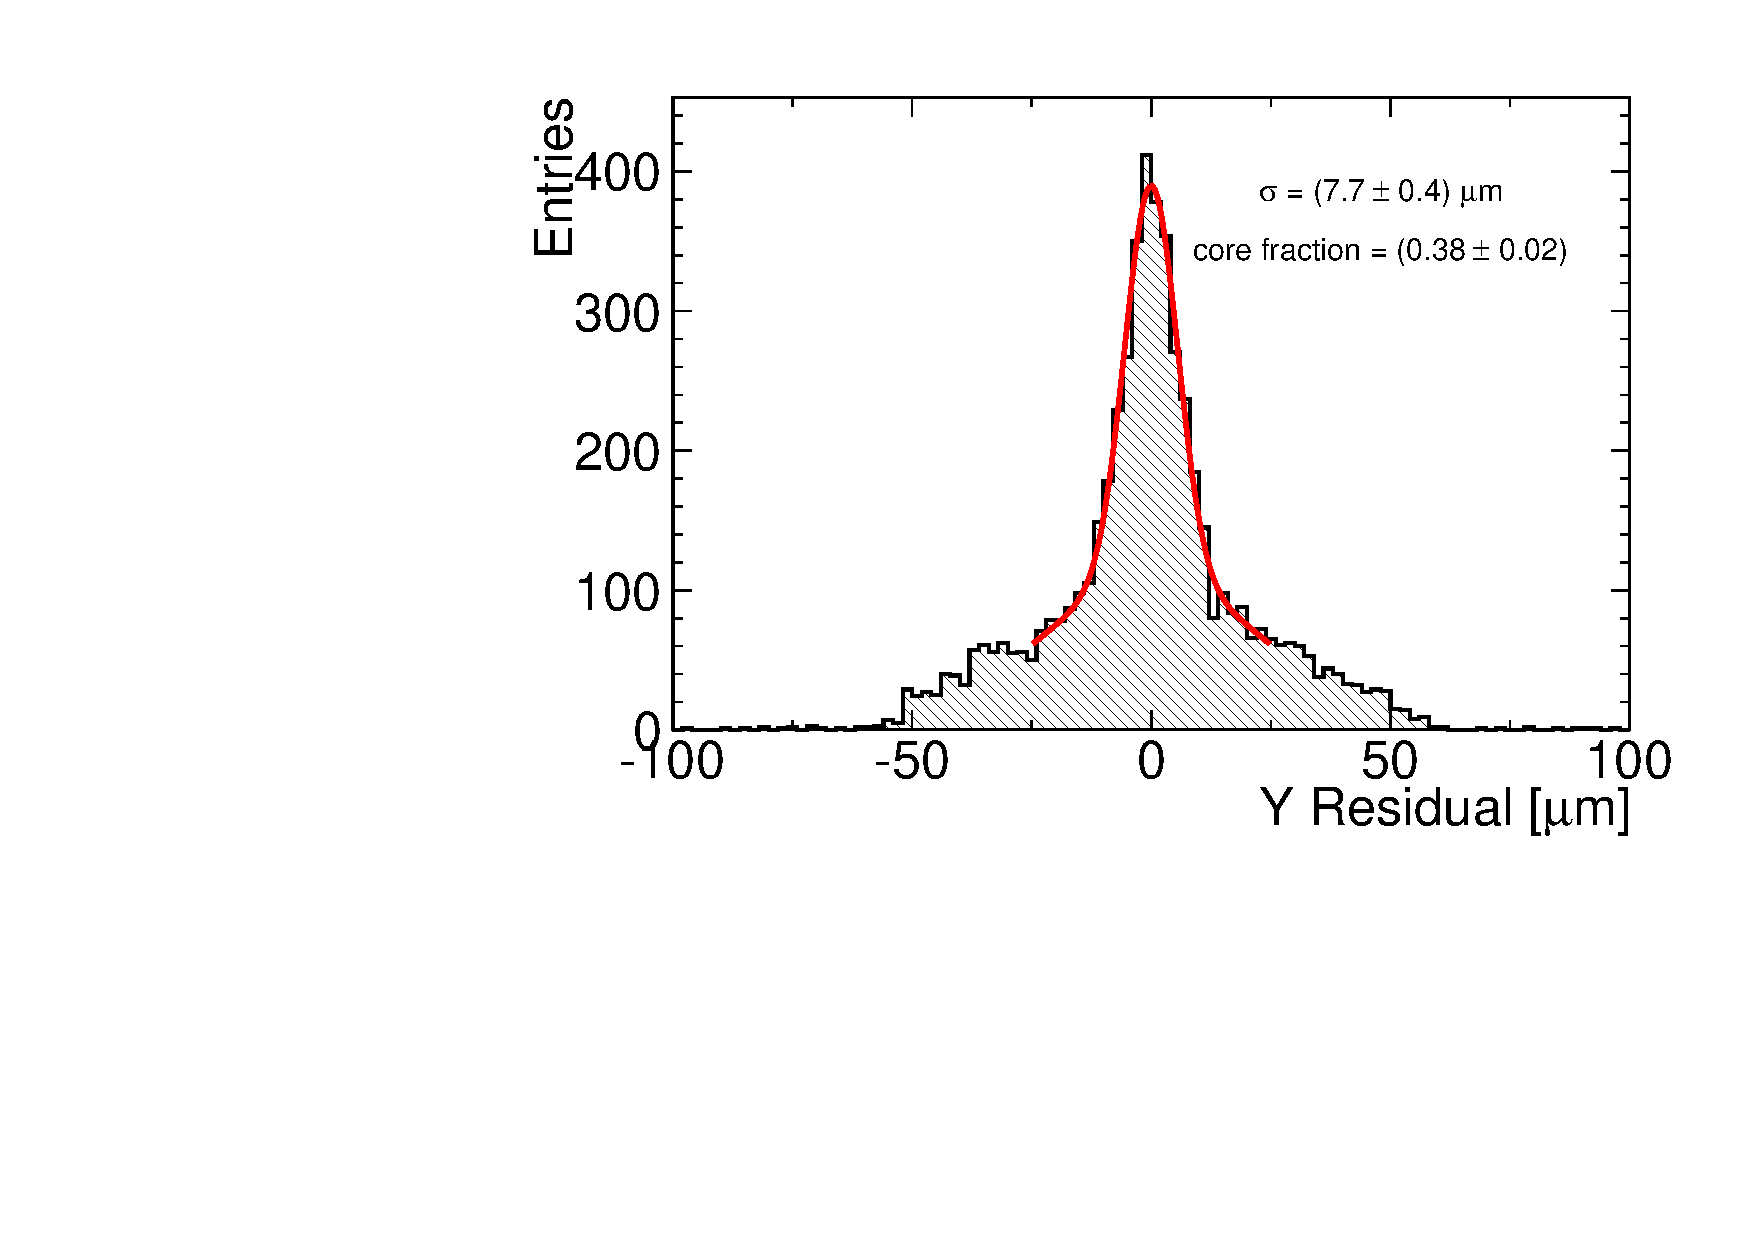
\includegraphics[width=.49\textwidth]{Oct_Period8_1-residuals2-11-cluSize2-multiG_resY.pdf}
 \end{center}
 \caption{Residual distributions for 2-pixel clusters only. Shown are distributions samples irradiated to $5\times 10^{15}$\,n$_{\rm eq}$/cm$^2$ (left: DO9, bias voltage 1000\,V) and $2\times 10^{16}$\,n$_{\rm eq}$/cm$^2$ (right, DO10, bias voltage 1200\,V), respectively. \label{fig:n-in-n:CS2-residuals}}
\end{figure}

\paragraph{Comments}
The radiation hardness of $n-$bulk sensors was tested up to unprecedented fluences, with a maximum of
 $20\times10^{15}\,{\rm n_{eq}}/{\rm cm}^{2}$.
 At a bias voltage of 1.2\,kV a collected charge of about 6\,ke was observed, corresponding to about one 
 third of the collected charge before irradiation. A much thinner detector should be able to collect a much 
 larger fraction of charge at a bias voltage lower than 1000~V.
 Despite the rather small collected charge and the reduced 
 charge sharing between pixels, no significant deterioration of the
 spatial resolution was observed. 
 Important charge losses were observed in proximity of the punch-through dot used for polarising 
 the sensor.

\subsection{Thin $n-on-p$ FE-I4 samples.}
\label{sec:PAE2pixels}

While $n-$type bulk sensors require patterned guard rings on the back side of the sensor, for $p-$type material these can be moved to the pixelated side of the sensor (front side); then metallisation is the only process for the back side. This makes it a very cost-effective material for future pixel detectors. 

Thin $n-on-p$ planar pixel sensors have been realised at FBK\footnote{FBK-CMM (Trento, Italy): \url{http://cmm.fbk.eu/}} on high resistivity type 6" 
wafers within 
the  framework of the INFN Phase-2 program~\cite{DALLABETTA2016388}.
Si-Si Direct Wafer Bonded (DWB) wafers were chosen to fabricate pixel detectors;  Si-Si DWB  are obtained bonding together two different wafers: a high-resistivity (HR) Float Zone sensor wafer and a low-resistivity (LR) Czochralski handle wafer. The FZ wafer is thinned to the desired thickness value, so as to obtain a wafer with a thin active layer plus a relatively thick mechanical support layer. P-type wafers of two different active depths (100 and 130~$\mum$) with 500~$\mum$  thick handle wafer were used. 
In Figure~\ref{fig:wafer.png} a picture of one wafer from this production.
\begin{figure}[!htpb]
\centering
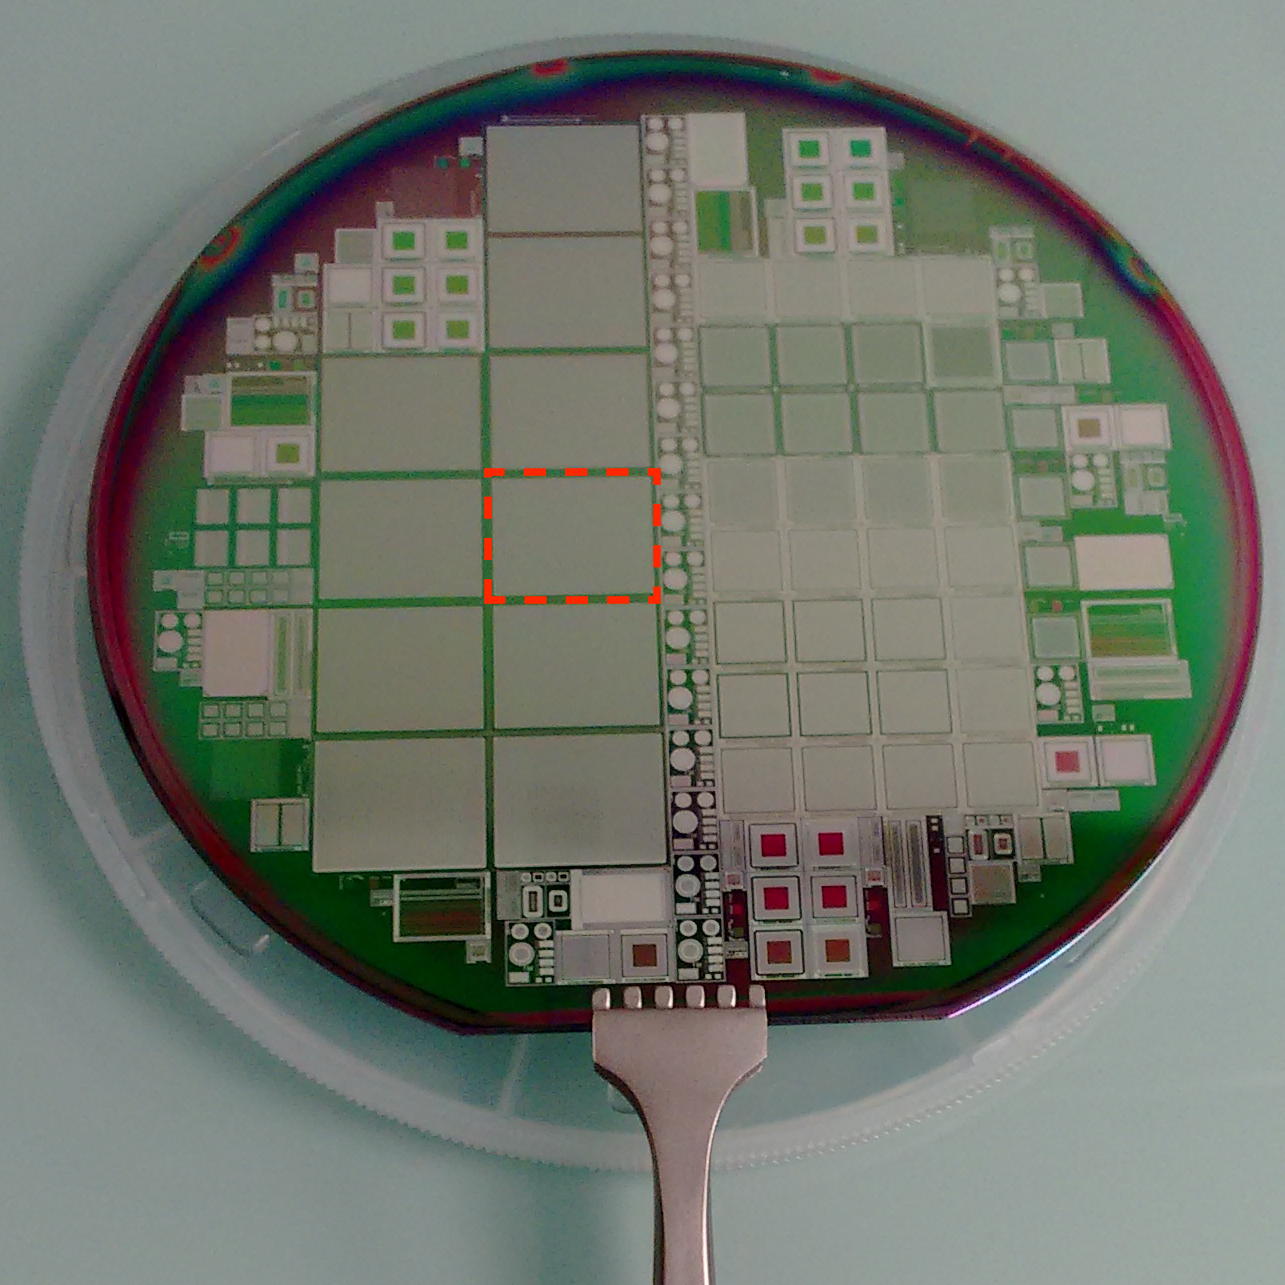
\includegraphics[width=0.35\textwidth]{wafer.png}
\caption{\label{fig:wafer.png} Wafer from the $n-on-p$ planar technology production~\cite{DALLABETTA2016388}  whose layout was mainly based on ATLAS FEI4 and CMS PSI46 designs. The red rectangle 
encircles one pixel sensors compatible with the FE-I4~\cite{FEI4} 
readout chip.}
\end{figure}

\subsubsection{Beam test studies}
Radiation hardness of that production was tested  using irradiated pixel sensors compatible with the FE-I4~\cite{FEI4} readout chip. Two sensors, {\it W80} and {\it W30}, were taken from two different sensor wafers, 
with thickness of 130 (100)~$\mum$ for W80 (W30);
and had different number of GRs,  2 and 5, respectively.  In both detector assemblies the 500~$\mum$  thick handle wafer was not thinned.

Irradiations were carried at CERN PS using the 24~GeV/c proton beam. The irradiation was staged; 
in Table~\ref{tab:W30W80Irr} the detail of the irradiation program for the two modules tested from 
that production, W80 and W30, along with their characteristics.  
\begin{table}[!htpb]
\caption{\label{tab:W30W80Irr}Irradiation program for the two FE-I4 pixel modules $W80$ and $W30$.}
\centering
\begin{tabular}{cccc}
\hline 
\hline
Module name & Beam spot size & Fluence $\phi$& Cumulative fluence at  peak $\Phi$\\ 
(thickness [$\mu$m], \# of GRs) & (FWHM - [mm$^2$]) &  [10$^{15}$ n$_\text{eq}/\text{cm}^2$]  &  [10$^{15}$ n$_\text{eq}/\text{cm}^2$] \\
\hline
W80 (130, 2) & 20$\times$20 & 3 & same\\
\hline
W30 (100, 5) & 12$\times$12 & 4 & same\\
\hline
\hline
W80 (130, 2) & 20$\times$20 & 7 & 10 \\
\hline
W30 (100, 5) & 20$\times$20 & 7 & 11\\
\hline
\end{tabular}
\end{table}

The sensors were indeed bump bonded to an FE-I4 chip at IZM, 
Berlin\footnote{Fraunhofer-Institut f\"ur Zuverl\"assigkeit und Microintegration: \url{https://www.izm.fraunhofer.de/en.html}} and measured 
on beam before and after irradiation. In Figure~\ref{fig:W80W30} some pictures of the pixel modules on 
PCB are shown. 
\begin{figure}[!htpb]
\centering
\includegraphics[width=0.36\textwidth]{scm.png}
%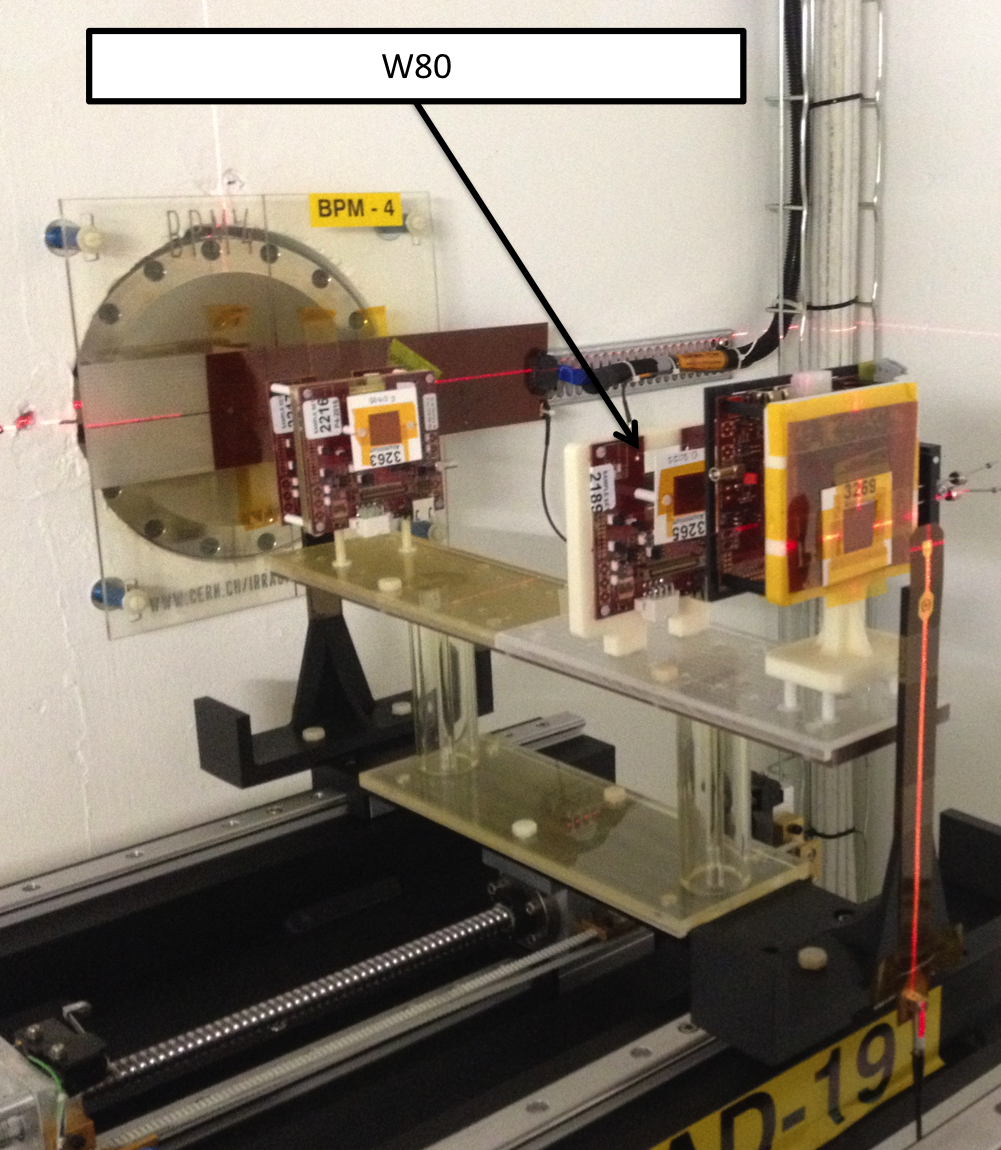
\includegraphics[width=0.25\textwidth]{w80_irrad1.png}
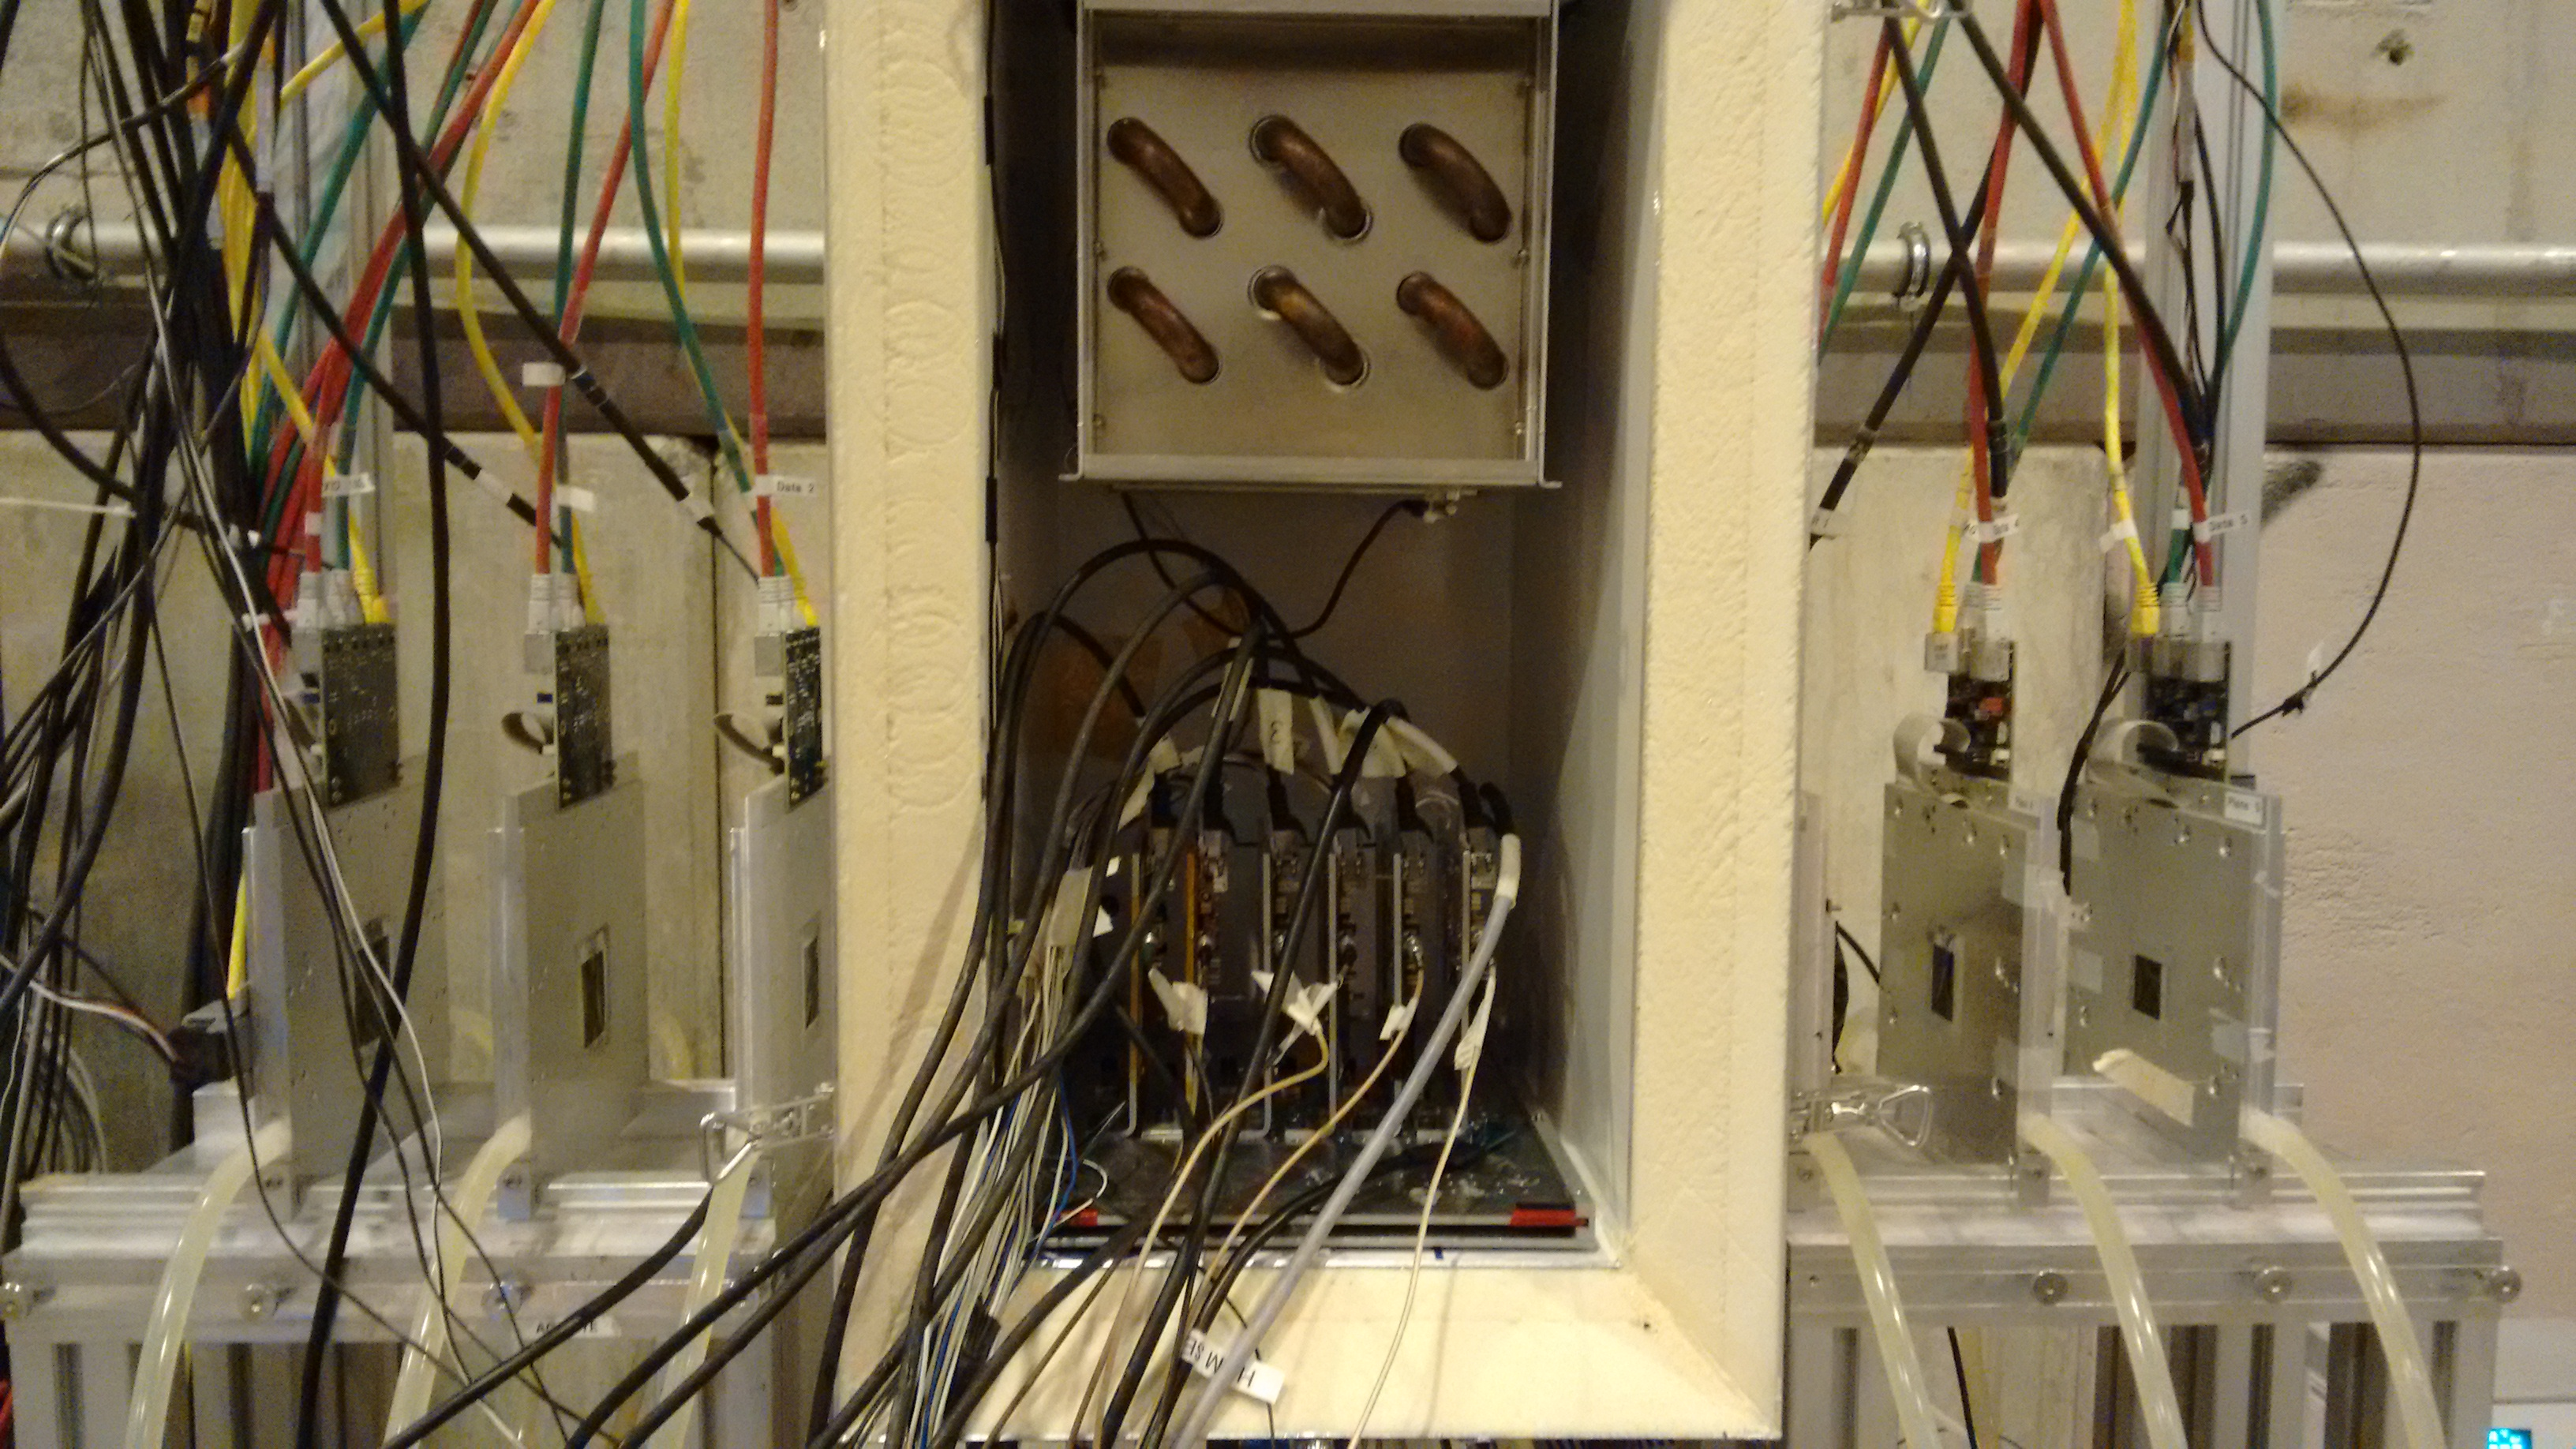
\includegraphics[width=0.63\textwidth]{in_the_box.jpeg}
\caption{\label{fig:W80W30}Thin $n-on-p$ planar pixel sensor modules. (left) Module mounted 
on a PCB card. (right) Module inside 
the DUT cooling box at the CERN H6 beamline; W80 is the second module from the left; outside 
of the box the six planes of the ACONITE telescope~\cite{Jansen2016}.}
\end{figure}

The modules were tested on beam after each irradiation step at CERN H6 beam line (120~GeV/c pions) and at DESY T21 beam line (4~GeV/c electrons).
 In both cases tracks were reconstructed thanks to  a EUDET-type beam telescope~\cite{Jansen2016}, 
 composed of six pixel detector planes equipped with fine-pitch MIMOSA 26 sensors~\cite{mimosa26}. 
 The DUTs where mounted inside a box that shed them from light and kept them cold 
 ($\sim$-35$^{\circ}$C).
 
\noindent In what follows some results are presented for hit and charge collection efficiency~\cite{TrentoWS2017,AudreyPSD11}.


\paragraph{Hit Efficiency}
Hit efficiency were tested as a function of the bias voltage for both W80 and W30 after each irradiation 
step. In Figure~\ref{fig:Hit_Eff_W80} the hit efficiency of W80 is reported after each irradiation step.



\begin{figure}[!htpb]
\centering
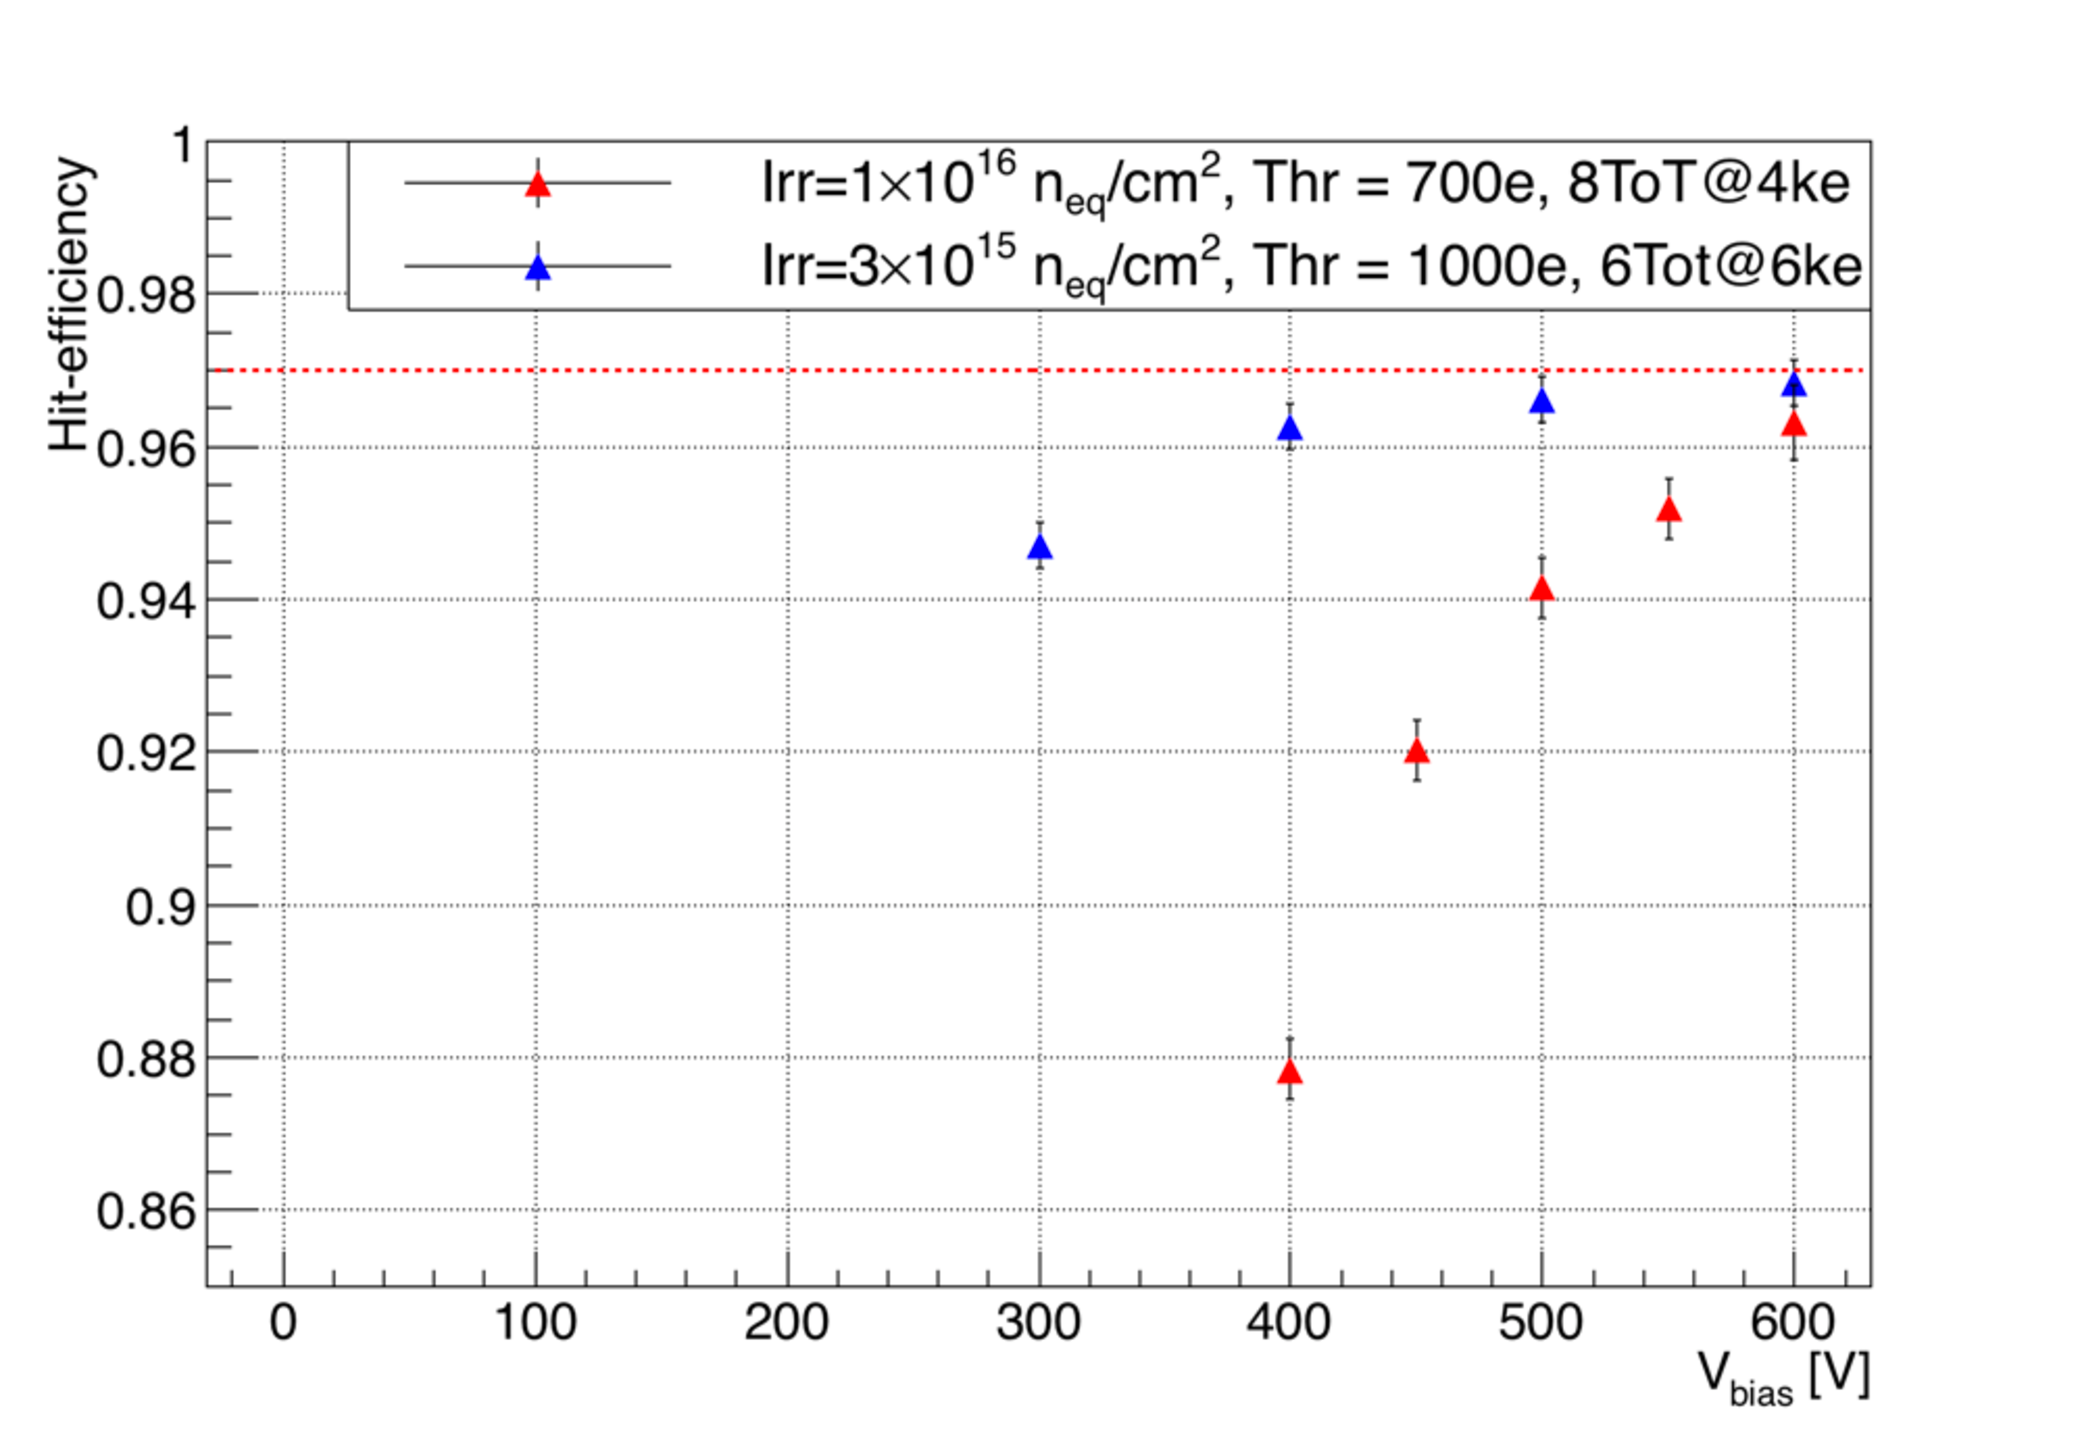
\includegraphics[width=0.65\textwidth]{new2Hit_Eff_W80.pdf}
\caption{\label{fig:Hit_Eff_W80}Hit efficiency as a function of the bias voltage for the W80 module after each irradiation step.The fluence, the threshold and the tuning 
are indicated. The red dashed line indicate the 97\% 
hit efficiency.}
\end{figure}

For the lower fluence the module hit efficiency is  97\% or more for bias voltages larger than 500~V.  This result is good 
but somewhat below the expectations as the detector is  only 130~$\mu$m thick and the fluences 
not so large (3$\times 10^{15}$ n$_\text{eq}/\text{cm}^2$). One possible explanation for this not 
so large hit efficiency is the threshold: 1000~e was probably too high for such detector. 

After a fluence of $\Phi=1\times 10^{16}$ n$_\text{eq}/\text{cm}^2$ the W80 module efficiency is close to 97\%  at a bias voltage of 600 V for a threshold of 700~e (the signal amplitude 
for a MIP in an un-irradiated module of the same thickness is about 8000~e). This result is very 
promising and it meets  the specifications for the Layer 1 of the ITk pixel detector.



The hit efficiency within the pixel cell was investigated too. In Figure~\ref{fig:NPTW80InpixelEff.pdf} 
the result for W80 after the first irradiation step. It can be seen that there are inefficient regions 
at the short sides of the pixel cell. This is consistent with the presence of permanent biasing structures 
like the $n^+$ bias dot implant and the bias rail shorting the bias dots together.

\begin{figure}[!htpb]
\centering
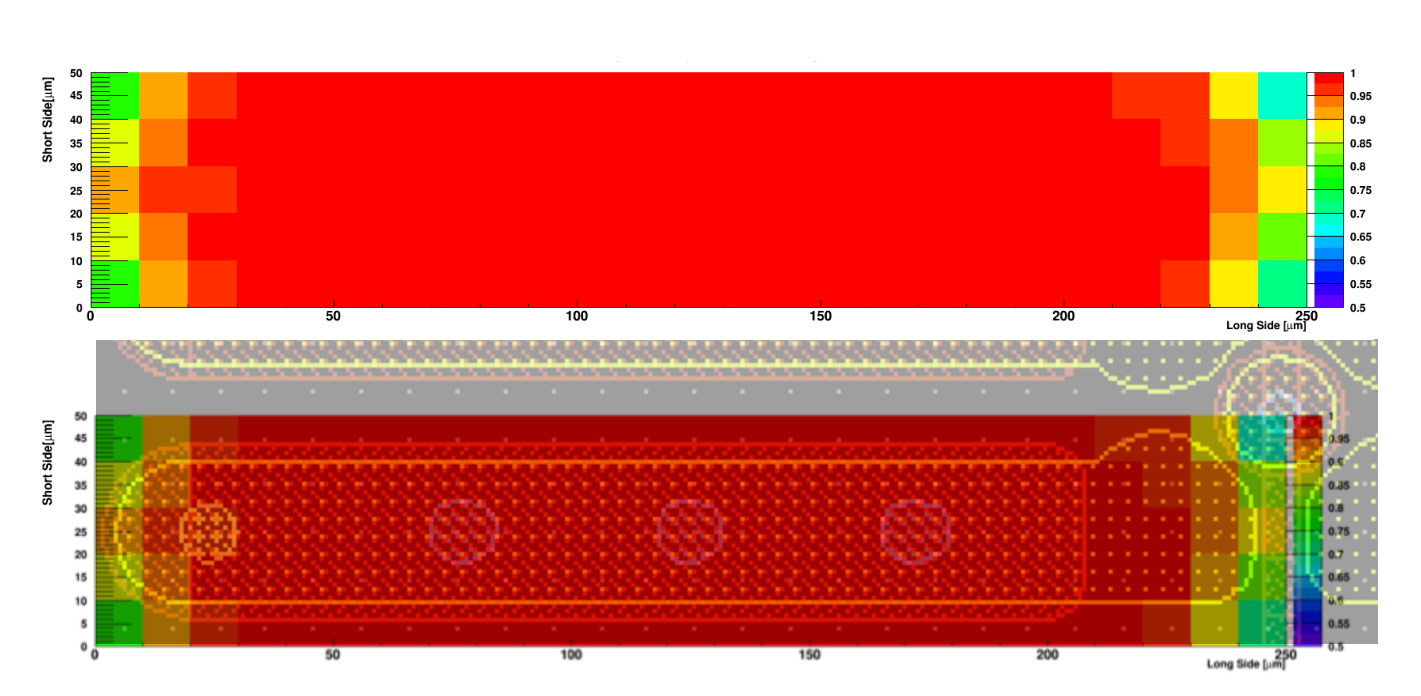
\includegraphics[width=1.00\textwidth]{NPTW80InpixelEff.pdf}
\caption{\label{fig:NPTW80InpixelEff.pdf} (top) Hit efficiency within a pixel of the W80 module after the first irradiation step. (bottom) The pixel cell layout is superimposed.}
\end{figure}

\paragraph{Charge Collection Efficiency}

The charge collection efficiency was studied for the W30 module after the  irradiation. The cluster charge distribution, measured in Time-over-Threshold bins of 25~ns~\cite{FEI4} was 
fitted with a Landau function convoluted with a Gaussian. In Figure~\ref{fig:IrrCCE} the comparison 
of the cluster charge distribution for the W30 module before and after the first irradiation step, at 100~V and 600~V 
bias voltage respectively.

\begin{figure}[!htpb]
\centering
%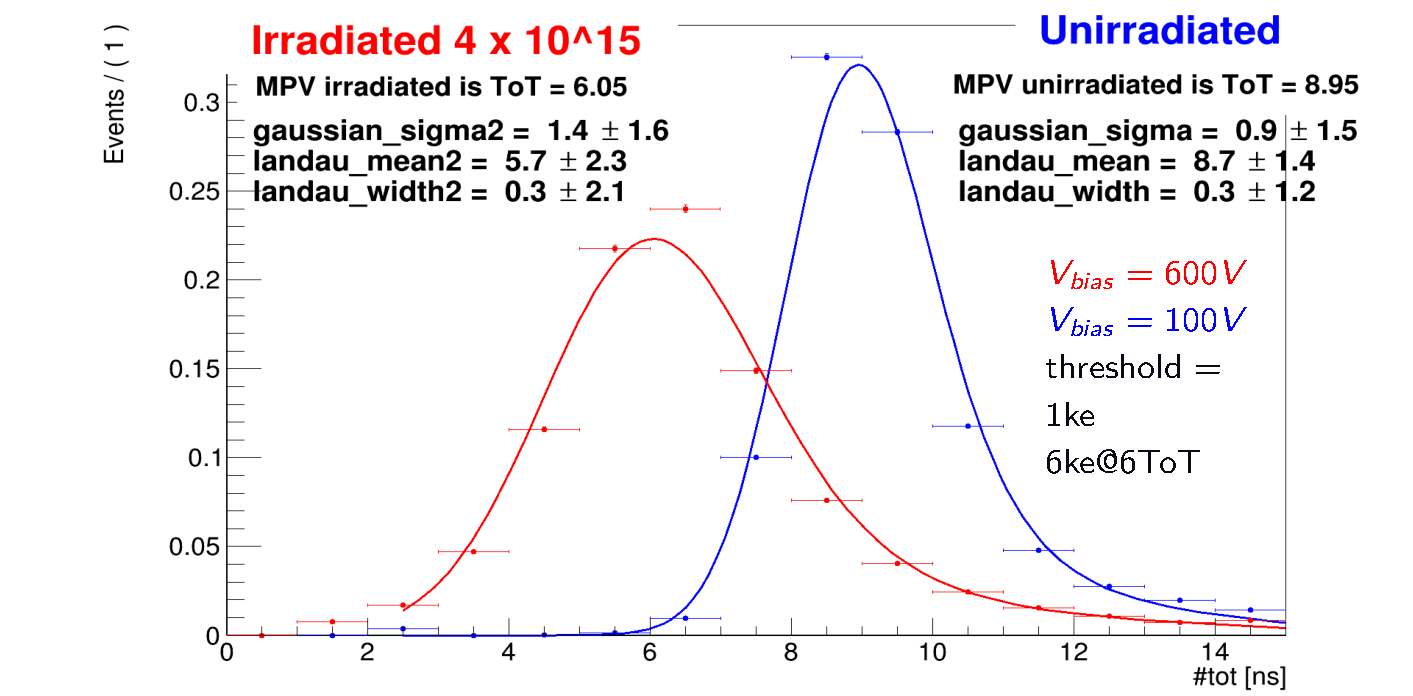
\includegraphics[width=0.75\textwidth]{IrrCCE.pdf}
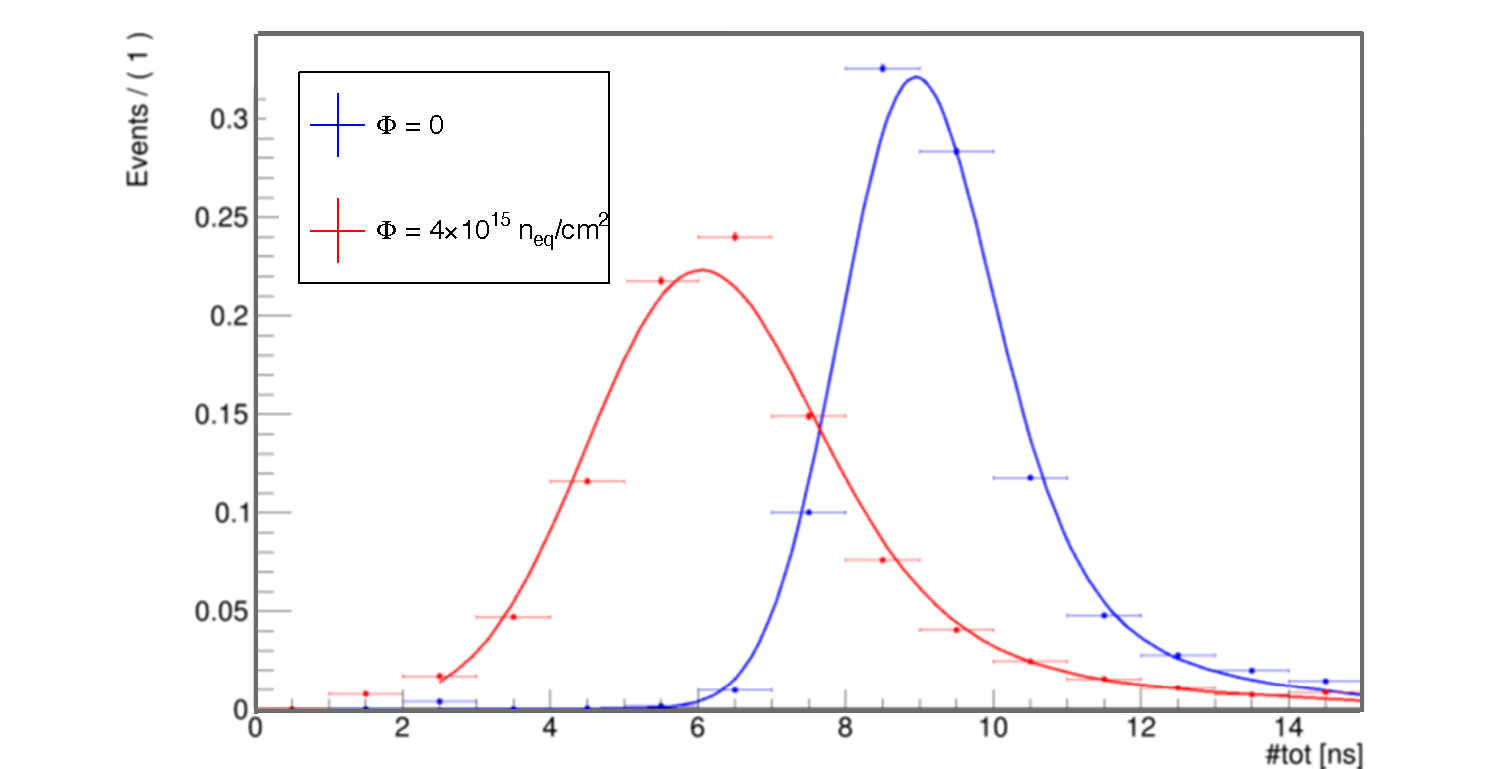
\includegraphics[width=0.75\textwidth]{CCE_4e15_W30.pdf}
\caption{\label{fig:IrrCCE}Cluster charge distribution, measured in ToT,  for the W30 module before and after the first irradiation 
step; the bias voltages were 100~V and 600~V, respectively.}
\end{figure}

Both before and after irradiation the module was tuned always with a threshold of 1000~e and 6 ToT corresponded to 6000e. 
It can be seen that after the irradiation the most probable value (MPV) of the distribution is reduced 
by about 33\%, going from 9 to 6.

In Figure~\ref{fig:new_mpv_bias} the  cluster charge distribution for the for the W80 module  after the second irradiation 
step, {\it i.e.} after a total fluence of 1$\times{16}$ n$_\text{eq}/\text{cm}^2$, at different bias voltages. 
\begin{figure}[!htpb]
\centering
%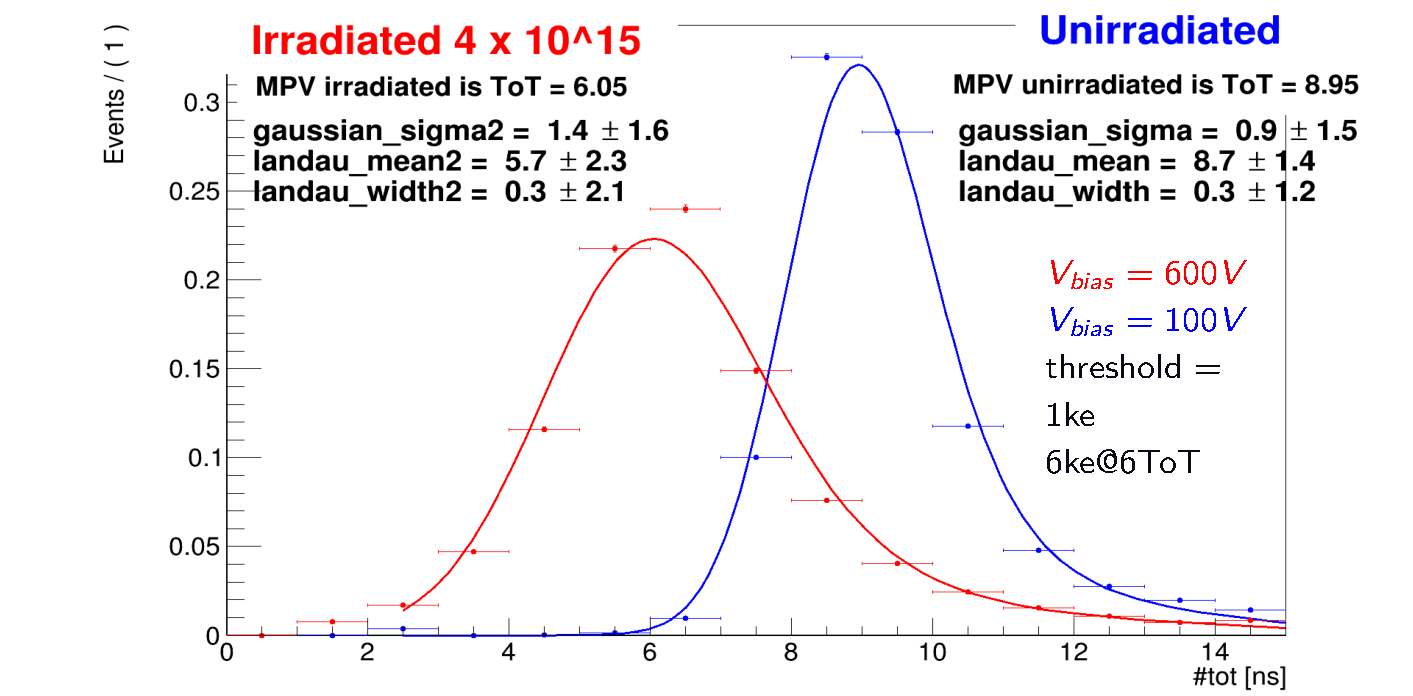
\includegraphics[width=0.75\textwidth]{IrrCCE.pdf}
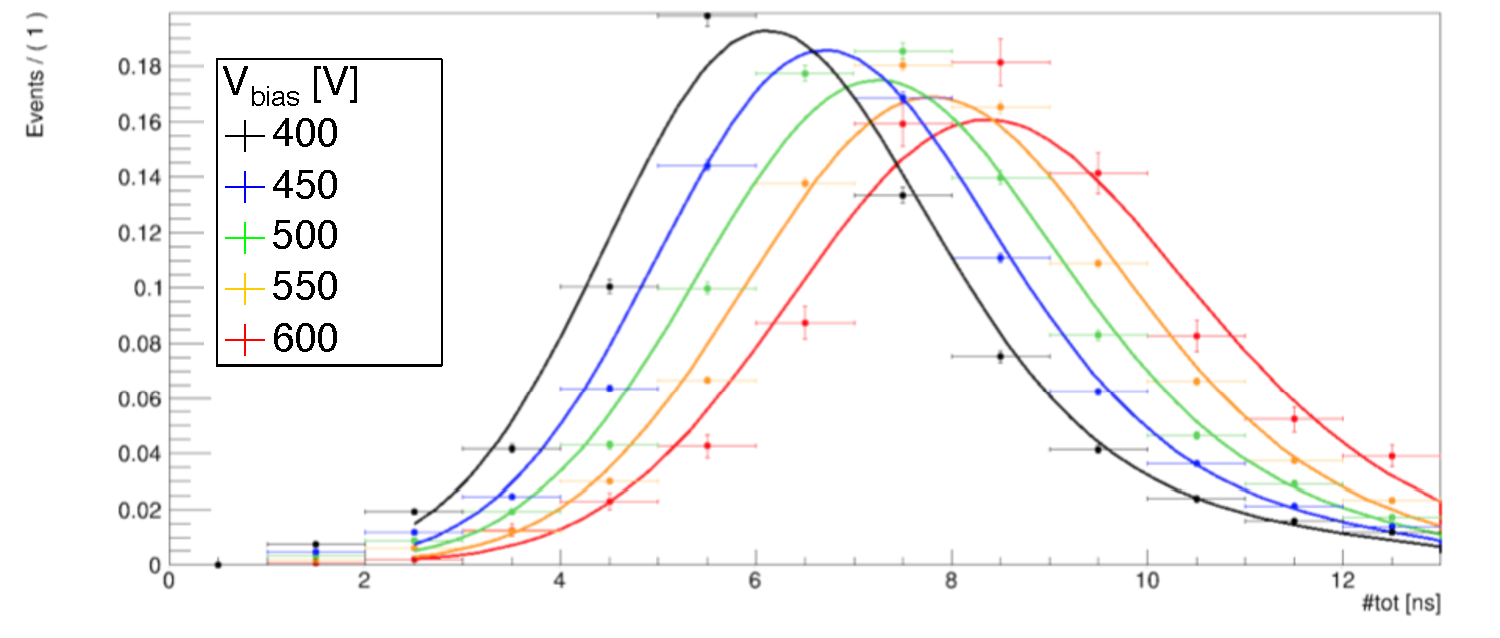
\includegraphics[width=0.75\textwidth]{new_mpv_bias.pdf}
\caption{\label{fig:new_mpv_bias}Cluster charge distribution, measured in ToT,  for the W80 module  after the second irradiation 
step.}
\end{figure}

The module was tuned always with a threshold of 700~e and 8 ToT corresponded to 4000e. 
The MPV of the cluster charge in ToT increases from $\sim$6 to $\sim$9 as the bias voltage
 changes from 400 to 600~V. 
 
 A crude estimation of the loss in the amount of collected charge 
 can be made comparing Figures~\ref{fig:IrrCCE} and~\ref{fig:new_mpv_bias}. At 600~V, after 
 a fluence of 1$\times{16}$ n$_\text{eq}/\text{cm}^2$, the 130~$\mu$m thick W80 detector 
 collects about half of the charge it was collecting before irradiation.
 
 

\paragraph{Comments}
Thin planar detectors are envisaged for the ITk pixel detector. The results reported here for 130~$\mu$m 
thick $n-on-p$ pixel modules are very promising since they exhibit an hit efficiency close to 
97\% at a bias voltage of 600~V after a fluence of 1.0$\times{16}$ n$_\text{eq}/\text{cm}^2$; 
the charge collected is half of the original one before irradiation.
 The tested 
modules were just 
prototypes that used the existing FE-I4 readout chip. New thin pixels sensors prototypes, compatible 
with the RD53A chip are in preparation; thanks to new readout chip, which should have 
the possibility to get lower in threshold, it should be possible to recover full hit efficiency even at  
bias voltages lower than 600~V. 
 

\section{Edgeless $n-on-p$ Planar Pixel Sensors}
\label{sec:edgeless}

ITk pixel sensors, other than meeting radiation hardness specifications, have to assure highest 
possible geometrical acceptance, being ``active'' almost till the physical detector edge.
In what follows edgeless sensors using the active technology will be discussed.  
In particular the results from the joint LPNHE-FBK  active edge planar pixel sensors production will be presented. They are documented in a series of documents which will be referred to.

\subsection{Edgeless Pixel Sensors and the Active Edge Technology}

As for the IBL (see Section~\ref{sec:IBLoverview}) for the ITk pixel barrel layers too there will be no 
space for module tiling in the $z$ (beam) direction. So the fractions of inactive regions have to be kept 
low by having larger pixels at the edge and in the regions between chips, and by minimising the edge 
region while still preventing voltage breakdown. 
 The ITk specifications indicate that the distance from the active region to the cut edge of pixel modules has to be smaller than 100~$\mu$m~\cite{ITkStripsTDR} in all pixel layers and rings.



The 3D sensor technology inherently allows for slim edges of 15-150~$\mu$m~\cite{1748-0221-10-03-C03031} 
Planar sensors can adopt slim edge designs, as it was done for the IBL pixels sensors, or 
an edgeless design, through the ``active edge'' technology.


The active edge is one of the possible choices to realize ``edgeless'' detectors, {\it i.e.} detectors with no (or very limited) insensitive area. Along the sensor border a trench is dug by deep reactive ion etch (DRIE), reaching through the whole thickness of the substrate (hence a support wafer is required).  The  trench is then doped with boron (for $p-$type bulks) and  filled with polysilicon. The cut realized through DRIE produces an edge region
much less damaged than the one resulting from a standard diamond-saw cut. This leads to less generation centers hence lower leakage current generated at the border. Moreover, the edge doping prevents the depletion region from reaching the physical trench walls, hence carriers created at the edge  do not experience an electric field, are not effectively separated and just recombine, without contributing significantly to the device leakage current.
Active edge technology can routinely obtain very uniform, well defined and narrow trenches, as shown for example in Figure~\ref{fig:trench}. For a 200~${\rm \mu}$m thick bulk the typical trench width is of~5~${\rm \mu}$m.

\begin{figure}[!htpb]
\begin{center}
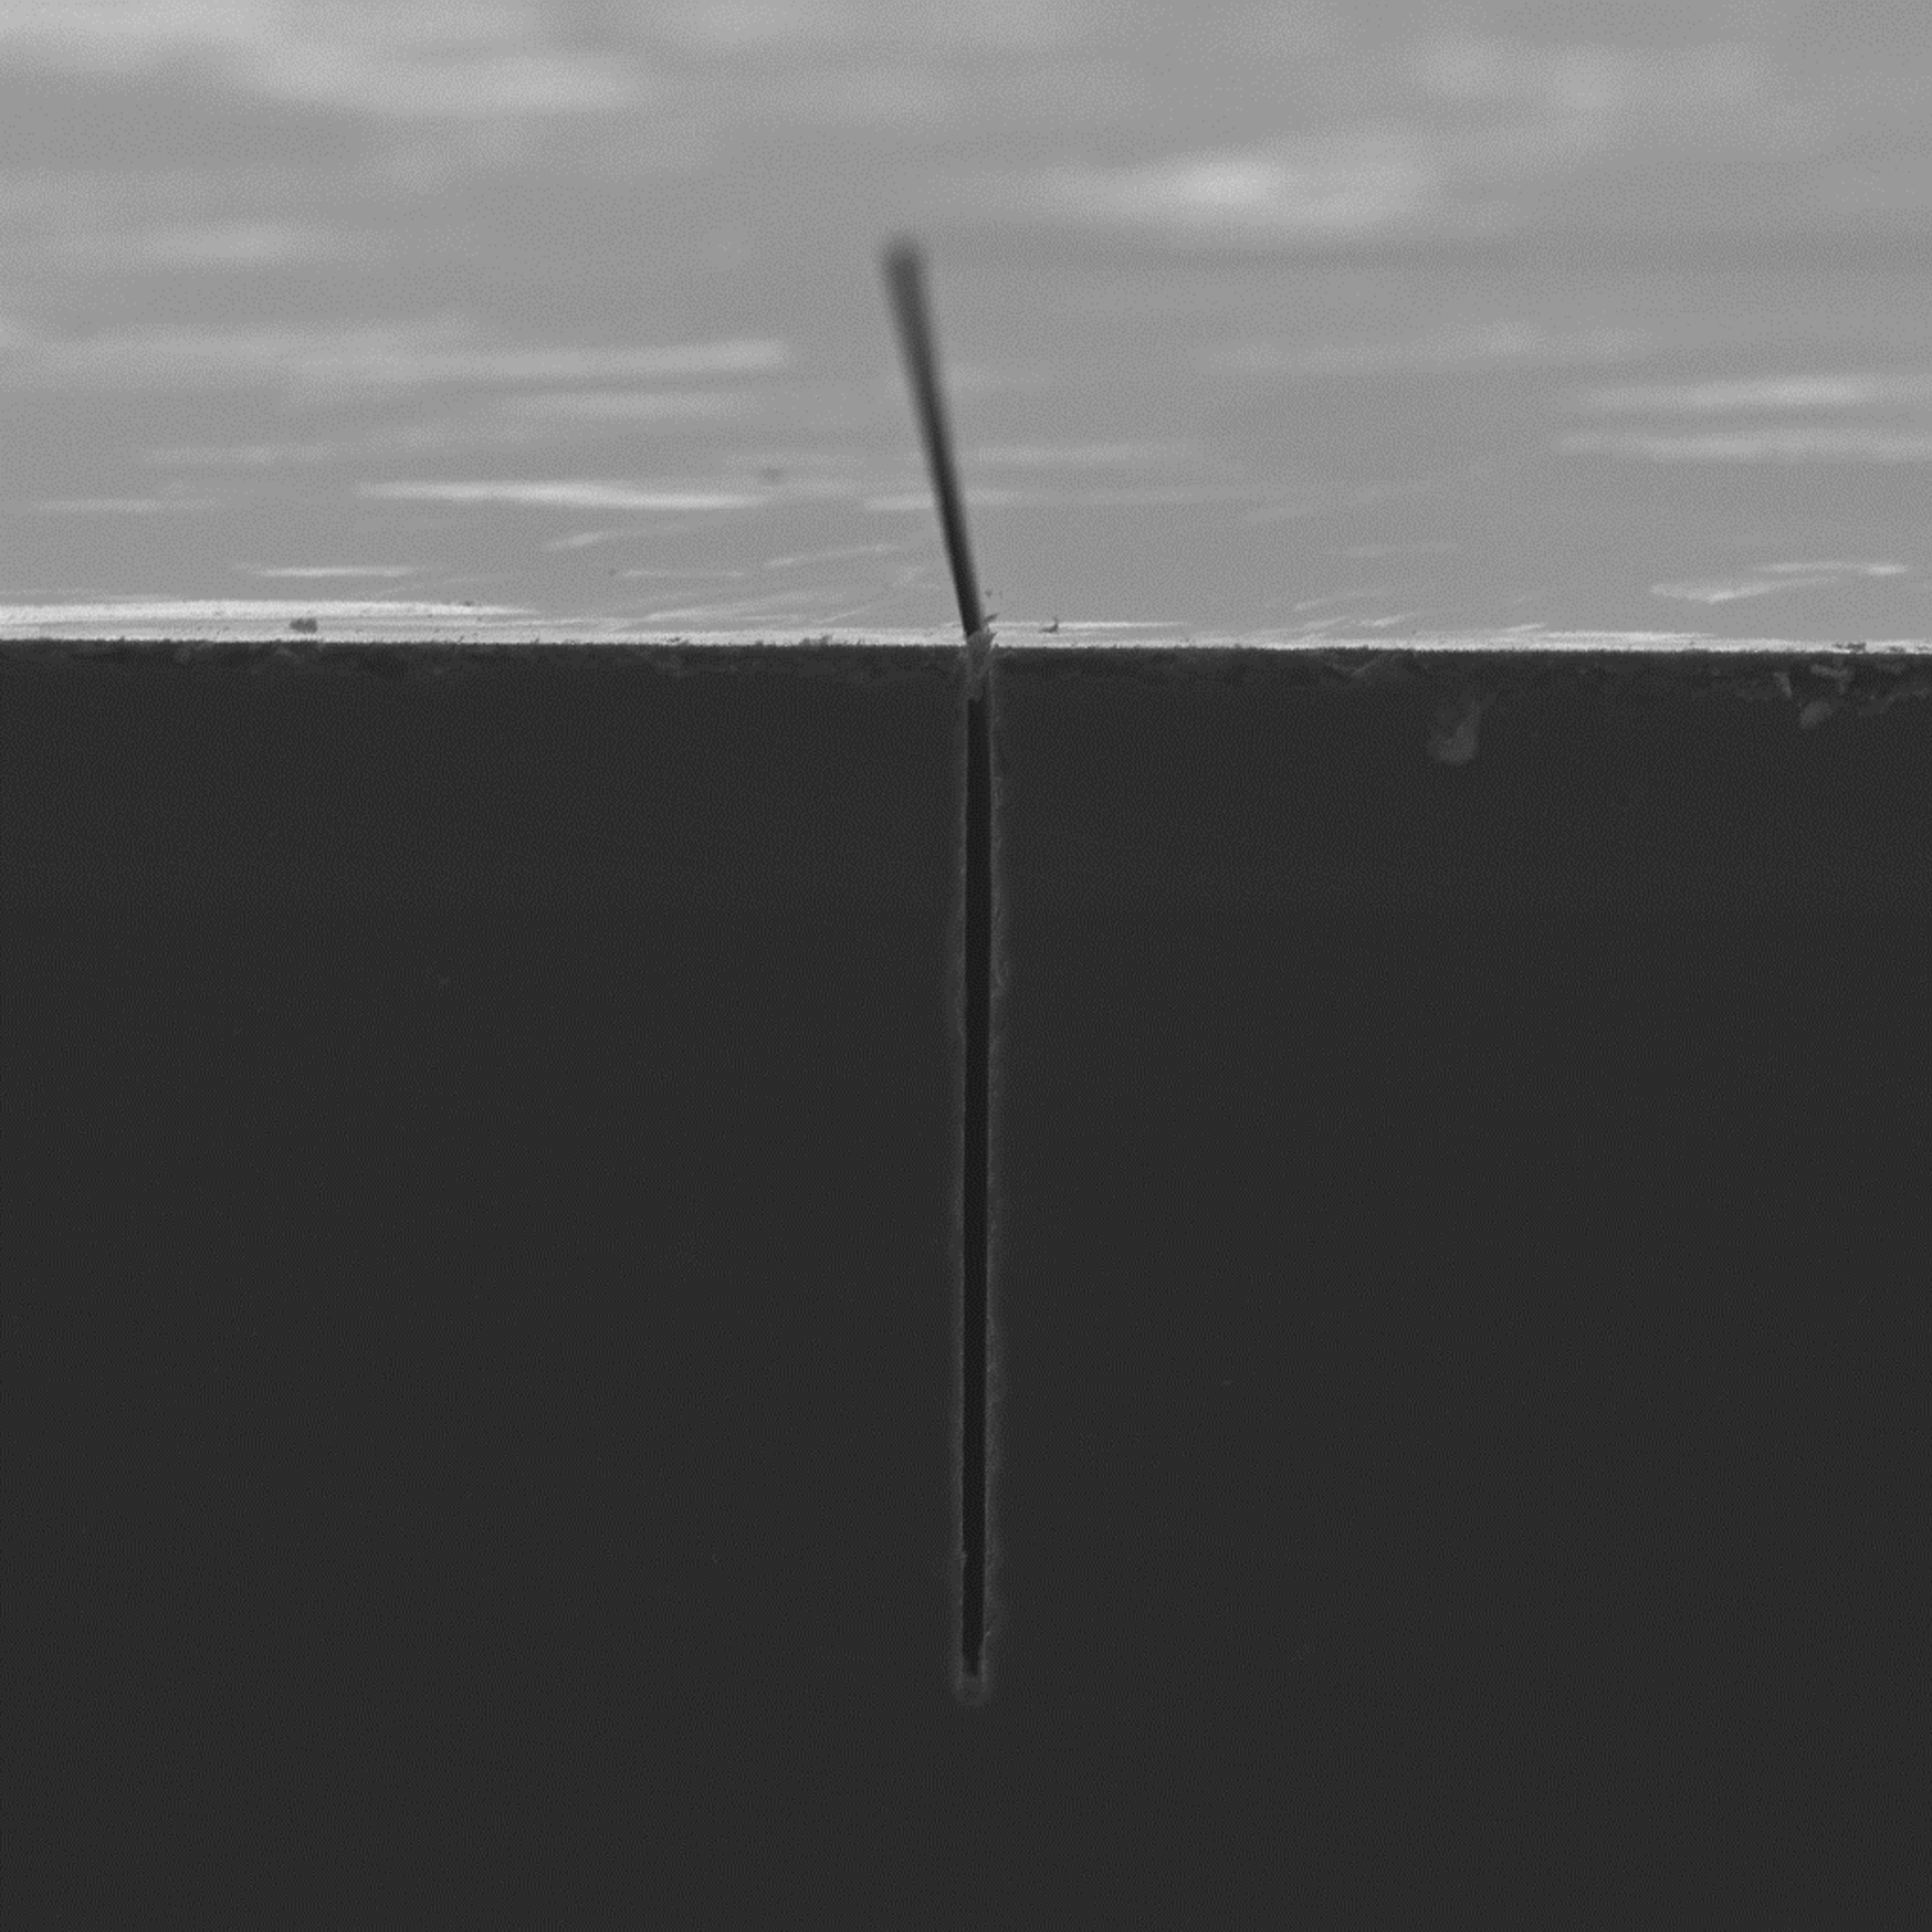
\includegraphics[width=0.40\textwidth]{trench.pdf}
\caption{\label{fig:trench}SEM picture of  a test trench, after cleaving the wafer perpendicularly to the surface and to the trench itself.(After~\cite{bib:nim2012})}
\end{center}
\end{figure}


\subsection{Joint LPNHE-FBK  Active Edge Planar Pixel Sensors Production}
The active edge technology was chosen  by LPNHE~\footnote{Laboratoire de Physique Nucleaire et de Hautes \'Energies (LPNHE), Paris, France; \url{http://lpnhe.in2p3.fr/}} for a  planar pixel production
 with reduced inactive zone~\cite{bib:nim2012}.
The production, composed of 200~$\mu$m thick $n-on-p$ sensors, was realised at FBK\footnote{FBK-CMM (Trento, Italy): \url{http://cmm.fbk.eu/}}.

\subsubsection{The Active Edge Sensor Fabrication at FBK}
Since the trench extends all the way through the sensor wafer thickness, the support wafer has to 
be bonded to the sensor one before starting the etching step.
Given the presence of the  support wafer  accessing the backside  after wafer-bonding is impossible.
Thus, as first process steps, a uniform high-dose boron implant has been performed on the back side, 
followed by a thermal oxide growth on
both sides.

Up to the trench definition, the process follows standard steps. Since the read-out electrodes are n-type, they will be shorted together by the electron
inversion layer, induced by the positive fixed charge present in the oxide, unless a p-type implant, compensating such charge, surrounds the pixels.
Both homogeneous (``p-spray'') and patterned (``p-stop'') implants have been used;
the process splittings adopted in the fabrication batch only concern the presence and the doses of these implants,  as detailed in table~\ref{tab:isolation}.



\begin{table}[!htpb]
\caption{\label{tab:isolation}List of the different isolation solutions adopted in the process.}
\begin{center}
\begin{tabular}{cc}
\hline
p-spray    & p-stop \\
\hline
\hline
  low dose &      absent\\
  high   dose  &   absent\\
  low   dose &     present\\
  high  dose  &   present\\
  absent  &   present
\end{tabular}
\end{center}
\end{table}

Two patterned high dose implants, a  phosphorus implant forming the pixel and GR junctions  and a boron implant for  the ohmic contact
 to the substrate (``bias tab''), are then performed.

The etching of the trench is accomplished by a Deep Reactive Ion Etching (DRIE) machine, the same used for the fabrication of
3D detectors~\cite{bib:3DFBK}. The trenches in an active edge sensor must be fully passing, {\it i.e.} their bottom  has to reach  the silicon oxide, which separates the active wafer from the 
support wafer.

After the trench is etched, its walls are boron-doped in a diffusion furnace.
Thus, a continuous ohmic contact to the substrate  is created on the trench wall and to the backside.

The trenches are then oxidized and filled with polysilicon.
The remaining processing, arriving at the final device, whose cross-section is sketched in Figure~\ref{fig:pixel},
is quite standard, and includes the following steps:
\begin{itemize}
\item contact opening
\item metal deposition and patterning
\item deposition of a passivation layer  (PECVD  oxide)  and patterning of the same in the
 pad and bump-bonding regions.
\end{itemize}

\begin{figure}[!htpb]
\begin{center}
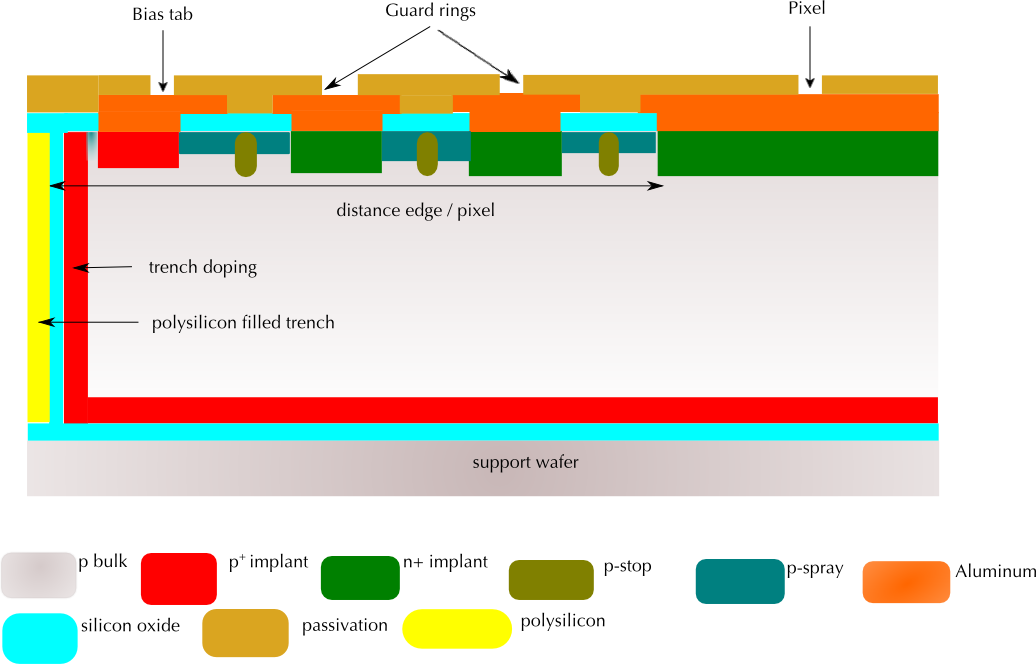
\includegraphics[width=0.65\textwidth]{pixel_design_v3.png}
\caption{\label{fig:pixel}Schematic section of the pixel sensor. The region close to the sensor's edge is portrayed, including the pixel closest to the edge,
the edge region, including GRs (when present), the bias tab (present only on one edge of the device), the vertical doped trench, and the support wafer.}
\end{center}
\end{figure}

Since some sensors were intended to  be bump-bonded to  FE-I4~\cite{FEI4} read-out chips, 
it was necessary to select good sensors at the wafer level, by measuring their I-V characteristics.
 For this purpose, an additional layer of metal was deposited over the passivation and patterned into stripes, each of them shorting together a row of pixels, contacted through
 the small passivation openings foreseen for the bump bonding.
This so-called {\it temporary metal} solution has already been adopted for the selection of good 3D FE-I4 sensors for the ATLAS IBL~\cite{bib:metal}.
After the automatic current-voltage  measurement
 on each FE-I4 sensor, the metal was removed by  wet etching, which does not affect the electrical characteristics  of the devices.
Pictures of FE-I4 sensor pixels before and after the metal layer removal can be seen in Figure~\ref{fig:tempmetal}.

\begin{figure}[!htpb]
\centering
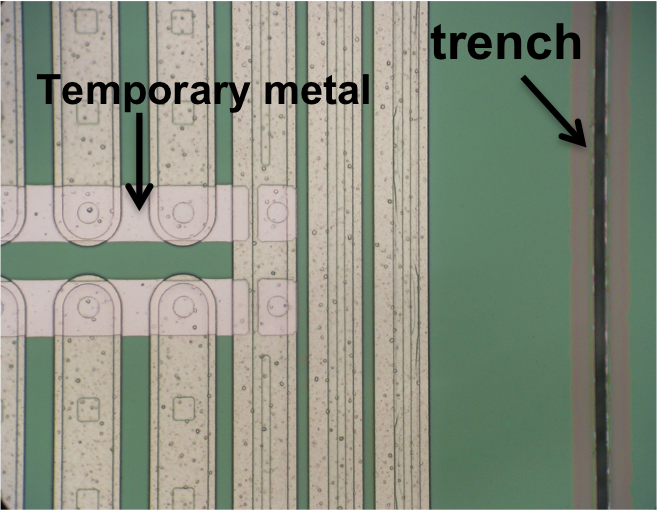
\includegraphics[width=0.49\textwidth]{annotated_temporarymetal.png}
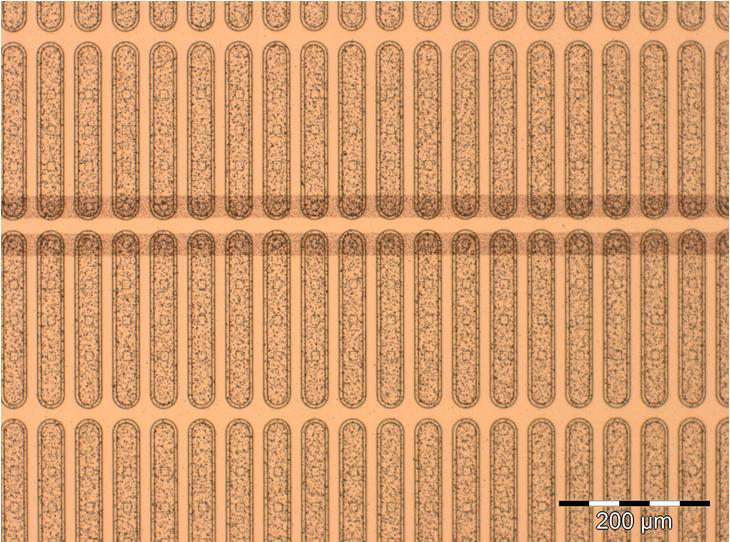
\includegraphics[width=0.49\textwidth]{notemporarymetal-izm.png}
% where an .eps filename suffix will be assumed under latex, 
% and a .pdf suffix will be assumed for pdflatex; or what has been declared
% via \DeclareGraphicsExtensions.
\caption{Pictures of the pixels-side of a FE-I4 sensor. (left) Sensors before temporary metal removal; region covered with temporary metal and the trench are highlighted. (right)
Same sensor as above (different scale, though)  after temporary metal removal.}
\label{fig:tempmetal}
\end{figure}

To further proceed in module construction  the support wafer has to be removed. The approach followed is illustrated in Figure~\ref{fig:lapping}~\cite{Bomben:2013vua}. Each FE-I4 sensor is
surrounded by the trench on all sides, so  the sensor is effectively isolated  on all sides from the silicon wafer.
After having deposited a dicing tape on the pixel side, the support wafer can be back-lapped completely. Since the trench penetrates  the whole sensor wafer thickness,
once the support wafer has been completely lapped, each sensor can separated from the others by removing the tape.


\begin{figure}[!htpb]
\centering
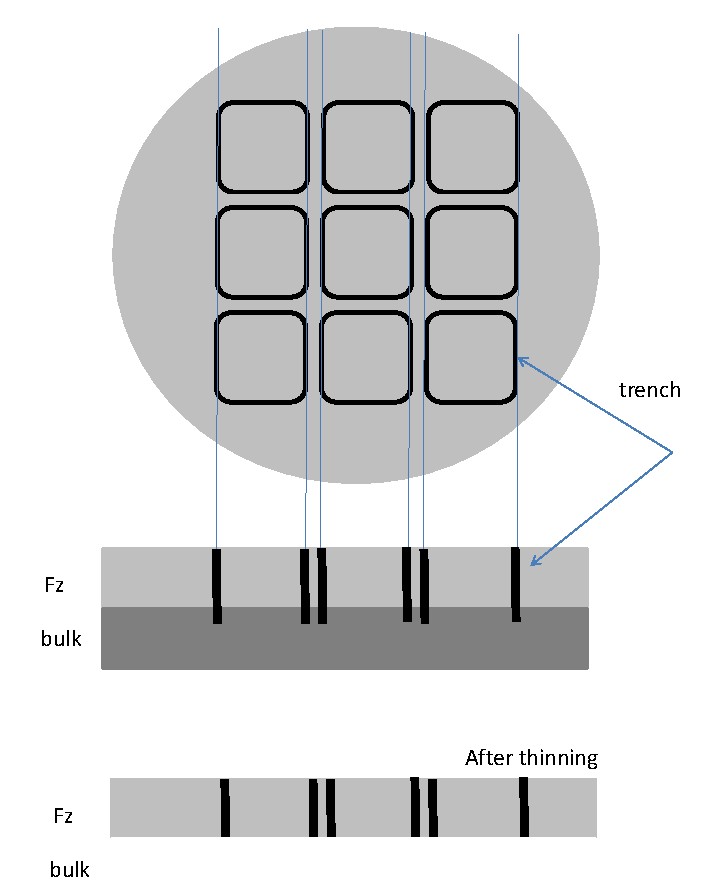
\includegraphics[width=0.55\textwidth]{edgelesslapping.pdf}
\caption{Sensors separation from wafer.}
\label{fig:lapping}
\end{figure}


After the temporary metal and the support wafer removed, the diced sensors were ready to be 
bump-bonded to the FE-I4 readout chip.


\subsubsection{The Wafer Layout}
The production included nine FE-I4 compatible pixel sensors, differing in the pixel-to-trench distance (100, 200, 300, and 400~${\rm \mu}$m) and in the number of the guard rings (0, 1, 2, 3, 5, and 10)
surrounding the pixel area (see Figure~\ref{fig:pixel}). As a reminder the ATLAS pixels feature 
100~$\mu$m pixel-to-edge distance; IBL ones 250~$\mu$m.

The sensor with 3 GRs and a 200~$\mu$m pixel-to-trench distance featured two different GR designs, and
each of them is repeated twice.
A list of the different FE-I4 sensor versions is reported in Table~\ref{tab:layout_split}.


\begin{table}[!htpb]
\caption{\label{tab:layout_split}List of FEI4 sensors.  The number of the sensors (first column) is reported for each combination of number of GRs and pixel-to-trench distance.
Two different designs are envisaged for the sensor with 3 GRs and 200~$\mu$m pixel-to-trench distance. See text for more details.}
\begin{center}
\begin{tabular}{ccc}
\hline
Multiplicity & Number of GRs & \begin{tabular}[x]{@{}c@{}}pixel-to-trench\\ distance (${\rm \mu m}$)\end{tabular}   \\
\hline
\hline
1 & 0 & 100 \\
1 & 1 & 100 \\
1 & 2 &100 \\
%3 & 200 \footnote{2 different designs} \\ 
4 & 3 & 200 \\
1 & 5 & 300 \\
1 & 10 & 400
\end{tabular}
\end{center}
\end{table}

A bias tab for substrate biasing (either by probing or by wire bonding),
 located internally to the surface delimited by the trench, was placed at about 1.5~mm from the pixelated area on
one of the sides (see also Figure~\ref{fig:pixel}).

The production included FE-I3~\cite{FEI3} compatible pixels, baby strips detectors and a  large number of test structures, {\it i.e.} square diodes and small arrays of FE-I4-like pixels, which differ in the number of
GRs surrounding the active area and in the trench-to-pixel distance.  Several possible combinations  
have been implemented, including all  those used for the FE-I4 sensors.
The aim of these structures was to  test the isolation and to measure the high-voltage behavior before 
and (possibly) after irradiation, in order to find the best sensor configuration
 to be
bump-bonded to the read-out chip and to select the best combination of GR number and trench distance 
for  possible future productions.

\subsection{Electrical Characterization}
Only one out of 20 processed wafers was not usable due to bad wafer-bonding. The electrical characterization of the production for non-irradiated sensors was been performed~\cite{Bomben:2013cia}.
It started with measurements on specially designed test structures, to assess mainly bulk and surface 
properties, then tests on large sensors followed.
The first part of the measurement program was carried mainly on structures reported in Figure~\ref{fig:pix_cap_struct}.

 \begin{figure}[!htbp]
\begin{center}
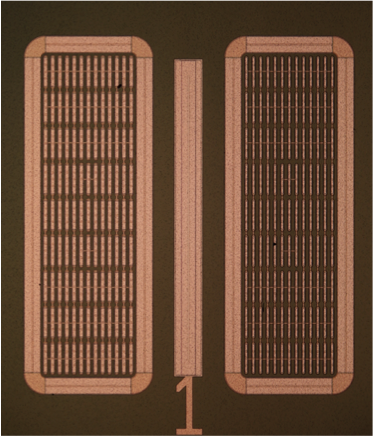
\includegraphics[width=0.29\textwidth]{pixel_cap_struct.png}
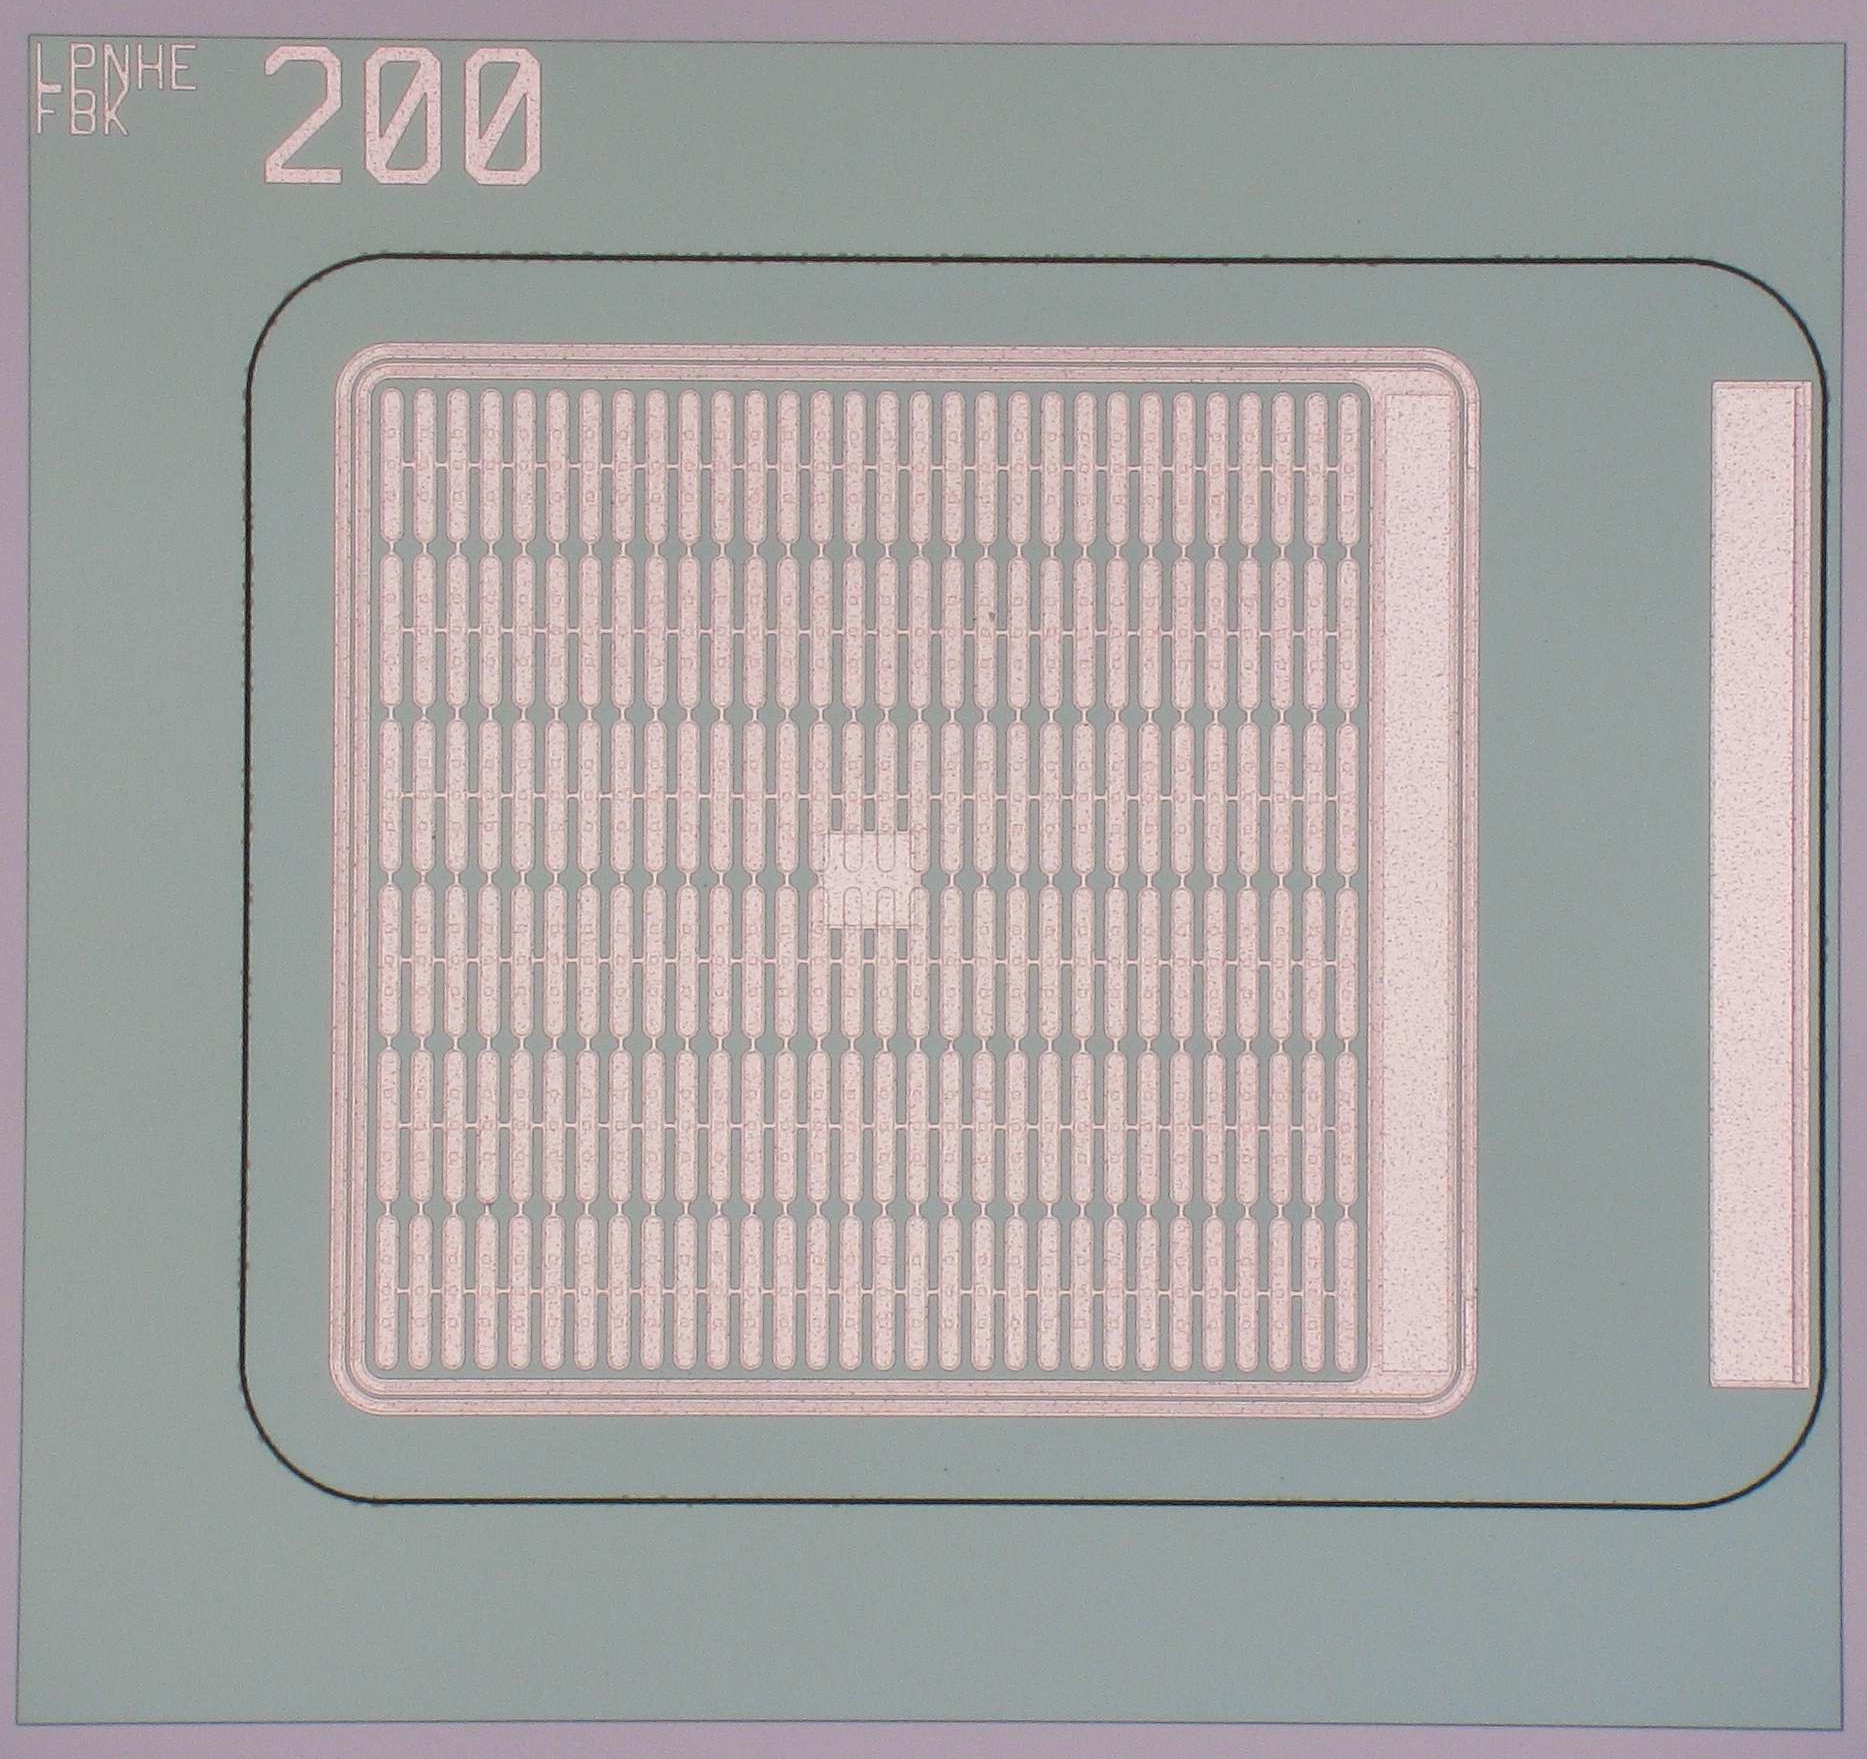
\includegraphics[height=0.335\textwidth]{testStruct.png}
\caption{\label{fig:pix_cap_struct}Left: test structures consisting of 2 arrays of 9~$\times$~13 FE-I4-like pixel cells each (``interpixel structure'');
the pixels in the left (right) structure have (no) field-plate.
Right: test structures consisting of an array of 6~$\times$~30 FE-I4-like
 pixel cells (``FE-I4 test structure''), where  all the pixels were shorted together.}
\end{center}
\end{figure}

 A test structure consisting of an array
 of 9~$\times$~13 FE-I4-like pixel cells was used to measure the interpixel  and the pixel-to-backside capacitance; the central pixel was isolated with respect to all the other pixels;
 the first 8 neighbours were shorted together, but isolated from all the other remaining (which, again,  were shorted together). These structures are shown on the
 left in Figure~\ref{fig:pix_cap_struct}, where two versions are present: one with metal field-plate and one without. ``Interpixel structure'' will be used for the sake of
 brevity in the remaining of the text to refer to this structure.


In Figure~\ref{fig:pix_cap_struct}, on the right, an array of 6~$\times$~30 FE-I4-like
 pixel cells is shown; all the pixels were shorted together allowing the measurement of the current voltage characteristics  of the whole array and of the inner GR (if present),
 and the break-down (BD) voltage dependence on
 the number of GRs and on the pixel-to-trench distance. Several combinations of values for the latter parameters are present on the wafer; in
 Figure~\ref{fig:pix_cap_struct}, on the right, a structure with a 200~$\mu$m pixel-to-trench distance and 2 GRs is shown. ``FE-I4 test structure'' will be used for the sake of
 brevity in the remaining of the text to refer to this structure.

For the interpixel structure, in Figure~\ref{fig:cv-testpixels}, the inverse of the square
 capacitance between all the pixels and the sensor backside is presented
 as a function of the bias voltage; the measurement was performed at a frequency of 10~kHz. From this measurement the sensors' depletion voltage was derived ($\sim$20~V).
For the same structure, in Figure~\ref{fig:cv-testpixels}, the capacitance between the central pixel and  all the other ones 
 is presented as a function of the bias voltage; the measurement has been carried out at three different frequencies $\nu$: 10, 100~kHz and 1~MHz.
  It can be seen that the presence of a field-plate increases the interpixel capacitance. The coupling is particularly important due 
 to the presence of the uniform p-spray implant. However, the level of capacitive coupling, even with  a field-plate, is acceptable in term of electronic noise for the read-out.



\begin{figure}[tbp]
\begin{center}
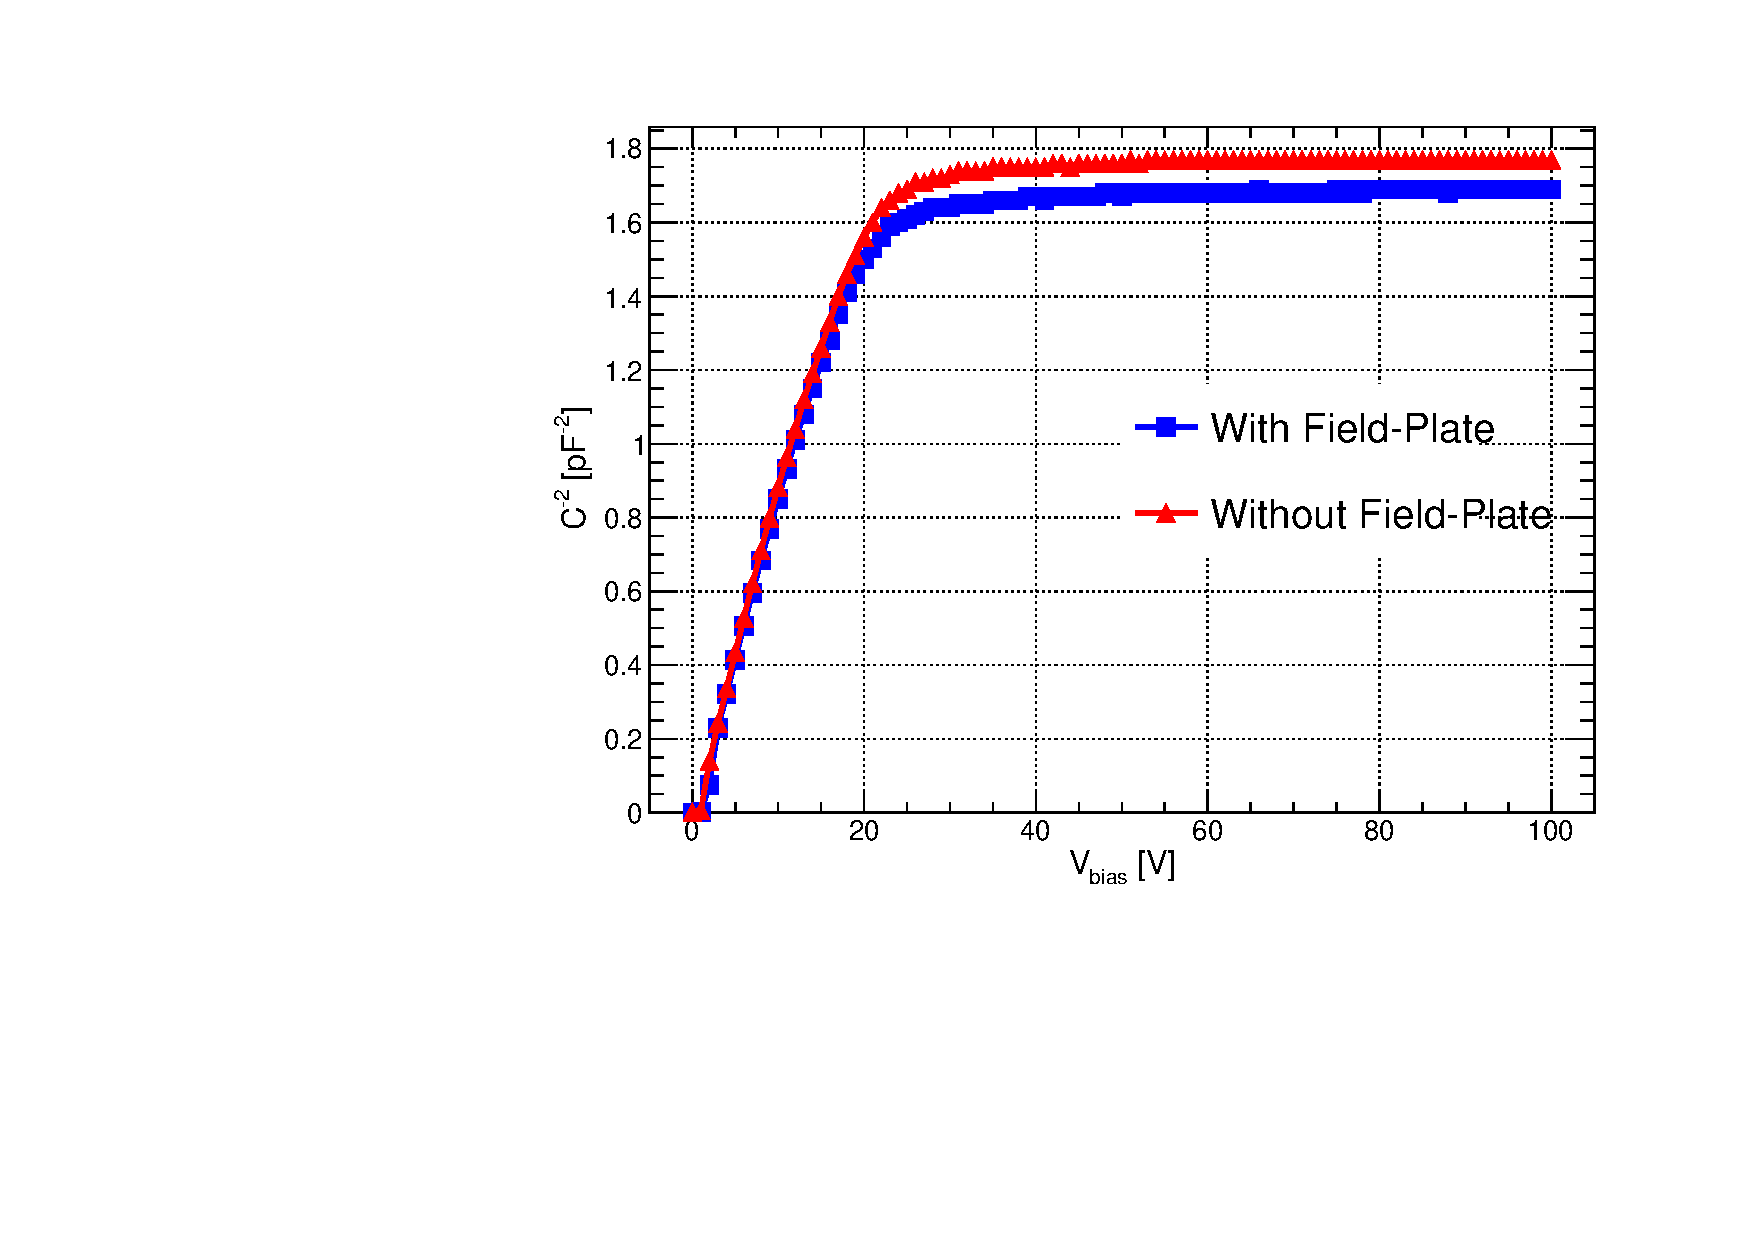
\includegraphics[width=0.49\textwidth]{edgelessC-2V.pdf}
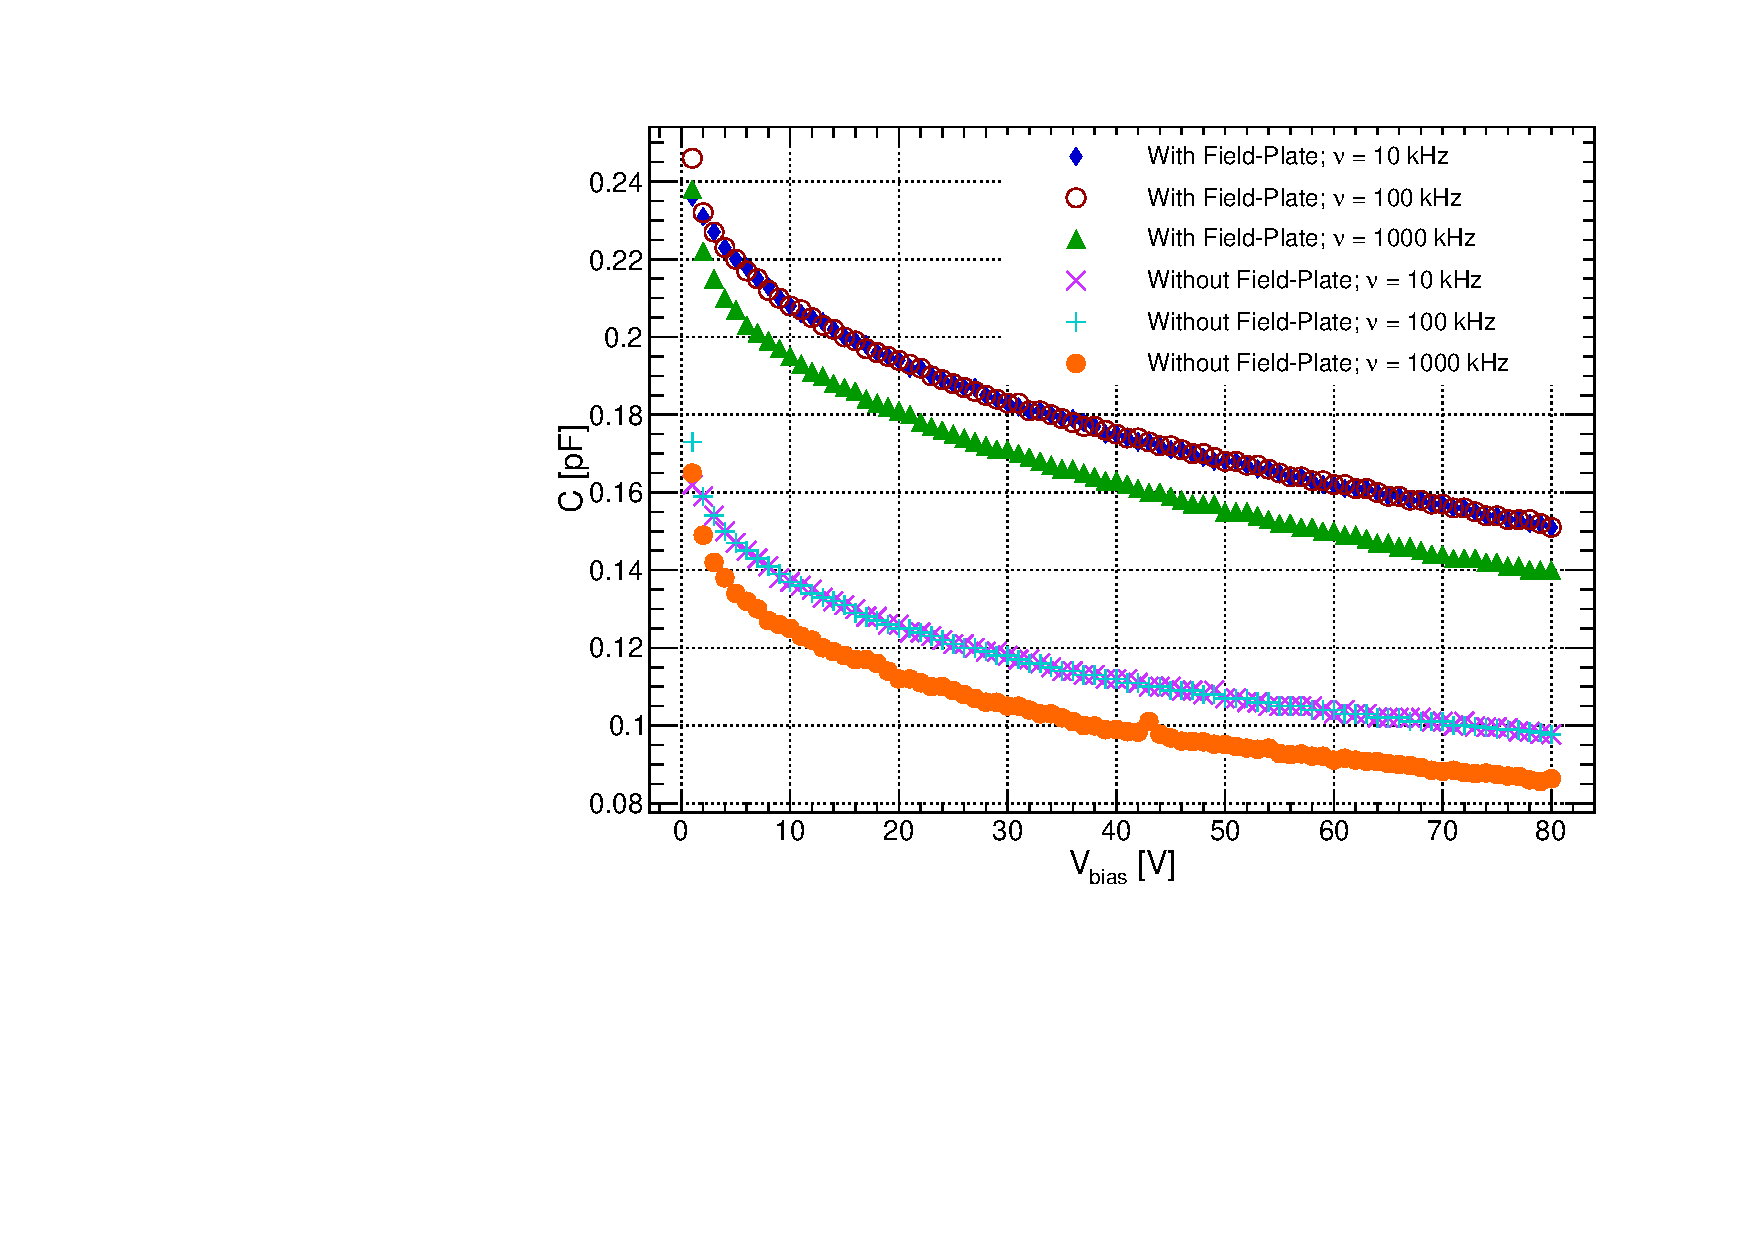
\includegraphics[width=0.49\textwidth]{edgelessInterpixelCV.pdf}
\caption{\label{fig:cv-testpixels}Measurements results for the intepixel structure; (left) inverse squared capacitance between all the  pixels and the sensor backside as a function of
the bias voltage; both pixels with  and without field-plate were tested; (right)
 interpixel capacitance for test structure with FEI4-like cells; the capacitance between the central pixel and
all the other pixels surrounding it in the test structure  is reported as a function of
the bias voltage for pixel cells with a field-plate, and
without it; the results are reported for three different frequencies: 10, 100~kHz and 1~MHz.}
\end{center}
\end{figure}

Using the interpixel structure  the interpixel resistance $\rm{R_{int}}$ was evaluated; the results are reported in Figure~\ref{fig:Rint} for the 2 different
p-spray doses. It can be seen that for the high p-spray dose value, at depletion voltage, the interpixel resistance is four times larger than  the low
p-spray dose corresponding value; nonetheless, excellent pixel isolation is already assured by low p-spray dose.
After irradiation, this test will be  crucial  to prove the pixels isolation.
\begin{figure}[!htbp]
\begin{center}
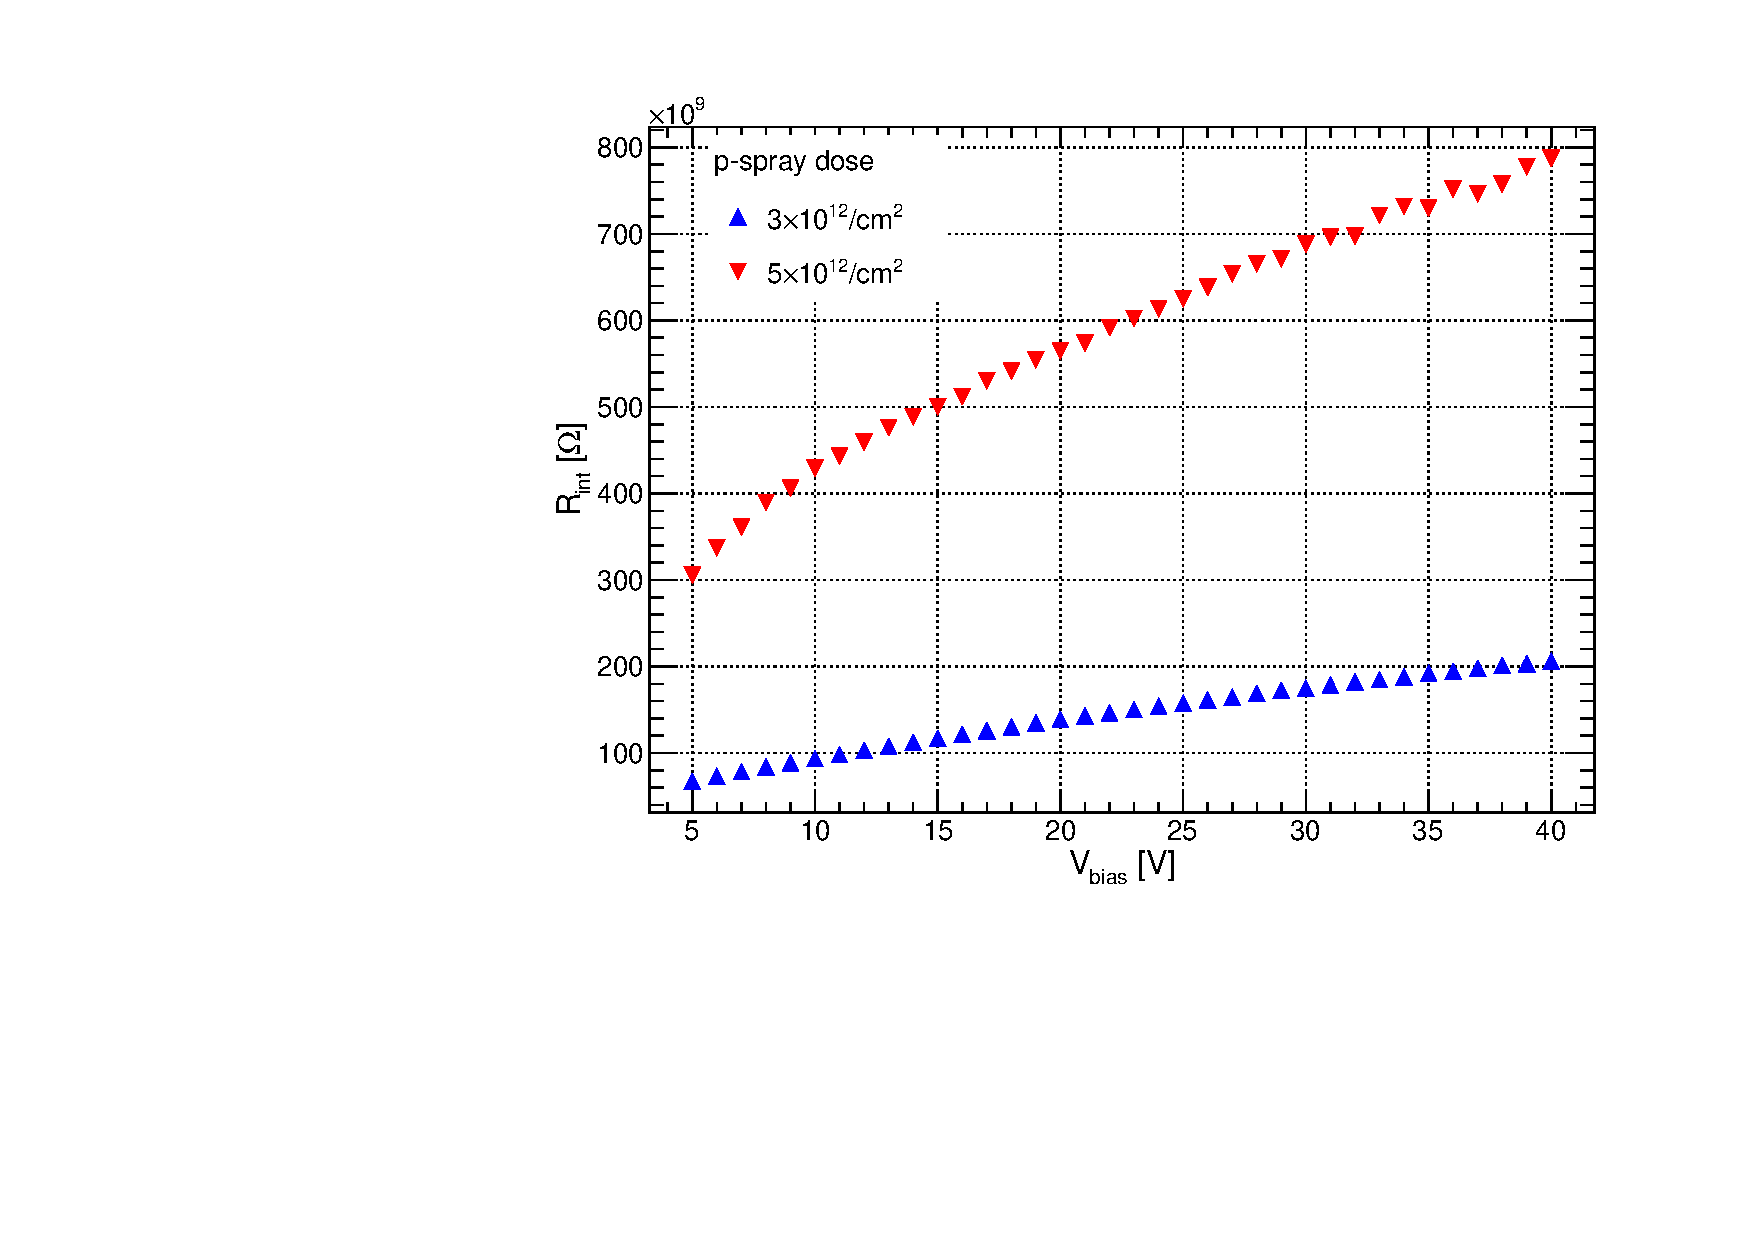
\includegraphics[width=0.44\textwidth]{edgelessabsCompareRint.pdf}
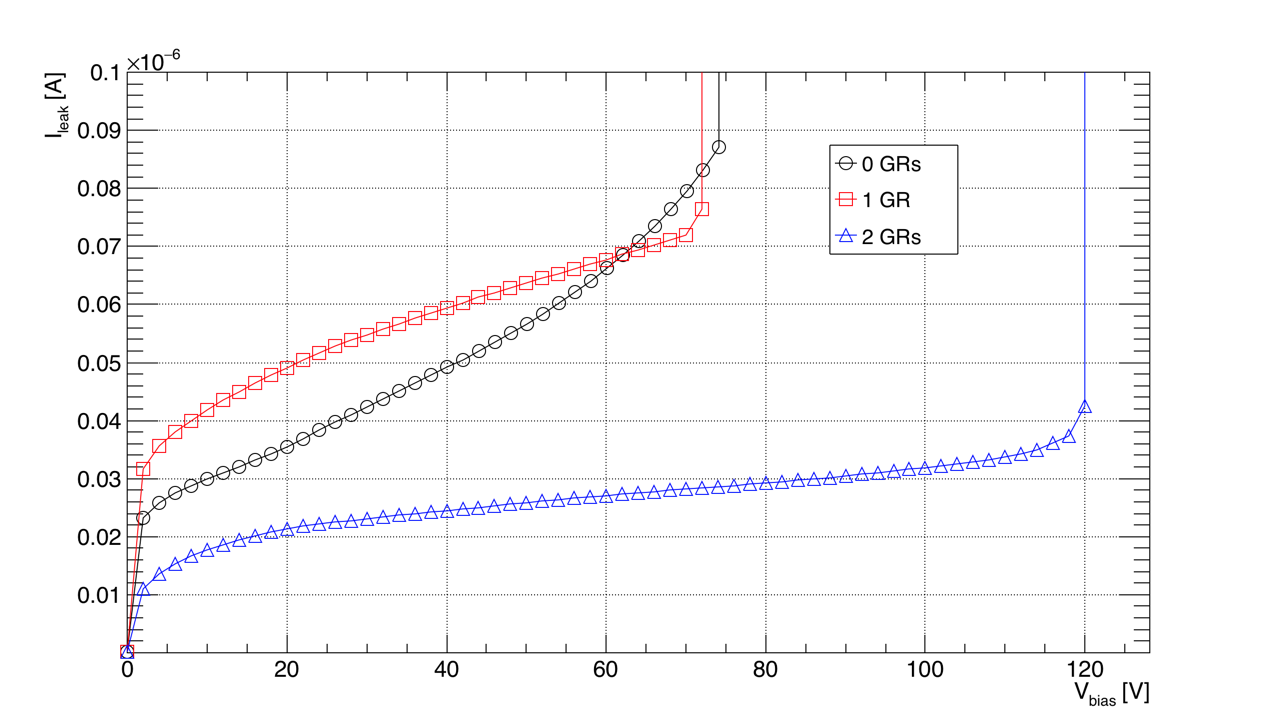
\includegraphics[width=0.55\textwidth]{W95_test_structures_ITOT_100um.png}
\caption{\label{fig:Rint}(left) Interpixel resistance $\rm{R_{int}}$ as a function of the bias voltage for two different p-spray doses. (right) Current-Voltage curves for
 test structures featuring different number of GRs. The
innermost GR, if present, was kept at ground voltage. The  shortest distance from the pixels to the trench is 100~$\mu m$. The measurement for the test structure with 2 GRs was taken at a lower temperature with respect to the other two samples.}
\end{center}
\end{figure}

 FE-I4 test structures  were used to evaluate the current voltage characteristics  of the production.
The effect of GRs on the breakdown voltage can be seen in Figure~\ref{fig:Rint},
where the current-voltage curves of test structures featuring FEI4-like pixels and different number of GRs are reported;  the distance between the last pixels and the doped trench is 100~$\mu m$~\cite{1748-0221-12-05-P05006}. The breakdown voltage increases by more than 70\% (from 70 to 120~V) by adding a second, floating GR.
%\begin{figure}[!htpb]
%\centering
%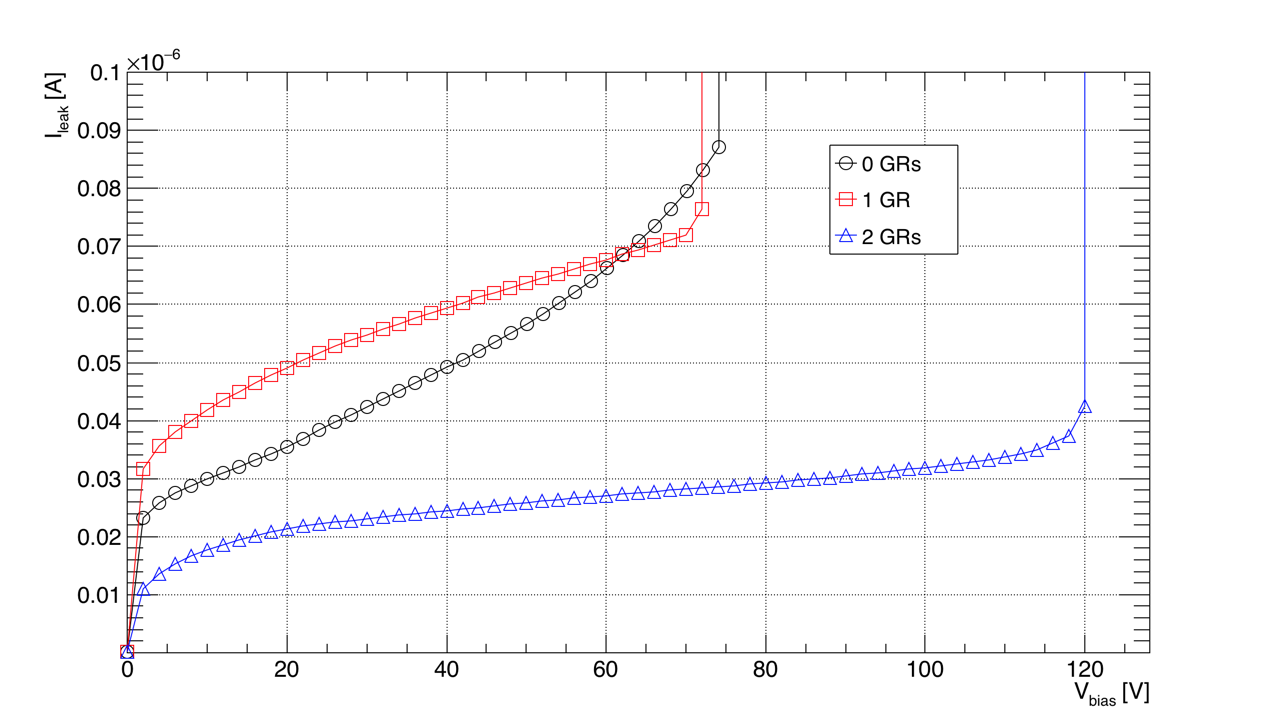
\includegraphics[width=0.65\textwidth]{W95_test_structures_ITOT_100um.png}
%\caption{\label{fig:IV_GRs}Current-Voltage curves for
 %test structures featuring different number of GRs. The
%innermost GR, if present, was kept at ground voltage. The  shortest distance from the pixels to the trench is 100~$\mu m$. The measurement for the test structure with 2 GRs was taken at a lower temperature with respect to the other two samples.}
%\end{figure}


\subsection{Beam test results}
Three sensors were bump-bonded to FE-I4 readout chips at IZM Berlin\footnote{Fraunhofer-Institut f\"ur Zuverl\"assigkeit und Microintegration: \url{https://www.izm.fraunhofer.de/en.html}} and were evaluated on beam~\cite{1748-0221-12-05-P05006}.

\subsubsection{Description of Tested Devices}
The main difference among the three sensors is  the number of guard rings (GRs) surrounding the active area, ranging from zero to two. In Figure~\ref{fig:lpnhe5_4_7_pic} a detail of the
sensor edge can be seen for all the three samples.

\begin{figure}[!htb]
\centering
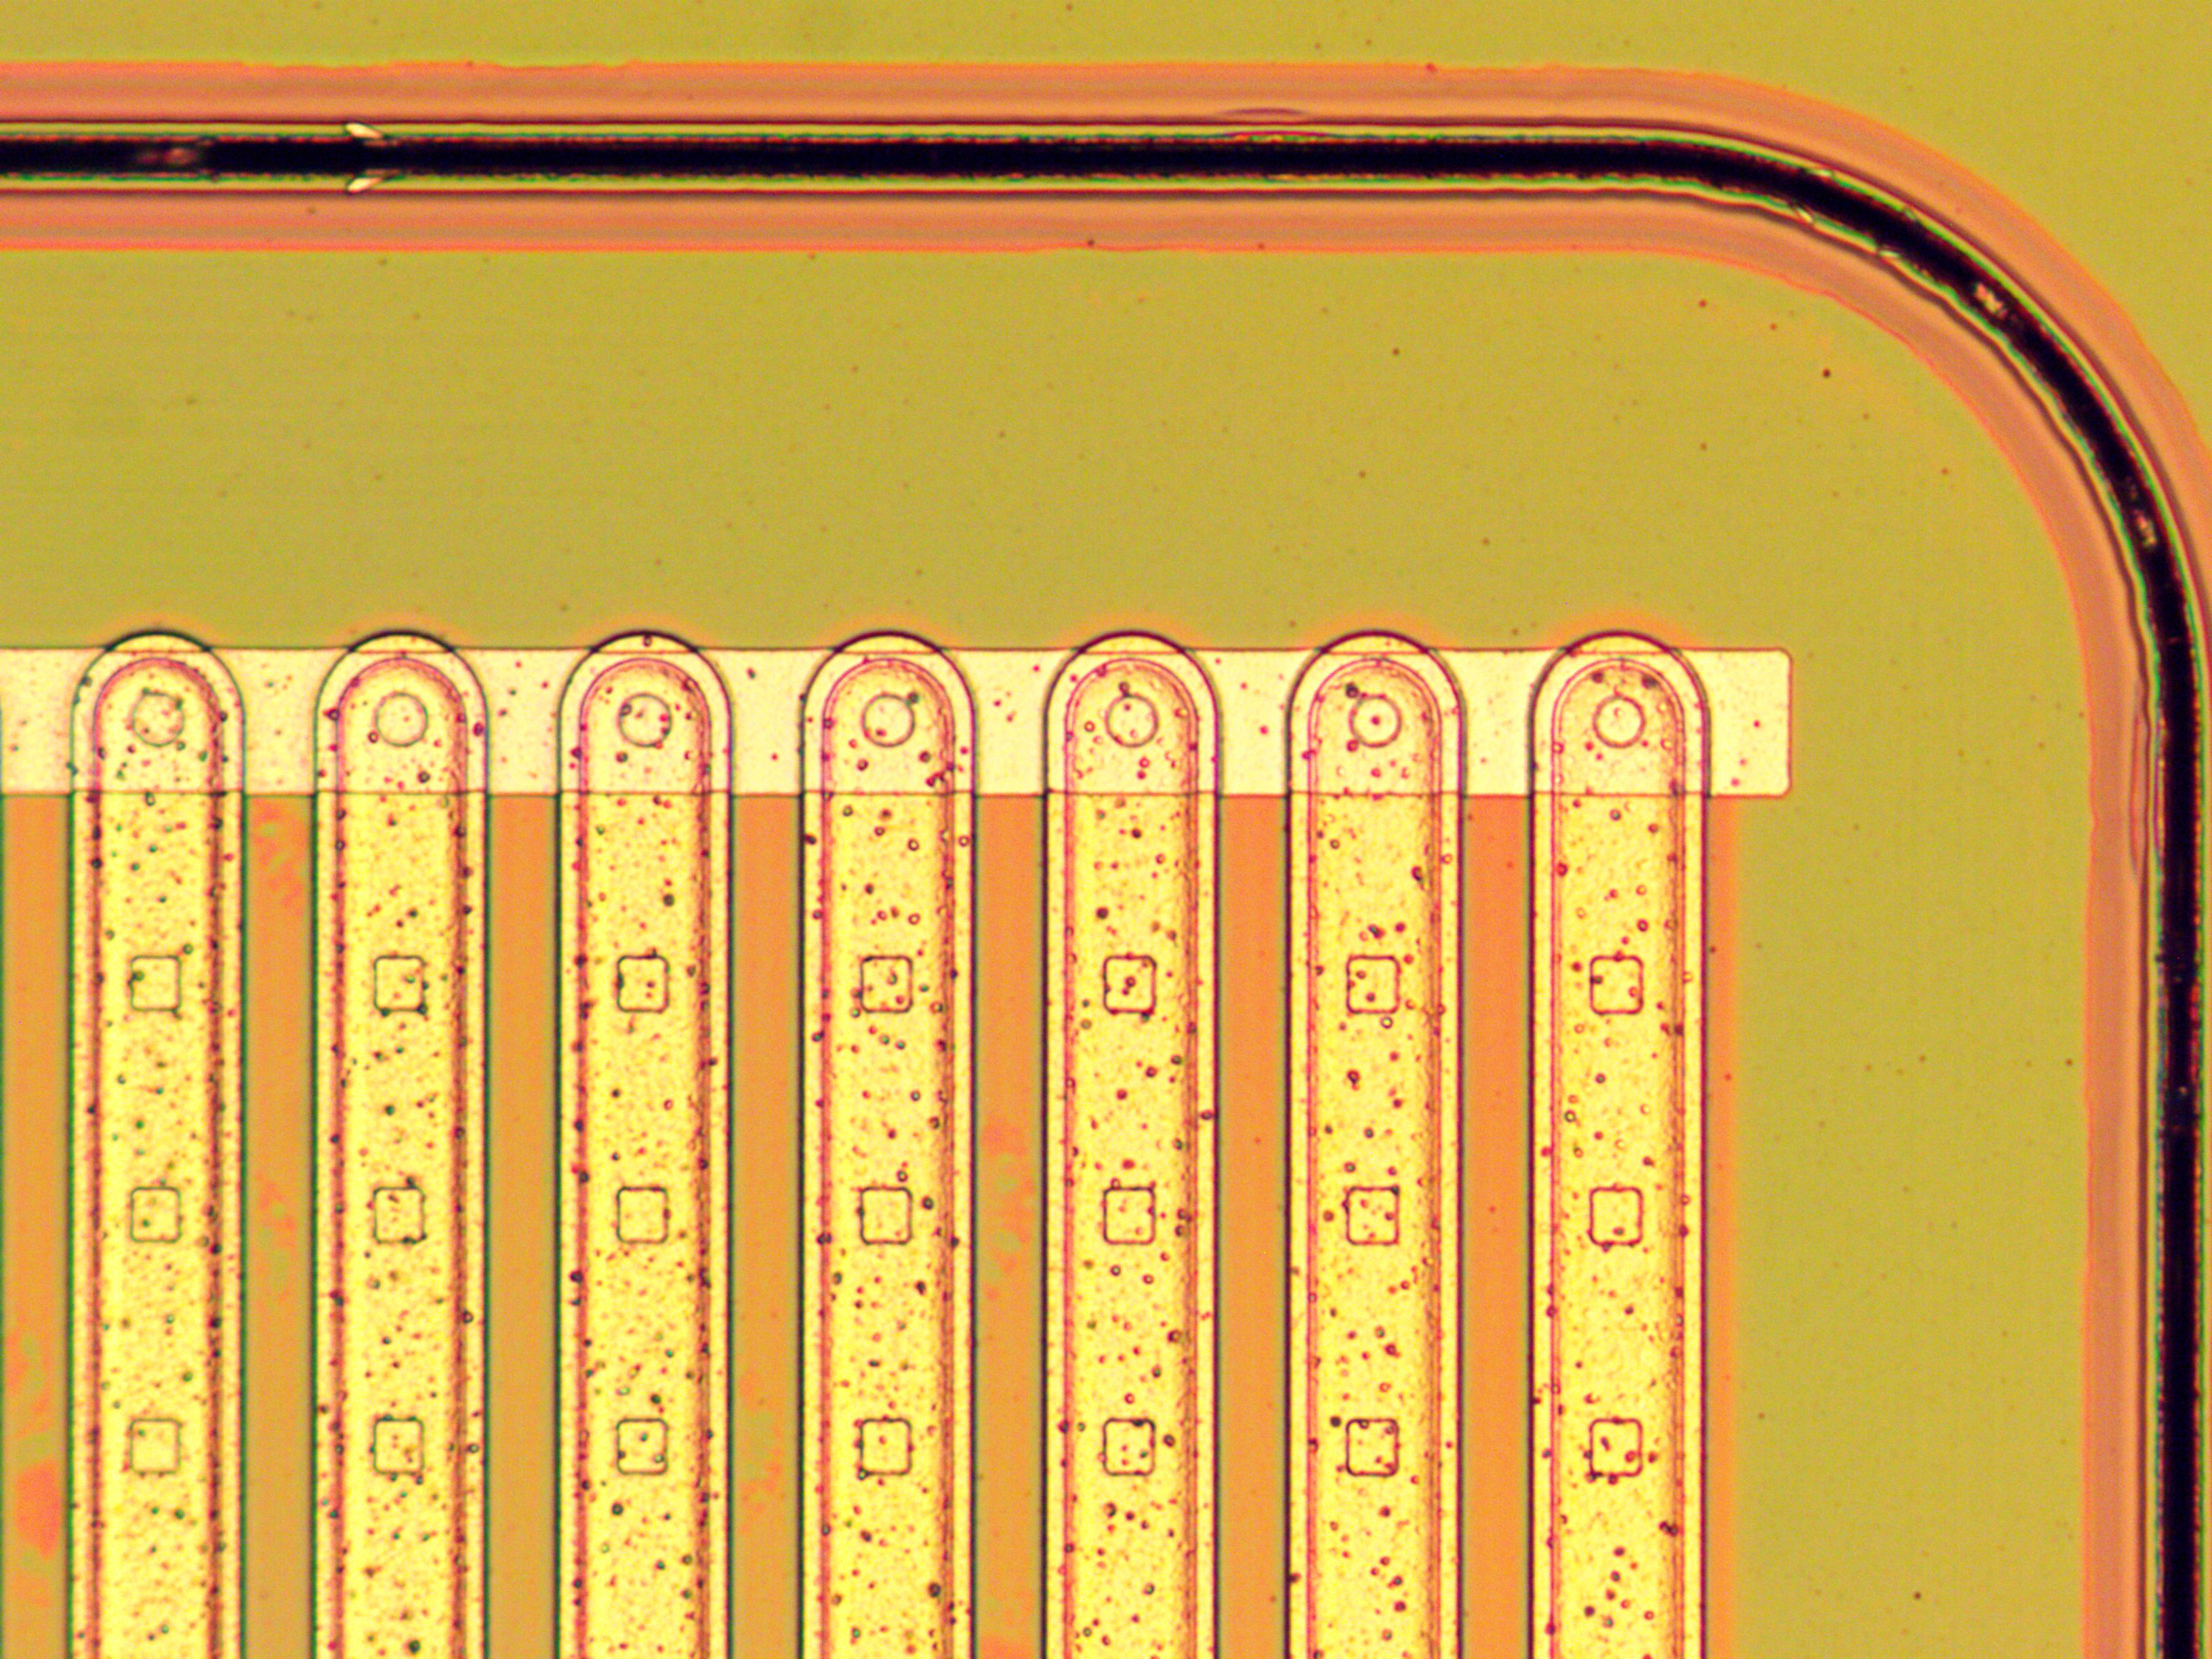
\includegraphics[width=0.30\textwidth]{fei4_100um_0GRs.jpeg}
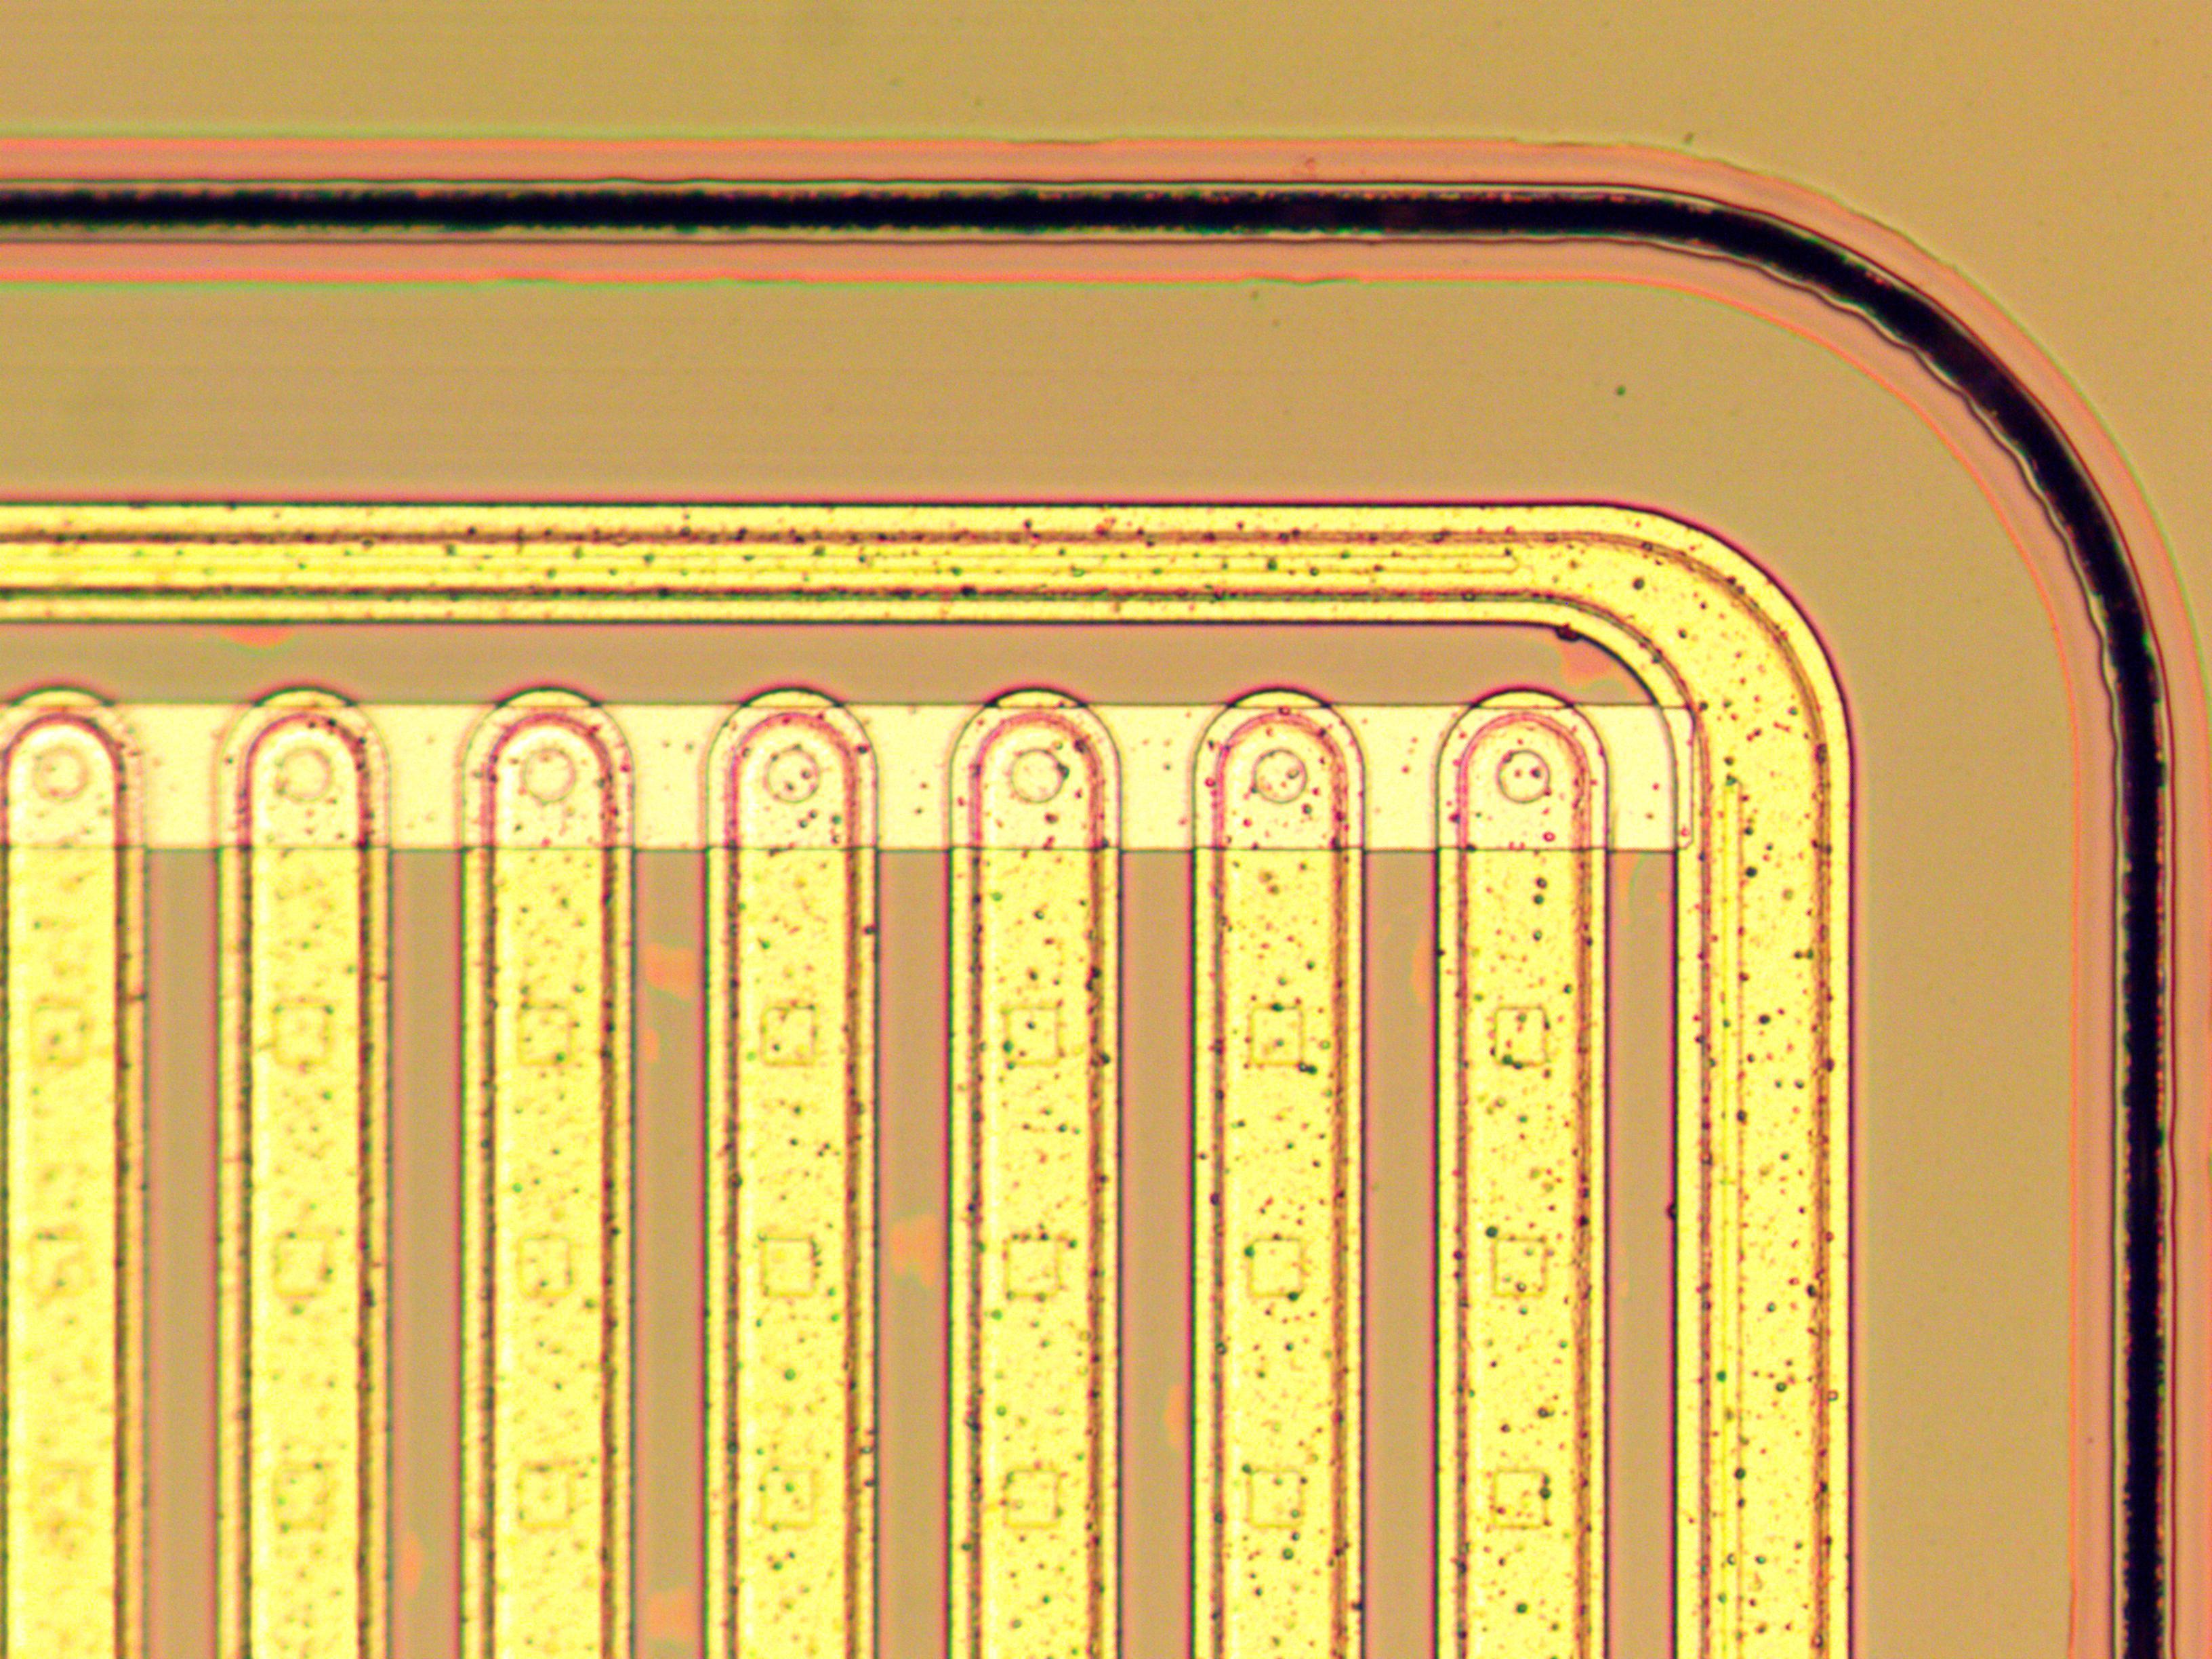
\includegraphics[width=0.30\textwidth]{fei4_100um_1GRs.jpeg}
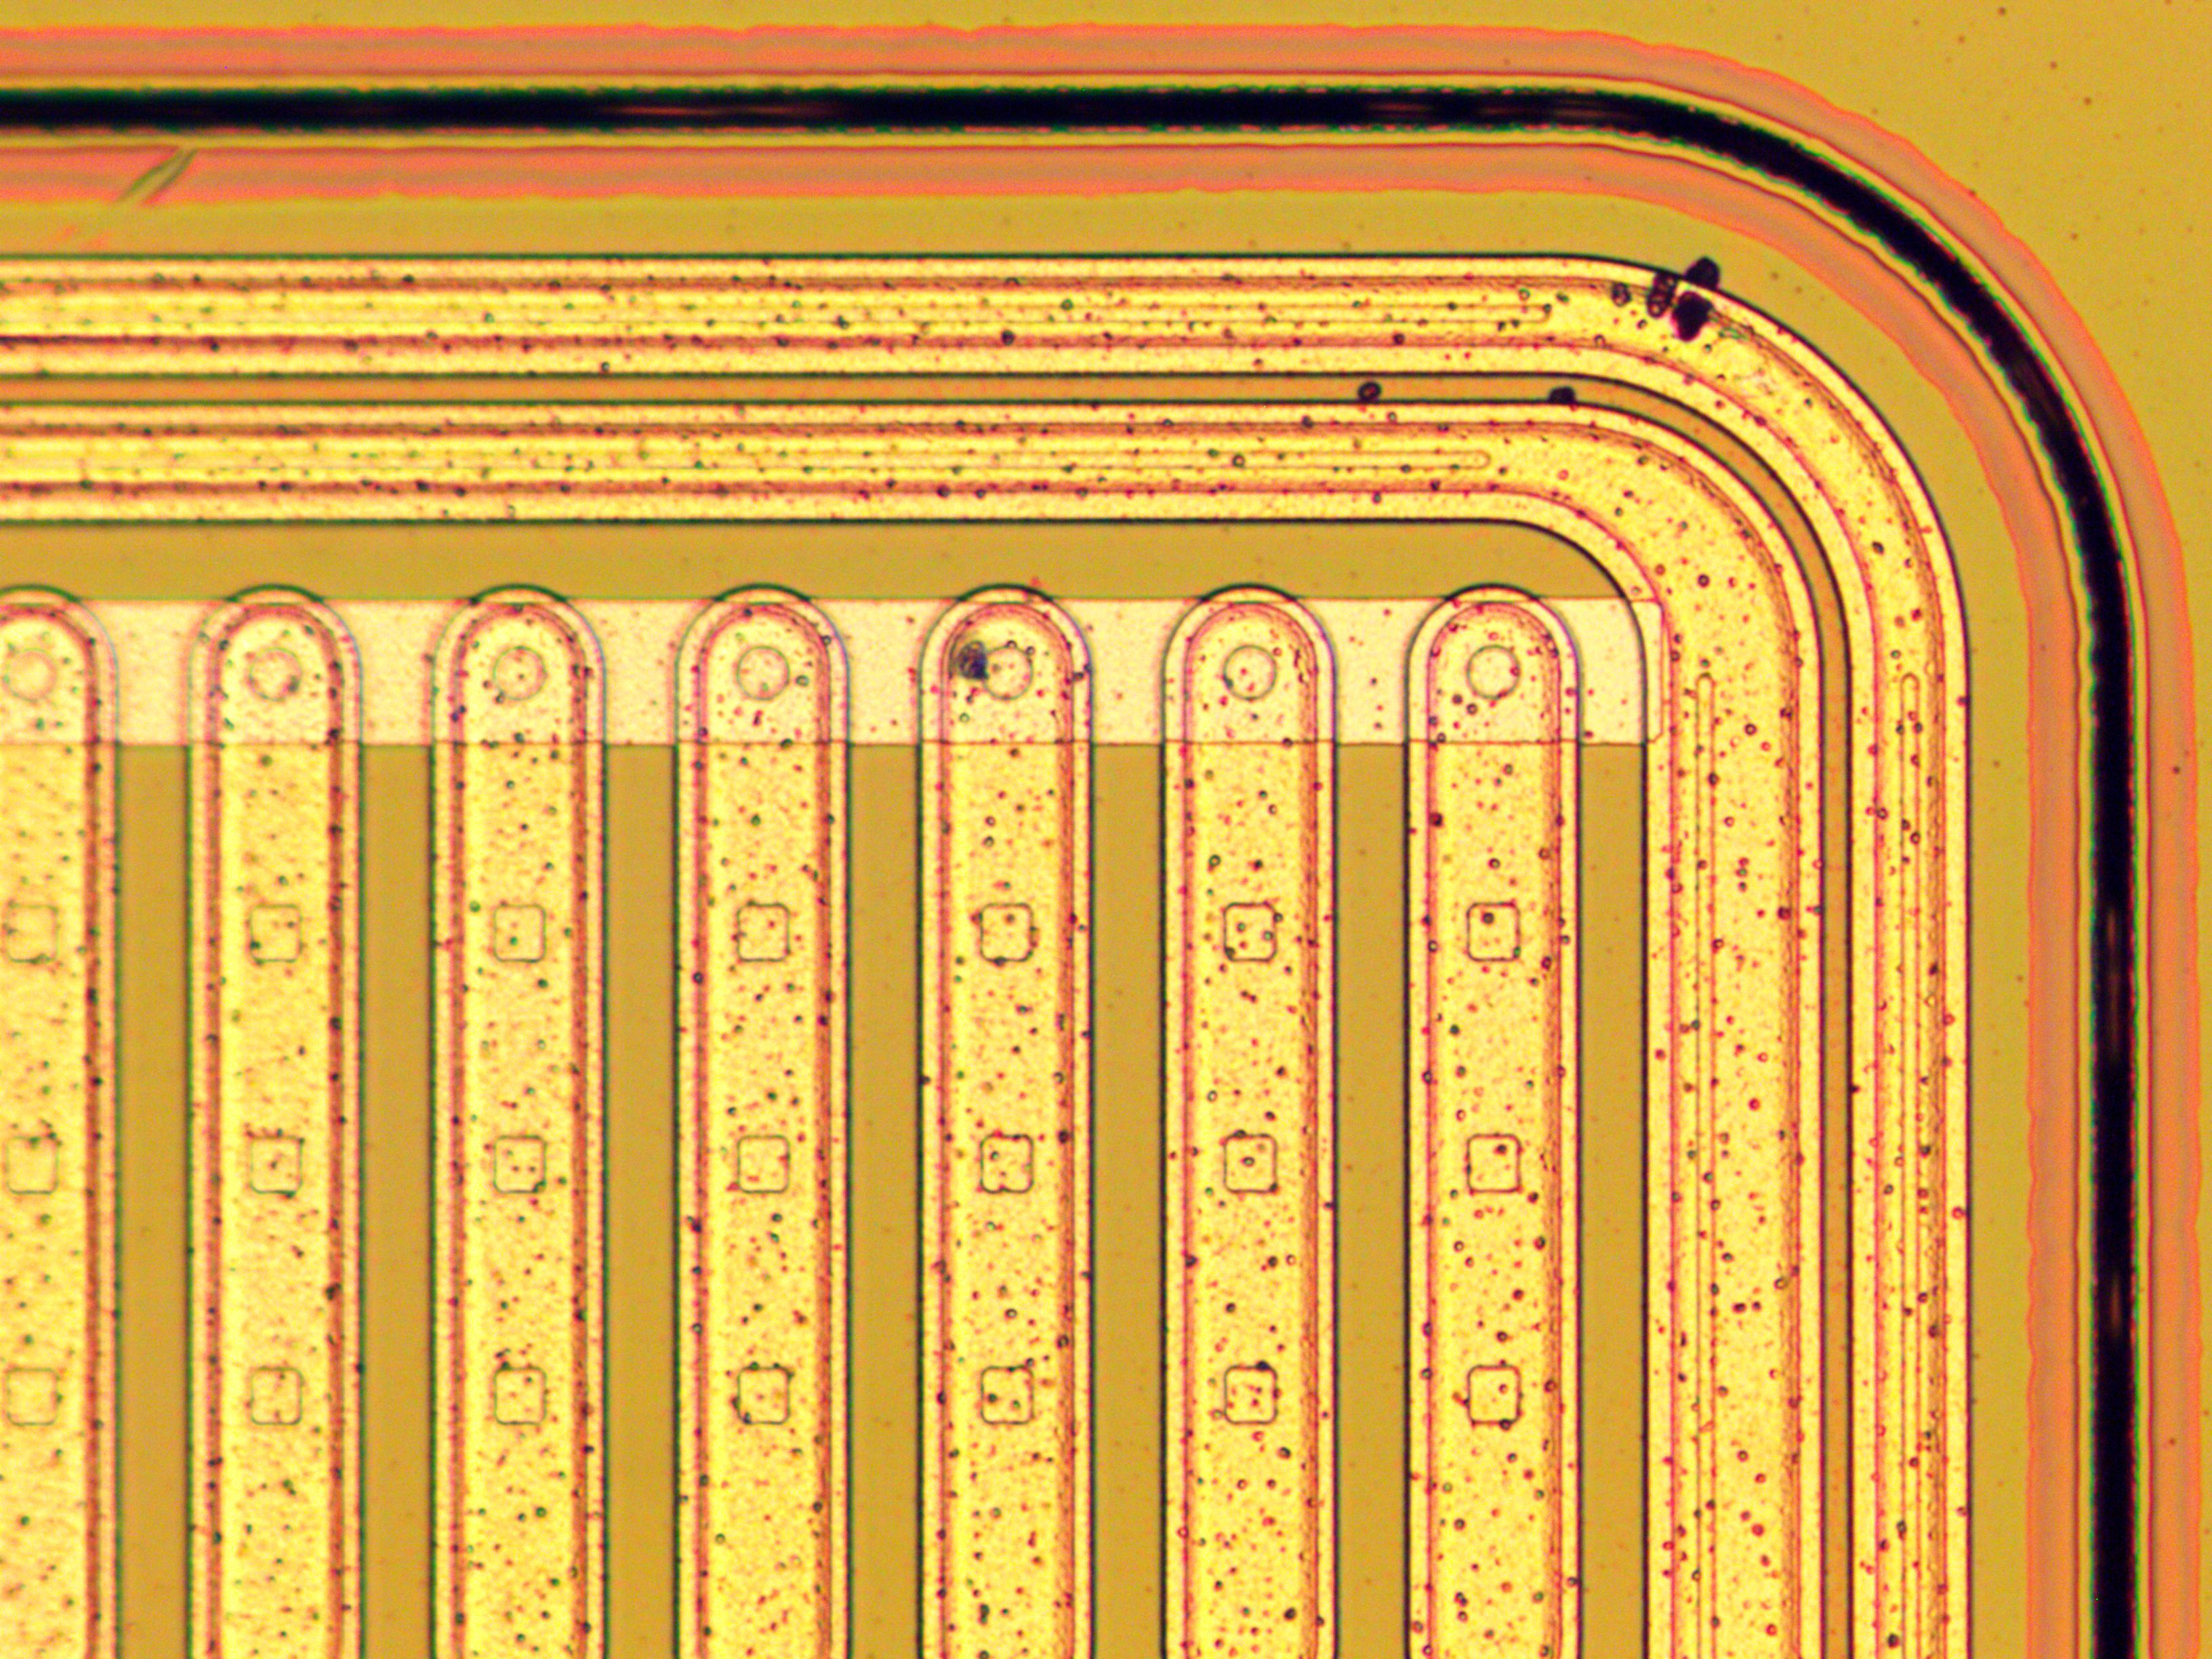
\includegraphics[width=0.30\textwidth]{fei4_100um_2GRs.jpeg}
\caption{\label{fig:lpnhe5_4_7_pic}Microscope picture of corners of the  (left) LPNHE5, (middle) LPNHE4  and (right) LPNHE7 sensor. The black line at the top and on the right is the trench. The  shortest distance from the pixels to the trench is 100~$\mu m$ for all the three sensors. For LPNHE4 there is  one GR surrounding the pixel matrix; for LPNHE7 there are two GRs. The pictures show also a temporary metal strip~\cite{bib:metal} shorting the pixels: it was used at wafer level for checking the sensor current  but it was removed from the detectors tested in this work.}
\end{figure}
LPNHE5 has no GRs, LPNHE4 has one GR and LPNHE7 has two GRs. All sensors are 200~$\mu$m thick $n-on-p$ and include a uniform p-spray implant on the pixels side to provide enough insulation among them. LPNHE4 and LPNHE5 sensors have, in addition, p-stops implants that surround the implants of pixels and GRs.
The main  characteristics of the devices are summarized in Table~\ref{tab:device_charact}.

\begin{table}[!htbp]
\centering
\caption{\label{tab:device_charact}Tested devices characteristics.}
\smallskip
\begin{tabular}{lcc}
\hline
\hline
Name&Number of GRs& p-stop implant\\
\hline
LPNHE5 & 0 & yes\\
LPNHE4 & 1 & yes\\
LPNHE7 & 2 & no\\
\hline
\end{tabular}
\end{table}


The LPNHE4 module was used in an irradiation experiment before the beam tests. Laboratory measurements after irradiation showed that, due to the lack of  electrical insulation layer
between the sensor and the FEI4-B readout chip (for a discussion of this issue see for example~\cite{rossi2006pixel}), it couldn't be biased up to full depletion. Hence there are not be
beam test results for irradiated detectors from this pixel sensors production but only laboratory 
measurements with radioactive sources which will be presented at the end of the Section.


During all measurements the innermost GR, if present, was kept at
 ground voltage by the FE-I4 readout chip; the second GR, when present, was left floating. The depletion voltage for all three devices was about 20~V.

\subsubsection{Detector Configuration and Experimental Setup}
Before laboratory and beam tests the threshold and gain settings of the readout electronics are carefully tuned. When choosing the threshold, a compromise has to be found between a high threshold, which decreases the number of noise hits but decreases the signal efficiency as well, and a low threshold, with opposite effects. For our detectors, a typical threshold is 1400~e, which corresponds to a tenth of the expected most probable value signal amplitude due to a minimum ionizing particle (MIP) crossing the sensor at normal incident angle. A typical result from  threshold tuning\cite{FEI4,USBpix} can be see in Figure~\ref{fig:threshold}; the threshold dispersion is of the order 200~e. The signal amplitude in the sensor is measured in  units of Time over Threshold (ToT): a clock counts when the shaped signal  goes above threshold and stops when the signal falls below threshold; the difference between those two crossings is the ToT~\cite{FEI4}. During the tuning of the electronics, the correspondence between ToT value and input charge is calibrated.\\
\begin{figure}[!htb]
\centering
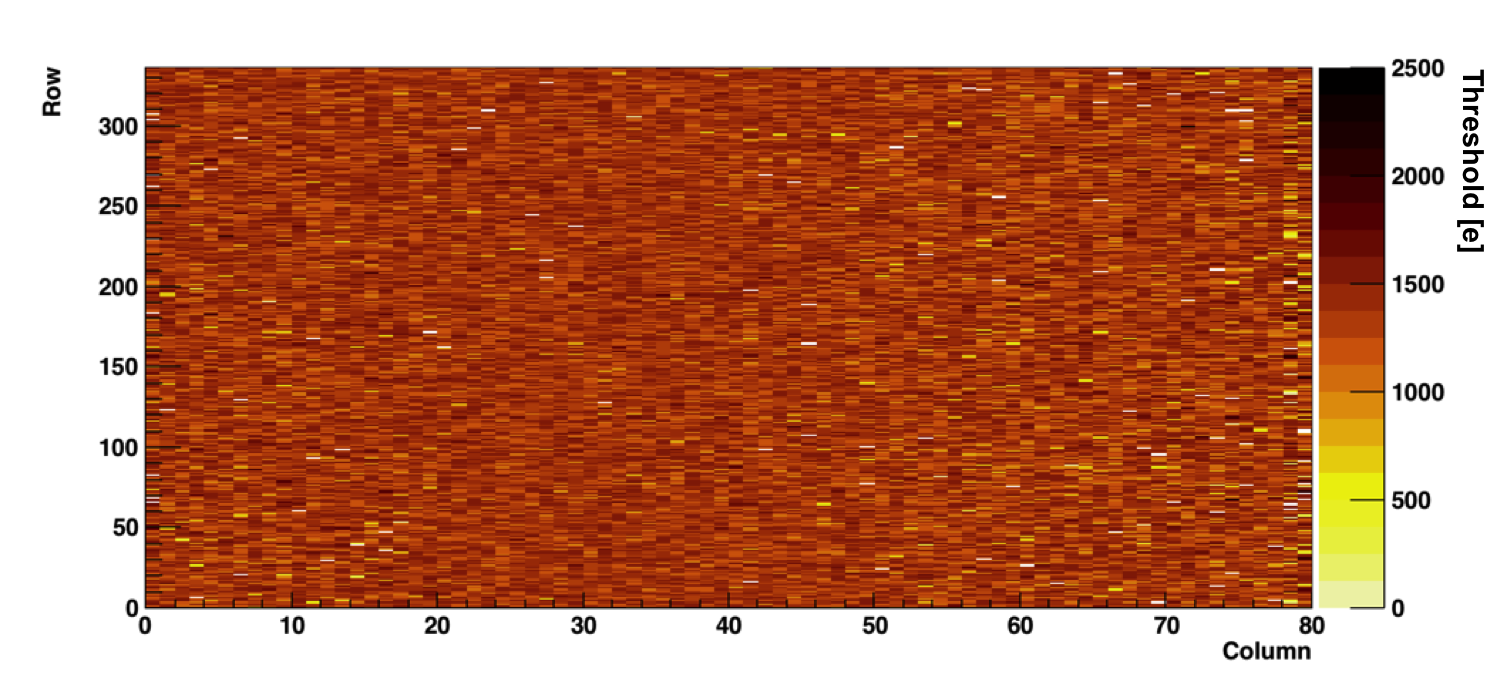
\includegraphics[width=0.65\textwidth]{lpnhe7_threshold_40V.png}
\caption{\label{fig:threshold}Pixel threshold values for LPNHE7. On the abscissa is the pixel column index, on the ordinate axis is the pixel row index.
The tuning target value was 1400~e; the sensor bias voltage was 40~V.}
\end{figure}


The results presented here are based on data
taken at the DESY beam test facility\footnote{http://testbeam.desy.de/} and at the CERN
North Area experimental area\footnote{http://sba.web.cern.ch/sba/}.
At DESY 4~GeV/c momentum electrons were used; at CERN 120~GeV/c momentum positive pions were used.


At both laboratories the data were recorded using a copy of the Eudet/AIDA telescope~\cite{Jansen2016} 
already presented elsewhere. 
The data from the DUTs were recorded using two different Data Acquisition (DAQ) systems: the 
Reconfigurable Cluster Element (RCE)~\cite{RCE} system and the UsbPix~\cite{USBpix} system.
The typical averaged\footnote{Averaged over a supercycle at CERN} trigger rate was in the range of 
250-1000~Hz, depending on the
beam conditions and on the DAQ system used for the devices under test (DUTs).



The DUTs were located between the two arms of the telescope (each arm having three detection planes). To screen the DUTs from the light, they were operated inside a cooling box, capable  of maintaining the DUT temperature constant.

\subsubsection{Data Reconstruction and Analysis}

Raw data were processed into tracks using the algorithms implemented in the EUTelescope 
framework~\cite{eutelescope}.
At the end of the process a ROOT~\cite{root} file is created containing basic observables  ready to be analyzed in the data analysis framework, TBmon2 software~\cite{tbmon2}.
TBmon2 allows studying the quantities discussed below.

\paragraph{Global, In-Pixel and Edge Hit Efficiency}
The global hit efficiency is defined as the  fraction of reconstructed tracks crossing a sensor that have an associated hit in that sensor. A bad bump bonding can degrade severely the efficiency of the sensor.
The quoted efficiency is measured in a fiducial region, defined by the surface of the pixel module where each pixel cell is
hit by at least 1 track. From Figure~\ref{fig:hitmap} it can be seen that the fiducial region,  defined by the trigger scintillators area, is smaller than the surface of the detector. Nonetheless
the uniformity in threshold show in Figure~\ref{fig:threshold} is a good
indication that the performance measured in the fiducial area can be taken as valid also outside it,
hence the hit efficiency be interpreted as global.

\begin{figure}[htbp]
\centering % \begin{center}/\end{center} takes some additional vertical space
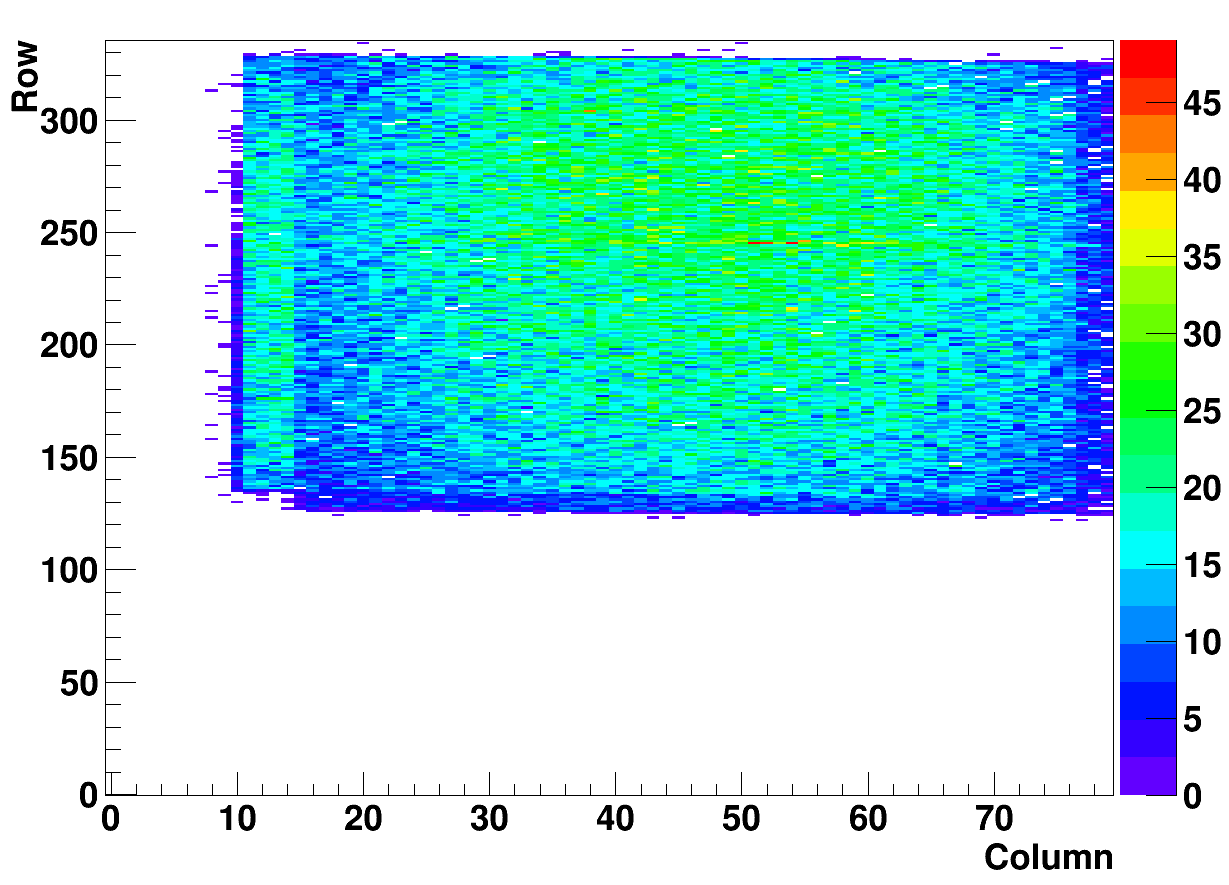
\includegraphics[width=.45\textwidth,origin=c,angle=0]{hitmap_center.png}
\qquad
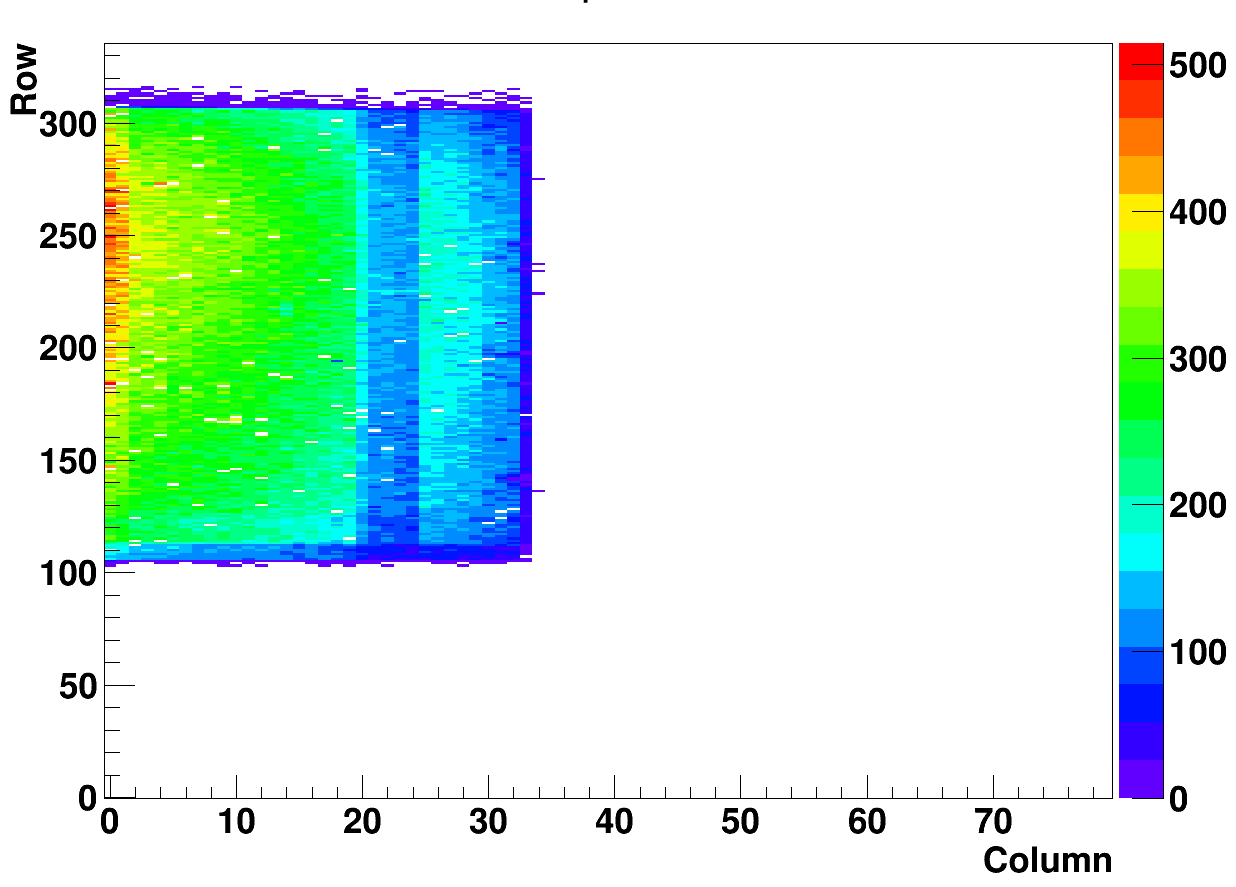
\includegraphics[width=.45\textwidth,origin=c,angle=0]{hitmap_edge.png}
% "\includegraphics" from the "graphicx" permits to crop (trim+clip)
% and rotate (angle) and image (and much more)
\caption{\label{fig:hitmap} Hit map of a tested sensor in beam. On the abscissa is the pixel column index, on the ordinate axis is the pixel row index. (Left) the beam is focused on the center of the sensor; (right) the beam  is focused on the edge, which allows to perform edge efficiency scan. The area where hits are seen is a 1 $ cm^2$ rectangle and correspond to the area of the trigger scintillator.}
\end{figure}

The in-pixel hit efficiency is obtained by superimposing the 2D maps of efficiency as a function of the local position in each pixel cell of the sensor, the granularity of this analysis being of the order of the total pointing resolution (sum of the telescope resolution and the multiple scattering average shift). The in-pixel efficiency gives valuable information on the homogeneity of the charge collection, stressing the presence of low efficiency areas due, for instance, to permanent biasing structures. Our sensors do not include permanent biasing structures, since for testing purposes they are polarized thanks to a temporary metal line~\cite{bib:metal}, which is then removed before bump bonding.

To assess whether the active edge ensures a high hit efficiency in the  area between the last pixels and the doped trench, an efficiency measurement as a function of the track position in the edge area is performed, using data collected with the beam focused on the edge area; see also Figure~\ref{fig:hitmap}.
The impact of the GRs on the efficiency is studied by comparing numerical device simulations with the edge hit efficiency profiles. The lateral depletion can be investigated looking at the edge efficiency performance
 for several values of the bias voltage.

\subsubsection{Efficiency Results for the Edgeless Sensors}

In what follows the global hit, in-pixel and edge hit efficiency results from the beam tests  will be presented.

\paragraph{Global Hit Efficiency}
\begin{figure}[htbp]
\centering % \begin{center}/\end{center} takes some additional vertical space
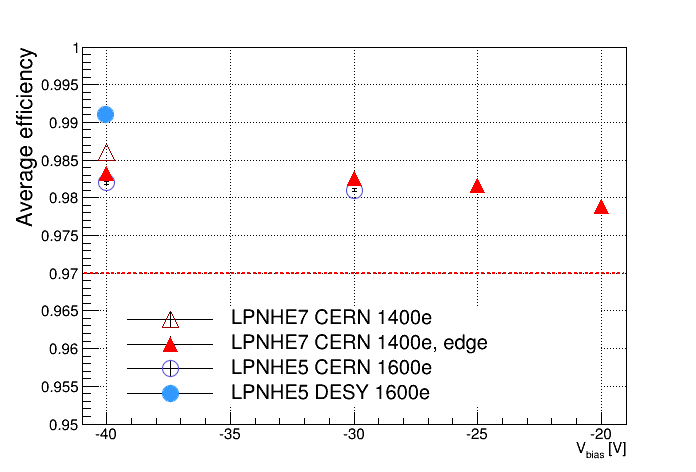
\includegraphics[width=.65\textwidth,origin=c,angle=0]{eff_open.png}

% "\includegraphics" from the "graphicx" permits to crop (trim+clip)
% and rotate (angle) and image (and much more)
\caption{\label{fig:eff} Global hit efficiency for the 2 sensors (LPNHE7 and LPNHE5), for various bias points, threshold configurations (1600 e or 1400e ) and beam tests (CERN or DESY). ``Edge'' identifies data taken when the
beam was focused at the detector periphery.}



\end{figure}

The hit efficiency has been investigated at CERN SPS and DESY with a set of two thresholds corresponding to an input charge of 1400 electrons or 1600 electrons and for various bias points.
The global hit efficiency is higher than 97.5 $\%$ for both the LPNHE5 and LPNHE7 sensors, as shown in Figure~\ref{fig:eff}.
For LPNHE7 at the CERN SPS with a threshold of 1400 electrons, two beam configurations were investigated, one with the beam focused on the center of the sensor (open triangles), the other with the beam focused on the edge of the sensor (full triangles).
Biasing the sensor above 25~V allows the sensors to reach a 98~$\%$ efficiency whatever the threshold.

\paragraph{In-Pixel Hit Efficiency}


\begin{figure}[htbp]
\centering % \begin{center}/\end{center} takes some additional vertical space
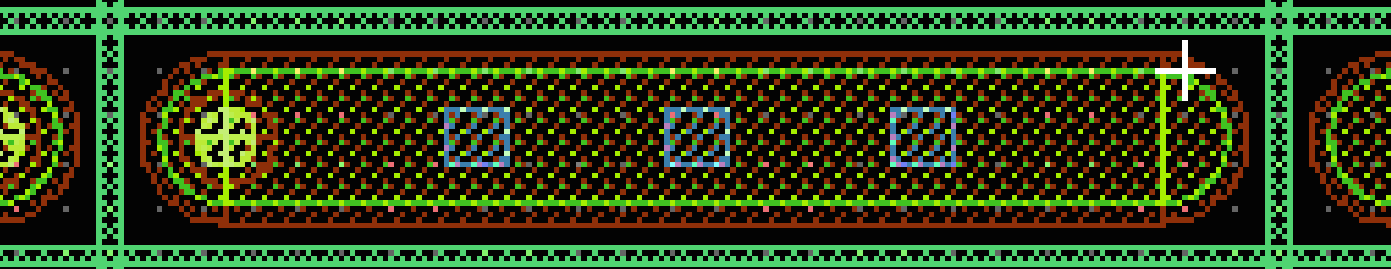
\includegraphics[width=.7\textwidth,origin=c,angle=0]{rsz_schemepix.png}

\includegraphics[width=.75\textwidth,origin=c,angle=0]{pixeff-center.png}
% "\includegraphics" from the "graphicx" permits to crop (trim+clip)
% and rotate (angle) and image (and much more)
\caption{\label{fig:pix} Pixel scheme (top) with inner structures: n$^+$-implant, metal contacts, bump bond pad, p-stop... and in pixel efficiency (bottom) for LPNHE7 at 40~V.}


\end{figure}
As observed in Figure \ref{fig:pix}, the in-pixel efficiency is very homogeneous. This high homogeneity shows the interest of using a temporary metal to bias the sensors for electrical tests before bump-bonding instead of adding a permanent structure such as punch-through bias dots. A tiny drop of efficiency can be observed at the pixel corner, where it decreases to  95$\%$. This is due to the charge sharing occurring between 3 or 4 neighboring pixels. In those clusters, the charge induced in one of the pixels could be under threshold and then not taken into account, which biases the hit reconstruction and the hit efficiency.

This result is to be compared to the one in Figure~\ref{fig:n-in-n:Oct_P5_D11_qeff} where charge is lost 
in the bias grid area and Figure~\ref{fig:NPTW80InpixelEff.pdf} where the bias rail is responsible for 
lower hit efficiency.

\paragraph{Edge Efficiency}
The hit efficiency at the detector edge for both LPNHE5 and LPNHE7 is presented in Figure \ref{fig:edge_comparison}. LPNHE5 and LPNHE7 were measured at DESY and at CERN respectively; the threshold was set to 1600~(1400)~e for LPNHE5 (LPNHE7), while the bias voltage was 40~V for both detectors.
\begin{figure}[!htbp]
\centering 
\includegraphics[width=0.75\textwidth,origin=c,angle=0]{edgeeff_full_range_pics.png}
\caption{\label{fig:edge_comparison}
Edge efficiency profiles for  LPNHE5 (no GRs - full markers) and LPNHE7 (2 GRs - open markers). Laboratory were the data were taken, device bias voltage and threshold are indicated too. The horizontal dashed line marks the
50\%-point efficiency. The devices photograph on top helps in visualizing which physical area of the pixel is related to the efficiency profile.}
\end{figure}

Thanks to the active edge technology both detectors are efficient even in the un-instrumented area: for both LPNHE5 and LPNHE7 the efficiency is higher than 50$\%$ up to about 90 $\mu m$ away from the last pixel, that is only 10 $\mu m$ from the cut edge. This performance meets the specifications of ATLAS ITk pixel modules~\cite{ITkStripsTDR} in terms of distance from the active region to the cut edge.

As a reminder, LPNHE7 has 2 GRs, one connected to ground laying between 13~$\mu m$ and 50~$\mu m$ from the last pixel, one floating between 55~$\mu m$ and 80~$\mu m$; LPNHE5 has no GRs.
The behavior of the 2 samples is rather similar in the first 30~$\mu m$, where the efficiency is basically flat. Then the efficiency  drops faster  for LPNHE5, while  for LPNHE7 the efficiency is a plateau between 0 and -50~$\mu m$ then it smoothly decreases to reach 90~$\%$ at -80~$\mu m$, before sharply dropping to 0.

Even if data taking conditions were different and clearly sub-optimal for LPNHE5 (higher threshold, multiple scattering,~...), the detector is still quite efficient in the edge area. In particular, it is to be noted that the slope of the hit efficiency curve is consistent with the smearing in the telescope tracking resolution due to the multiple scattering. Nevertheless, further tests on active edge sensors without GRs are necessary, with better experimental conditions.

For LPNHE7, the good performance in terms of efficiency in the edge area indicates that the presence of GRs does not degrade too much the  hit efficiency, even in the area of the innermost connected GR.


To better understand the efficiency in the GRs region,, two dimensional numerical simulations (for details see~\cite{bib:nim2012}) were run; the edge area of  sensors with 0 and 2 GRs and
a 100~$\mu m$ distance between the last pixel
and the doped trench were studied. The results are shown in Figure~\ref{fig:EFtcad_edge} for a simulated bias voltage value of 40~V.

\begin{figure}[!htbp]
\centering
\includegraphics[width=0.497\textwidth,origin=c,angle=0]{smaller2GR_0.png}
\includegraphics[width=0.497\textwidth,origin=c,angle=0]{GR_2.png}
\caption{\label{fig:EFtcad_edge}Numerical simulation  of the electric field. Left: 0 GRs; right: 2 GRs. The simulated bias voltage value was 40~V.}
\end{figure}




 From Figure~\ref{fig:EFtcad_edge} it can be seen that the GRs do not  deeply influence the electric field lines. The charge carriers, following the electric field lines, are collected by the last pixels if they are electrons or by the trench or backside if they are holes. This seems to be the case from the simulation results, except for electrons generated within a small depth below the GRs. This picture is consistent with the efficiency
 results shown in Figure~\ref{fig:edge_comparison}.

From Figure~\ref{fig:EFtcad_edge} it can also be  seen that the depleted area is slightly larger for the sensors with 2 GRs and extends till the sensor edge: the GRs are contributing to the depletion of the
 sensor bulk.
The simulated electric field magnitude in Figure~\ref{fig:EFtcad_edge} shows a weak electric field region in the bottom left corner; this is due to the presence of two close equipotential planes, the doped trench and the sensor backside. Carriers generated here drift so slowly that they do not produce a signal during the useful integration time of the read-out electronics, and the efficiency drops.

In summary, based on the above results, supported by numerical  simulations, it can be stated that GRs do not preclude the possibility to have edgeless detectors; their presences make possible at the same time high hit efficiency at the detector edge, by extending laterally the depletion region, and high breakdown voltage (as shown in Figure~\ref{fig:Rint}).




In order to further investigate the lateral depletion of the LPNHE7 sensor in the un-instrumented area between the last pixel and the trench, the hit efficiency   was measured as a function of the track distance from  the edge  for several values of the bias voltage, as shown in Figure~\ref{fig:comparison2}.

\begin{figure}[htbp]
\centering
\includegraphics[width=.65\textwidth,origin=c,angle=0]{eff_40V_bin4.png}
\caption{\label{fig:comparison2} Comparison of edge efficiency profile of LPNHE7 for several bias voltages}
\end{figure}

The edge efficiency is highest at 40~V, where the lateral depletion is such that the efficiency exceeds 50$\%$ up to a distance of 90~$\mu m$ from the pixel edge. At 20~V, the lateral depletion is clearly not completed as the 50$\%$ efficiency point is reached at 60 $\mu m$. The 30~V efficiency profile is quite close to the 40~V curve, although the high efficiency (>95\%) in the region between 50~$\mu m$ and 70~$\mu m$ is possible only at the 40~V. A few events yield non zero efficiency up to 20~$\mu m$ beyond the edge. This is consistent with the spatial resolution of the hits formed by one pixel cell.

\subsubsection{Comments on the Irradiated  Pixel Module LPNHE4}



The LPNHE4 module was irradiated  at KIT\footnote{\url{http://www.etp.kit.edu/english/irradiation_center.php}}
 with 25~MeV protons at a fluence  $\Phi=1\times10^{15}$~$n_{\rm eq}/{\rm cm}^{2}$. 
After irradiation the LPNHE4 detector was then tested at low temperature 
to limit reverse annealing which could degrade its performance, but also 
to avoid possible thermal runaways due to the expected high level of 
leakage current after irradiation. 
As it can be seen in Figure~\ref{fig:LPNHE4_IV} unfortunately the irradiated LPNHE4 detector goes into breakdown at very low bias voltage 
values, when the detector bulk is not completely depleted.

\begin{figure}[!htb]
\centering
\includegraphics[width=0.65\textwidth]{LPNHE4_IV.pdf}
\caption{\label{fig:LPNHE4_IV}IV curves at different temperatures for LPNHE4}
\end{figure}


Two concurring causes have been identified about the origin of this too early 
breakdown. The first one deals with  electrical discharges at the 
detector periphery. In Figure~\ref{fig:sparks} a sketch to illustrate the problem can be found. 



As already discussed before in the Section the doped trench is equipotential with the detector backside (at High Voltage, HV, as it can be seen in Figure~\ref{fig:sparks}). The trench is electrically connected with the front-side detector periphery through the bulk 
and the isolation implants (either p-spray or p-stop). The pixels are kept at ground via the connection to the readout chip. The readout chip area extends beyond the sensor pixel area, overlapping with the sensor front-side part that is at a voltage very close to HV. So there is an area 
where a voltage difference of 100 V drops on less than 20~$\mu m$. For a more detailed discussion please refer to~\cite{rossi2006pixel}. In addition no electrical insulation layer was deposited on the sensor 
surface, nor on the readout chip one.
\begin{figure}[!htb]
\centering
\includegraphics[width=0.65\textwidth]{sparks.png}
\includegraphics[width=0.3\textwidth]{bbs_over_gr.png}
\caption{\label{fig:sparks}(left) Sketch to illustrate the problem of electrical discharges at the edge of the detector. (right) Sketch to illustrate the problem of electrical discharges at the edge of the detector.}
\end{figure}
The second cause for the too early breakdown is related to the fact that 
the GR was kept at 0 V thanks to a bump-bond connection to the 
readout chip; see also Figure~\ref{fig:sparks}. This reduces the area where the voltage can drop from HV to 0 V. 




Despite the too early breakdown voltage it was possible to use LPNHE4 to record events from a  $^{90}$Sr source. The detector was biased at  
$V_{bias} = $~80~V, 2 million events were recorded and the resulting 
hit map is reported in Figure~\ref{fig:lpnhe4_source_scan}; the source halo is clearly visible. This result makes us confident that the sensor itself is still alive.

\begin{figure}[!htb]
\centering
\includegraphics[width=0.65\textwidth]{LPNHE4_source_scan.pdf}
\caption{\label{fig:lpnhe4_source_scan}LPNHE4: $^{90}$Sr source scan after two million events. The bias voltage was $V_{bias} = $~80~V.}
\end{figure}

\subsection{Conclusions on the Edgeless Sensors}
It was shown that the active edge technology allows a drastic reduction of the  dead area at the detector periphery. The doped trench at the detector edge allows the depleted area to extend almost to the border of the silicon sensor, without drawing any current from the edge,
and making it possible to have a hit efficiency higher than 90$\%$ up to 80 $\mu$m from the last pixel cell,
hence
assuring very high hit efficiency almost everywhere in the detector volume.
It was also shown that the presence of guard rings does not degrade the hit  efficiency; on the contrary, guard rings help the lateral extension of the depleted region and don't interfere severely with charge collection, making it possible at the same time to achieve a high hit efficiency in the sensor edge area and fairly large operation voltages.

New planar pixel productions exploiting the active edge technology are under development at FBK-Trento, in collaboration with LPNHE-Paris and INFN-Italy. The goal is to reduce the sensor thickness, to better cope with the radiation damage, to further reduce the size of the insensitive edge area and to have smaller pixels for better performance at higher particle rates.

\section{Summary and Outlook}
\label{sec:itksummary}

The High Luminosity LHC will allow to achieve instantaneous luminosities a factor of five larger than the 
LHC nominal value, thereby enabling the experiments to increase their data sample by one order of 
magnitude compared with the LHC baseline programme.

With the integrated luminosity of 3000\invfb expected by the end of the HL-LHC phase, ATLAS and CMS 
collaborations will be able to make Higgs couplings measurements at the \% level; 
these and other measurements are crucial because deviations of the Higgs boson properties from the SM 
expectations would indicate the existence of New Physics. 
Furthermore, the HL-LHC will provide experimental access, for the first time, to Higgs boson couplings to particles of the second family through studies of the rare Higgs decays.
Direct searches for New Physics will continue at 
the HL-LHC with enhanced sensitivity. The discovery potential will increase  in terms of 
masses of new particles compared with the baseline LHC programme, reaching several TeVs for singly-
produced particles.

Due to the higher beam luminosity in the HL-LHC era, in particular the larger number of protons per bunch, 
the ATLAS and CMS experiments will have to cope with an average of 140 simultaneous proton-proton 
interactions occurring at each crossing of the two beams every 25 ns, with maximum 
values extending up to 200 interaction events per crossing. This is only one example of the challenges the 
experiments will have to face to operate at the HL-LHC.
 ATLAS  will undergo substantial upgrades to be able to cope with the increased luminosity of the HL-LHC 
and with the harsher environment arising from the larger event pileup. Furthermore, some of the detector 
components will near the end of their lifetime at the beginning of the next decade due to radiation damage, 
and will need to be replaced. The higher luminosity  requires highly-granular, very radiation-hard silicon 
tracking devices in the regions closer to the beam line.


The development of the components for the new ATLAS Inner Tracker (ITk) detector are ongoing.
 R\&D activities in the sensor, read-out chip and infrastructure area show already feasible solutions for 
 future modules concepts.

ITk pixels sensors will have to face radiation fluences and doses 10 times higher and more than today. 
Results on thin planar detectors are very promising in terms of hit efficiency. Active edge detectors 
will assure the needed hermeticity close to the interaction point; this is crucial to avoid 
degradation in vertexing efficiency and resolution, which would affect severely the  
discovery potential in many important physics channels.

The large radiation fluences will impact the charge collection efficiency of the ITk pixel modules. 
It will be essential to optimise clustering, tracking, vertexing and flavour tagging algorithms to 
make sure the highest precision physics results can be achieved even with a detector severely hit 
by radiation damage. 

